% ::setlocal makeprg=cd\ report\ &&\ pdflatex\ -interaction=batchmode\ main.tex\ &&\ okular\ main.pdf\ &

\documentclass[a4paper, titlepage]{article}
\input{packages}

\begin{document}
%\begin{frontespizio}
%\Universita{Trento} % CTT
%\Logo{Figures/logo_unitn} % CTT
%\Divisione{Computational Physics} % CTT
%\Corso[Bachelor Degree]{Physics} % CTT, a meno che non cambi la denominazione del corso
%\Annoaccademico{2024-2025}
%\Titoletto{Computational Physics Report} % CTT
%\Titolo{Homework 1 - H-Kr scattering\\ }
%\Sottotitolo{\today}
%\NCandidati{Group} 
%\Candidato[227552]{Federico De Paoli, \textsf {federico.depaoli@studenti.unitn.it}}
%\Candidato[257597]{Francesco Giuliani, \textsf {francesco.giuliani@studenti.unitn.it}}
%\Candidato[227051]{Wesley Scarpa, \textsf {wesley.scarpa@studenti.unitn.it}}
%\NRelatore{Instructor}{} % CTT
%\Relatore{Prof. Francesco Pederiva} % CTT, a meno che non sia cambiato il Prof.
%\end{frontespizio}
%\IfFileExists{\jobname-frn.pdf}{}{%
%\immediate\write18{pdflatex \jobname-frn}} % ASSOLUTAMENTE CTT, è il comando che materialmente vi genera il frontespizio.
%
%\newpage


\begin{titlepage}
    \thispagestyle{empty}
    
    \begin{flushleft}
        
\includegraphics[width=0.15\textwidth]{Figures/logo_unitn}
    \end{flushleft}

    \vspace{-2.3cm}
    \begin{center}
        \textsc{\Large University of Trento}\\[0.2cm]
        \textsc{Computational Physics}\\[0.2cm]
        \rule{\textwidth}{0.4pt}\\
        \textsc{Master Degree in Physics}
    \end{center}

    \vspace{2.5cm}

    \begin{center}
        \textbf{Computational Physics Final Project}\\[1.2cm]
        {\LARGE \textbf{A Physics-Informed Neural Network Approach 
        to the Gross-Pitaevskii Equation in General 1D and 2D Trapping Potentials }}\\[1.2cm]
        \large \today
    \end{center}

    \vspace{2.5cm}

    \begin{flushleft}
        Federico De Paoli, \texttt{federico.depaoli@studenti.unitn.it}\\
        Student ID: 257859\\[0.5cm]

        \textbf{Instructor:}\\
        Prof. Francesco Pederiva
    \end{flushleft}

    \vfill

    \begin{center}
        Academic Year 2025-2026
    \end{center}

\end{titlepage}


\newcommand{\gpe}{Gross-Pitaevskii equation }




\section*{Introduction}

Neural networks (NNs) are a class of algorithms known as universal function 
approximators. In recent years, they have been successfully applied to physics 
problems in the form of Physics-Informed Neural Networks (PINNs), where the 
NN is trained to approximate the solution of a physical problem, and the 
training loss function is modified to include physical constraints, such as the 
governing equation of the system.

In this report, we explore this computational approach by solving problems of 
increasing complexity, starting from the one-dimensional (1D) stationary
\gpe (GPE).

We then move to two-dimensional (2D) problems, where we find a complex-valued 
solution to a nonlinear Schr\"{o}dinger equation, reproducing the results of 
Example 3.1.1 in \cite{RAISSI2019686}. Finally, we solve the stationary GPE in 
2D for various potentials and investigate the existence of vortex solutions in 
the absence of an external potential.

The NN architecture is implemented using the \texttt{PyTorch} library, and the
optimization is performed using the \texttt{L-BFGS} algorithm.
The number of layers and neurons is chosen based on the complexity of the
problem, but it varies between 2--4 layers and 4--32 neurons per layer. 
Hyperbolic tangent activation functions are used for all the problems.

The code is available in the GitHub repository \url{https://github.com/F-Depi/PINN-GPE}




\section{1D \gpe With Harmonic Potential} \label{sec:1d_gpe}

If we take the \gpe in 3D, express the energy in units of $\hbar \omega$, the
length in units of $a_{\rm ho} = \sqrt{\hbar / m \omega}$, we get
\begin{equation}
    -\frac{1}{2} \nabla^2 \psi(\mathbf r) + V_{\rm ext}(\mathbf r) \psi(\mathbf r) 
    + g |\psi(\mathbf r)|^2 \psi(\mathbf r) = \mu \psi(\mathbf r)
    \label{eq:GPE}
\end{equation}
where $g = 4 \pi a$ is the interaction strength (positive for repulsive 
interactions, negative for attractive ones) and $\mu$ is the chemical potential.
If we look for the ground state solution with a harmonic potential
$V_{\rm ext}(\mathbf r) = \frac{1}{2} r^2$ we can write the wave function as
\begin{equation*}
    \psi(\mathbf r) = \frac{1}{\sqrt{4\pi}}\frac{\phi(r)}{r} \, .
\end{equation*}
Normalizing $\psi(\mathbf r)$ to 1 
$\left( \psi(\mathbf r) \to \sqrt{N} \psi(\mathbf r) \right)$
with $N$ the number of particles of the system, equation \eqref{eq:GPE} reduces 
to
\begin{equation*}
    -\frac{1}{2} \dv[2]{\phi(r)}{r} + \frac{1}{2} r^2 \phi(r) 
    + Na \left(\frac{\phi(r)}{r}\right)^2 \phi(r) = \mu \phi(r).
\end{equation*}
where $\phi(x)$ is the radial part of the wave-function that will be 
approximated by our NN, $Na$ can be treated as one parameter that controls the
strength of the interaction (we explore $Na = 1, 10, 100$) and $\mu$ is the
chemical potential of the system, which is the eigenvalue of the problem and is 
related to the energy of the system.
Because we don't know $\mu$ a priori, we need to include it as a trainable
parameter in the NN.
\footnote{In this problem we are looking for the ground state solution, so we
should be minimizing $\mu$ during the training. However, luckily for us, this
was not necessary, and the optimizer always converged to the lowest eigenvalue.
We will not be this lucky going forward.}
From physical considerations we can fix the boundary conditions 
$\phi(r = \epsilon) = 0$ and $\phi(r = R) = 0$, where $\epsilon = 10^{-7}$ is chosen to
avoid the singularity at $r = 0$ and $R = 6$ is a sufficiently large radius to
capture the behavior of the wave-function.

The loss function is defined as
\begin{equation}
\begin{aligned}
    \mathcal L &= \mathcal L_{\rm PDE} + \mathcal L_{\rm BC} 
        + \mathcal L_{\rm norm} \\
    \mathcal L_{\rm PDE} &= \frac{1}{N_f} \sum_{i=1}^{N_f}
        \left( -\frac{1}{2} \dv[2]{\phi(r_i)}{r} + \frac{1}{2} r_i^2 \phi(r_i) 
        + Na \left(\frac{\phi(r_i)}{r_i}\right)^2 \phi(r_i)
        - \mu \phi(r_i) \right)^2 \\
    \mathcal L_{\rm BC} &= \phi(\epsilon)^2 + \phi(R)^2 \\
    \mathcal L_{\rm norm} &= \left( \frac{R - \epsilon}{N}
        \sum_{i = 1}^N \phi(r_i)^2  - 1 \right)^2 \, .
\end{aligned}
\label{eq:ex1_loss}
\end{equation}

Enforcing the normalization with $\mathcal L_{\rm norm}$ is needed
as $\phi(r) \equiv 0$ would have been a valid solution otherwise.
We chose $N_f = 1000$ distributed with Latin Hypercube Sampling (LHS) in the 
interval $[\epsilon, R]$ and use \texttt{L-BFGS} as optimizer.
Given the great chance of the gradient to get stuck in a local minimum, we stop
the optimization after 100 iterations with the same loss,
\footnote{We define \textit{same loss} as 
$|\mathcal L_{i} - \mathcal L_{i-1}| / \mathcal L_i < 10^{-6}$,
where $i$ is the iteration number.}
and repeat the same
optimization 5 times, keeping the best result.
We find this method to be more effective and efficient than using a stochastic
optimizer such as \texttt{Adam} to initialize the weights of the network.

Figures \ref{fig:1d_gpe_N4L1_Na1} and \ref{fig:1d_gpe_N4L1_Na10} show the
results for a small NN with 4 neurons per layer and 1 hidden layer (N4L1) for
$Na = 1$ and $Na = 10$ respectively.

As we can see, even with a model of $(1 \times 4 + 4 \times 1) + (4 + 1) = 13$
trainable parameters we can achieve a good agreement with the results obtained 
in a previous report,
\footnote{The data we are referring to is obtained with the \texttt{numerov} 
method, for the Homework 3 -- Mean Field Methods F. De Paoli and F. Giuliani}
with a relative $\mathbb L_2$ error of $4.67 \times 10^{-4}$
for $Na = 1$ and $9.55 \times 10^{-5}$ for $Na = 10$.
Considering that the \texttt{numerov} data was obtained with a grid resolution
of 0.001 the agreement can be considered good.

\begin{figure}[h]
    \centering
    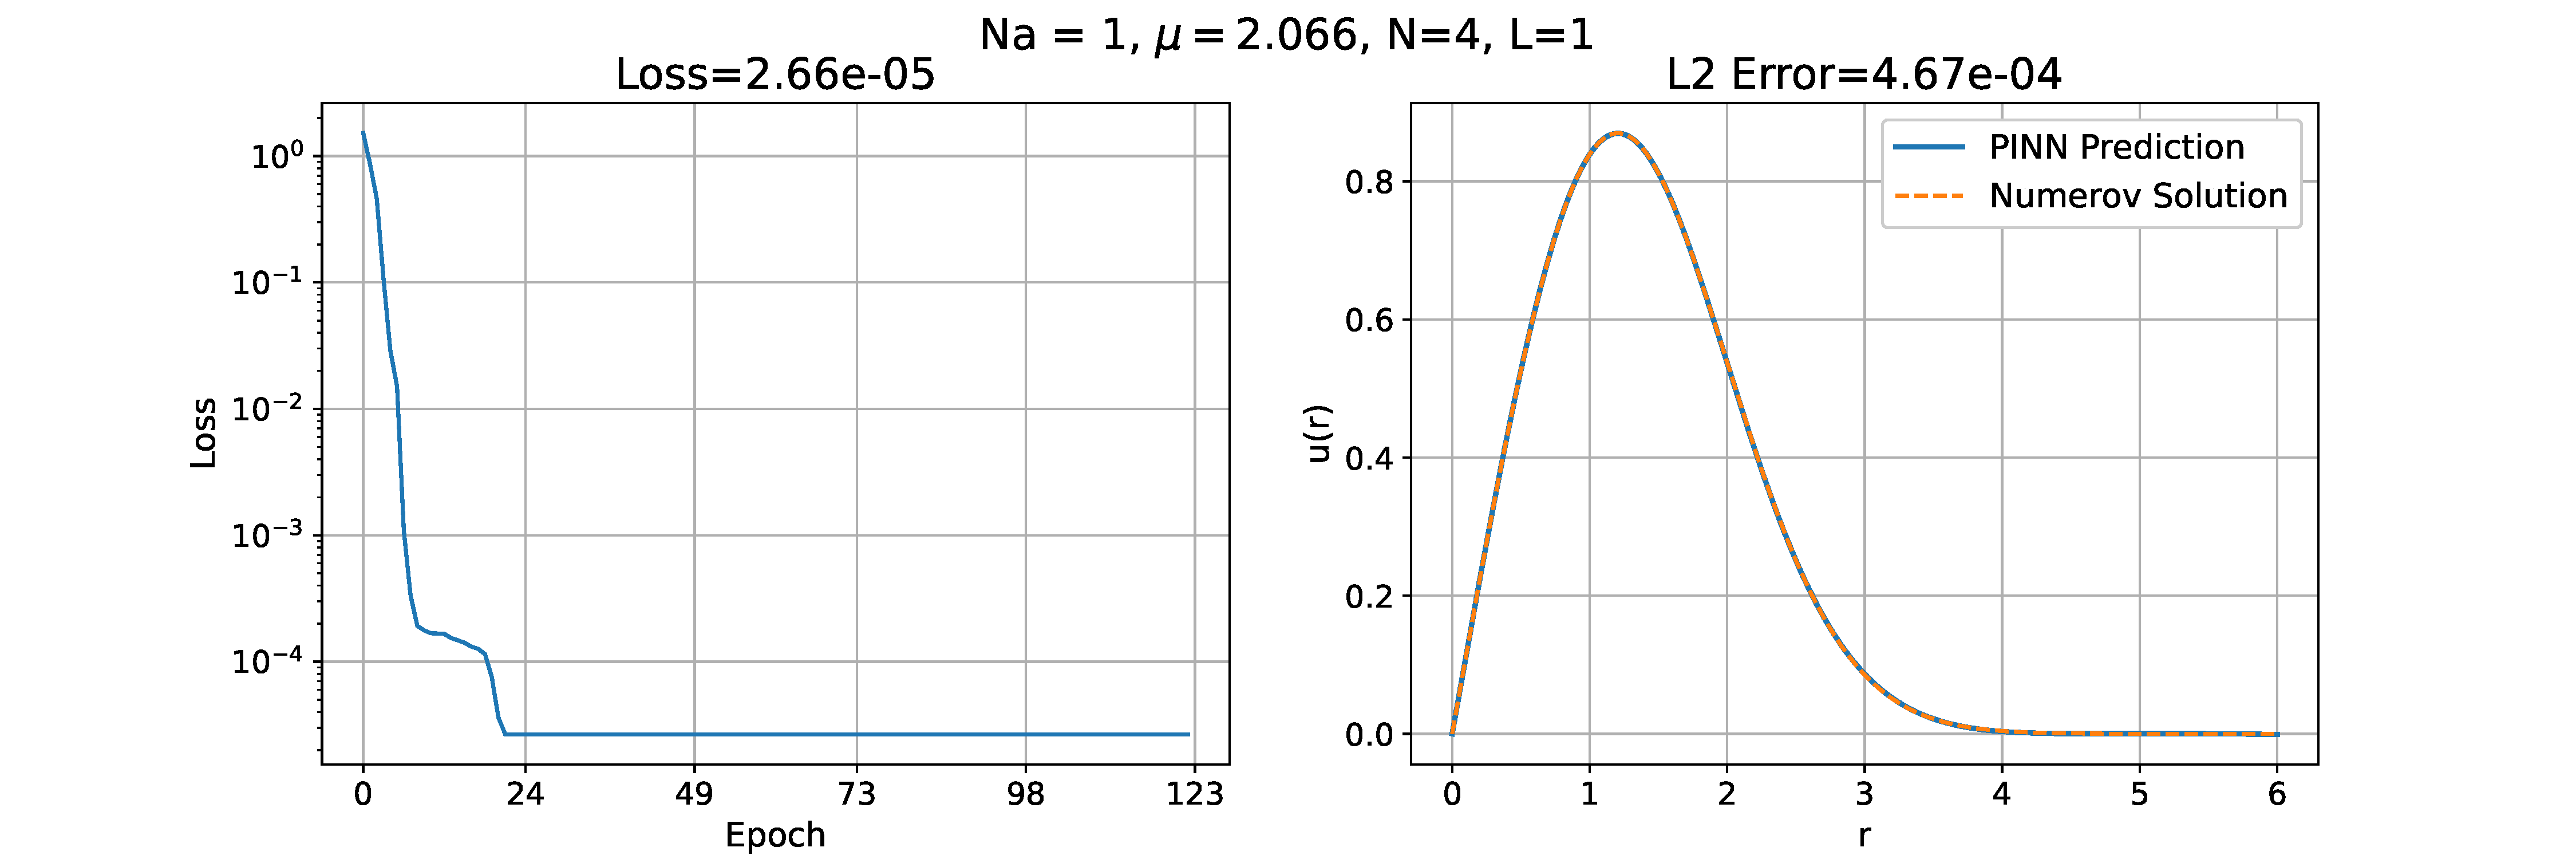
\includegraphics[width=\textwidth]
    {Figures/ex1_N4L1_PINN_Na1.0_x0.00-6.00.png}
    \caption{Results for the 1D GPE with $Na = 1$ using a NN with 1 hidden 
    layer and 4 neurons per layer (N4L1).
    The final loss was $2.66 \times 10^{-5}$, the relative
    $\mathbb L_2$ is $4.67 \times 10^{-4}$ computed with respect to the 
    \texttt{Numerov} solution obtained from the previous reports. 
    \texttt{L-BFGS} optimizer was stopped after 100 iterations with the same
    loss.}
    \label{fig:1d_gpe_N4L1_Na1}
\end{figure}
\begin{figure}[h]
    \centering
    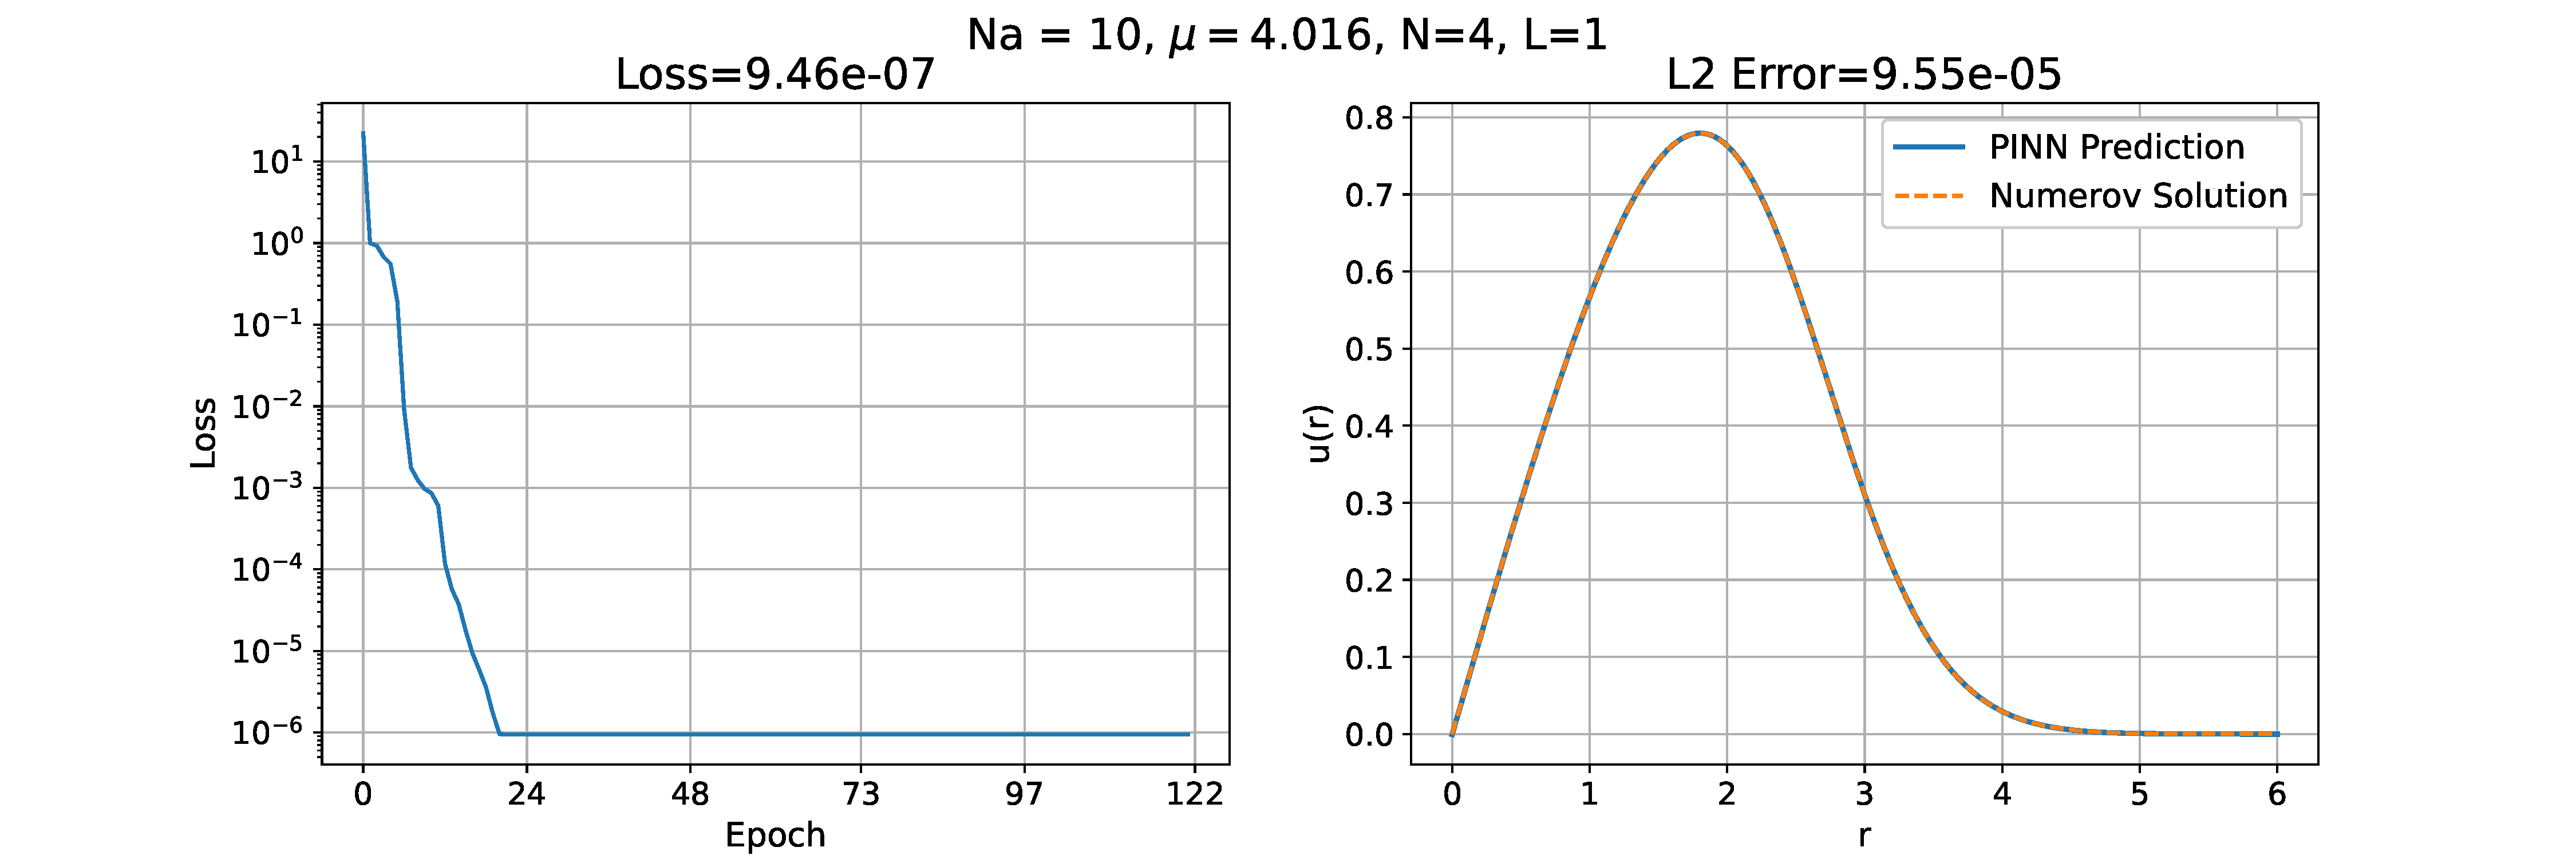
\includegraphics[width=\textwidth]
    {Figures/ex1_N4L1_PINN_Na10.0_x0.00-6.00.png}
    \caption{Results for the 1D GPE with $Na = 10$ using a NN with N4L1.
    The final loss was $9.46 \times 10^{-7}$, the relative
    $\mathbb L_2$ error is $9.55 \times 10^{-5}$ computed with respect to
    the \texttt{Numerov} solution obtained from the previous reports.
    \texttt{L-BFGS} optimizer was stopped after 100 iterations with the same
    loss.}
    \label{fig:1d_gpe_N4L1_Na10}
\end{figure}

More complex architectures with more layers and neurons were tested, but they
didn't show any significant improvement in the results, on the other hand even
smaller NNs gave worse results.
The losses and $\mathbb L_2$ errors for a variety of numbers of neurons and 
layers are reported in Table \ref{tab:1d_gpe} for the $Na = 0$ case, of which 
we know the analytical solution 
\begin{equation*}
    \phi(r) = \frac{2}{\sqrt[4]{\pi}} r e^{-r^2/2}, \quad \mu = \frac{3}{2}.
\end{equation*}

Table \ref{tab:1d_gpe_Npoints} shows instead the effect of changing the number
of sample points used in the training of the NN, always for $Na = 0$, for a
sufficiently complex architecture with N16L3.
After 1000 points the improvement in the $\mathbb L_2$ error is not significant,
but we can positively correlate a low loss with a low $\mathbb L_2$ error, as 
expected.

\begin{table}[htbp]
    \centering
    \begin{tabular}{cccc}
        \toprule
        \textbf{Neurons per Layer} & \textbf{Hidden Layers} & \textbf{Loss}
        & \textbf{$\mathbb{L}_2$ Error} \\
        \midrule
        \multirow{4}{*}{2} 
        & 1 & $7.22 \times 10^{-4}$ & $4.05 \times 10^{-3}$ \\
        & 2 & $7.95 \times 10^{-5}$ & $8.05 \times 10^{-4}$ \\
        & 3 & $3.64 \times 10^{-5}$ & $5.46 \times 10^{-4}$ \\
        & 4 & $6.34 \times 10^{-5}$ & $8.40 \times 10^{-4}$ \\
        \midrule
        \multirow{4}{*}{3} 
        & 1 & $1.65 \times 10^{-4}$ & $1.52 \times 10^{-3}$ \\
        & 2 & $5.77 \times 10^{-6}$ & $1.81 \times 10^{-4}$ \\
        & 3 & $8.90 \times 10^{-6}$ & $2.43 \times 10^{-4}$ \\
        & 4 & $4.19 \times 10^{-6}$ & $6.67 \times 10^{-5}$ \\
        \midrule
        \multirow{4}{*}{4} 
        & 1 & $2.28 \times 10^{-6}$ & $7.95 \times 10^{-5}$ \\
        & 2 & $3.40 \times 10^{-6}$ & $1.18 \times 10^{-4}$ \\
        & 3 & $4.73 \times 10^{-6}$ & $1.71 \times 10^{-4}$ \\
        & 4 & $2.49 \times 10^{-6}$ & $1.30 \times 10^{-4}$ \\
        \midrule
        \multirow{4}{*}{8} 
        & 1 & $5.98 \times 10^{-6}$ & $1.87 \times 10^{-4}$ \\
        & 2 & $2.76 \times 10^{-6}$ & $1.12 \times 10^{-4}$ \\
        & 3 & $3.14 \times 10^{-7}$ & $4.81 \times 10^{-5}$ \\
        & 4 & $3.06 \times 10^{-6}$ & $1.26 \times 10^{-4}$ \\
        \midrule
        \multirow{4}{*}{16} 
        & 1 & $5.84 \times 10^{-6}$ & $1.89 \times 10^{-4}$ \\
        & 2 & $8.90 \times 10^{-7}$ & $6.23 \times 10^{-5}$ \\
        & 3 & $1.78 \times 10^{-6}$ & $1.04 \times 10^{-4}$ \\
        & 4 & $2.69 \times 10^{-6}$ & $8.75 \times 10^{-5}$ \\
        \bottomrule
    \end{tabular}
    \caption{Loss and relative $\mathbb{L}_2$ error for different NN
    architectures for the 1D GPE with $Na = 0$ (analytical solution available).
    Results are consistently good across all architectures from 4 neurons per
    layer, with no clear improvement observed for more complex architectures.}
    \label{tab:1d_gpe}
\end{table}
\begin{table}[h!]
    \centering
    \begin{tabular}{ccc}
        \toprule
        \textbf{Sample Points ($N_f$)} & \textbf{Loss} & \textbf{$\mathbb{L}_2$ Error} \\
        \midrule
        10      & $6.84 \times 10^{-7}$ & $1.97 \times 10^{-2}$ \\
        100     & $1.53 \times 10^{-6}$ & $7.05 \times 10^{-4}$ \\
        500     & $2.40 \times 10^{-6}$ & $1.48 \times 10^{-4}$ \\
        1000    & $8.34 \times 10^{-7}$ & $4.02 \times 10^{-5}$ \\
        5000    & $3.55 \times 10^{-6}$ & $8.42 \times 10^{-5}$ \\
        10000   & $4.05 \times 10^{-6}$ & $1.37 \times 10^{-4}$ \\
        20000   & $9.76 \times 10^{-7}$ & $5.08 \times 10^{-5}$ \\
        \bottomrule
    \end{tabular}
    \caption{Loss and relative $\mathbb{L}_2$ error for different numbers of
    sample points for the 1D GPE with $Na = 0$, using a sufficiently expressive
    NN with N16L3.
    The $\mathbb{L}_2$ error decreases significantly as the number of points 
    increases from 10 to 1000, but does not show a clear improvement beyond that.
    Low loss is generally correlated with low $\mathbb{L}_2$ error, as expected.}
    \label{tab:1d_gpe_Npoints}
\end{table}

Finally, considering the troubles we went through to attempt to solve the GPE
with $Na = 100$ (very strong interaction) with both the \texttt{numerov} and 
the \texttt{variational} method, we were curious to see how the NN would perform 
in this case.
A first run with N4L1 gave only a $3.46 \times 10^{-4}$ loss, but it was
sufficient to increase to N8L2 to get a much better loss of
$1.01 \times 10^{-6}$.
In the previous report the solutions obtained from \texttt{numerov} and the 
\texttt{variational} method were always in good agreement, except for the 
$Na = 100$ case.
It was in fact not clear which of the two methods was giving the correct
solution, as both the procedures showed some flaws in the convergence of the 
parameters, but the PINN training was straightforward, and the result is clearly 
in good agreement with the \texttt{variational} data with a relative 
$\mathbb L_2$ error of $8.99 \times 10^{-5}$
(Figure \ref{fig:1d_gpe_N8L2_Na100}).

\begin{figure}[h]
    \centering
    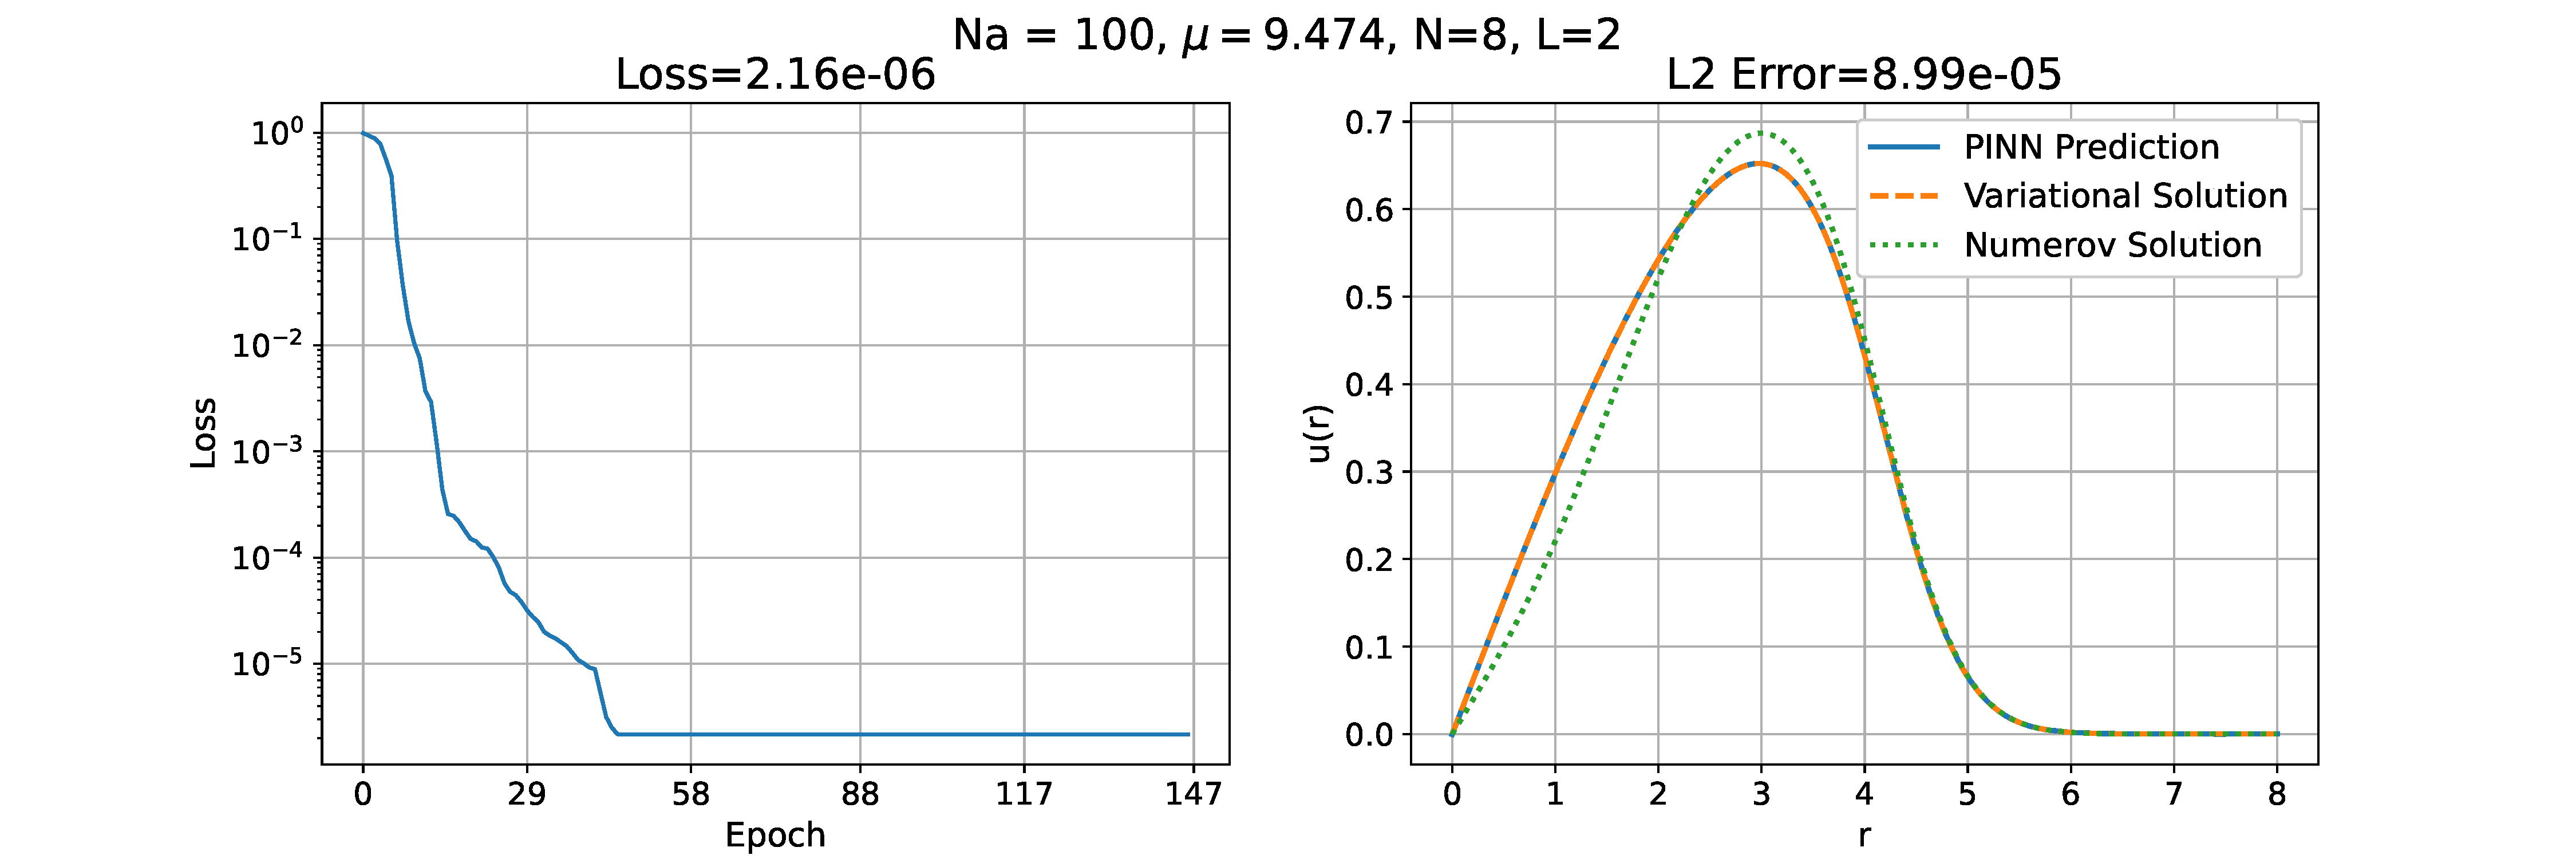
\includegraphics[width=\textwidth]{Figures/ex1_N8L2_PINN_Na100.0_x0.00-8.00.png}
    \caption{Results for the 1D GPE with $Na = 100$ using a NN with N8L2.
    The relative $\mathbb L_2$ is $8.99 \times 10^{-5}$ computed with respect to 
    the data obtained from the previous reports with the \texttt{variational} 
    method.
    \texttt{L-BFGS} optimizer was stopped after 100 iterations with the same
    loss.}
    \label{fig:1d_gpe_N8L2_Na100}
\end{figure}




\section{Time-dependent \gpe} \label{sec:gpe_time}

We can now move to a 2D problem by replicating the example 3.1.1 in
\cite{RAISSI2019686}, where the authors solve a nonlinear Schr\"{o}dinger 
equation with boundary conditions
\begin{align*}
    &ih_t + 0.5h_{xx} + |h|^2 h = 0,
    \quad x \in [-5, 5], \quad t \in [0, \pi/2], \\
    &h(0, x) = 2\,\sech (x), \\
    &h(t, -5) = h(t, 5), \\
    &h_x(t, -5) = h_x(t, 5),
\end{align*}
where the subscripts denote partial derivatives. This corresponds to the
evolution of a soliton solution with unitary interaction and no potential
under the time-dependent GPE.

In this case the solution is complex, so we need to separate real and imaginary
parts $h(t, x) = u(t, x) + iv(t, x)$, such that
\begin{equation}
    \mathcal N(t, x) = [u(t, x), ~ v(t, x)]
\end{equation}
where $\mathcal N$ is a multi-output NN with 2 inputs and 2 outputs.

The loss function is defined as
\begin{align*}
    \mathcal L &= \mathcal L_{\rm PDE} + \mathcal L_{\rm IC} + \mathcal L_{\rm BC} \\
    \mathcal L_{\rm PDE} &= \frac{1}{N_f} \sum_{i=1}^{N_f}
    \left| ih_t(t_i, x_i) + 0.5h_{xx}(t_i, x_i) + |h(t_i, x_i)|^2 h(t_i, x_i) \right|^2 \\
    \mathcal L_{\rm IC} &= \frac{1}{N_0} \sum_{i=1}^{N_0}
    |h(0, x_i) - 2\,\sech (x_i)|^2 \\
    \mathcal L_{\rm BC} &= \frac{1}{N_b} \sum_{i=1}^{N_b}
    |h(t_i, -5) - h(t_i, 5)|^2 + |h_x(t_i, -5) - h_x(t_i, 5)|^2
\end{align*}
where we now have $N_0$ points for the initial condition and $N_b$ points to
enforce the symmetry of the solution at the boundaries.
Given that we have a non-zero initial condition there is no need to enforce the
normalization this time.
We use $N_f = 20000$, $N_0 = 50$ and $N_b = 50$ points, all distributed with LHS
in the appropriate intervals, as it was done by
\cite{RAISSI2019686}.

The increased dimensionality of the problem forces us to use a more complex NN
architecture as the first attempts with only 4--8 neurons and 1--2 hidden layers
could not go below a loss of $10^{-2}$.
Eventually a first satisfactory result was obtained with N16L3, with a loss of
$1.28 \times 10^{-4}$.
Figure \ref{fig:2d_gpe_N32L3} shows the results for an even bigger NN with
N32L3, with a loss of $1.86 \times 10^{-5}$.

\begin{figure}[h]
    \centering
    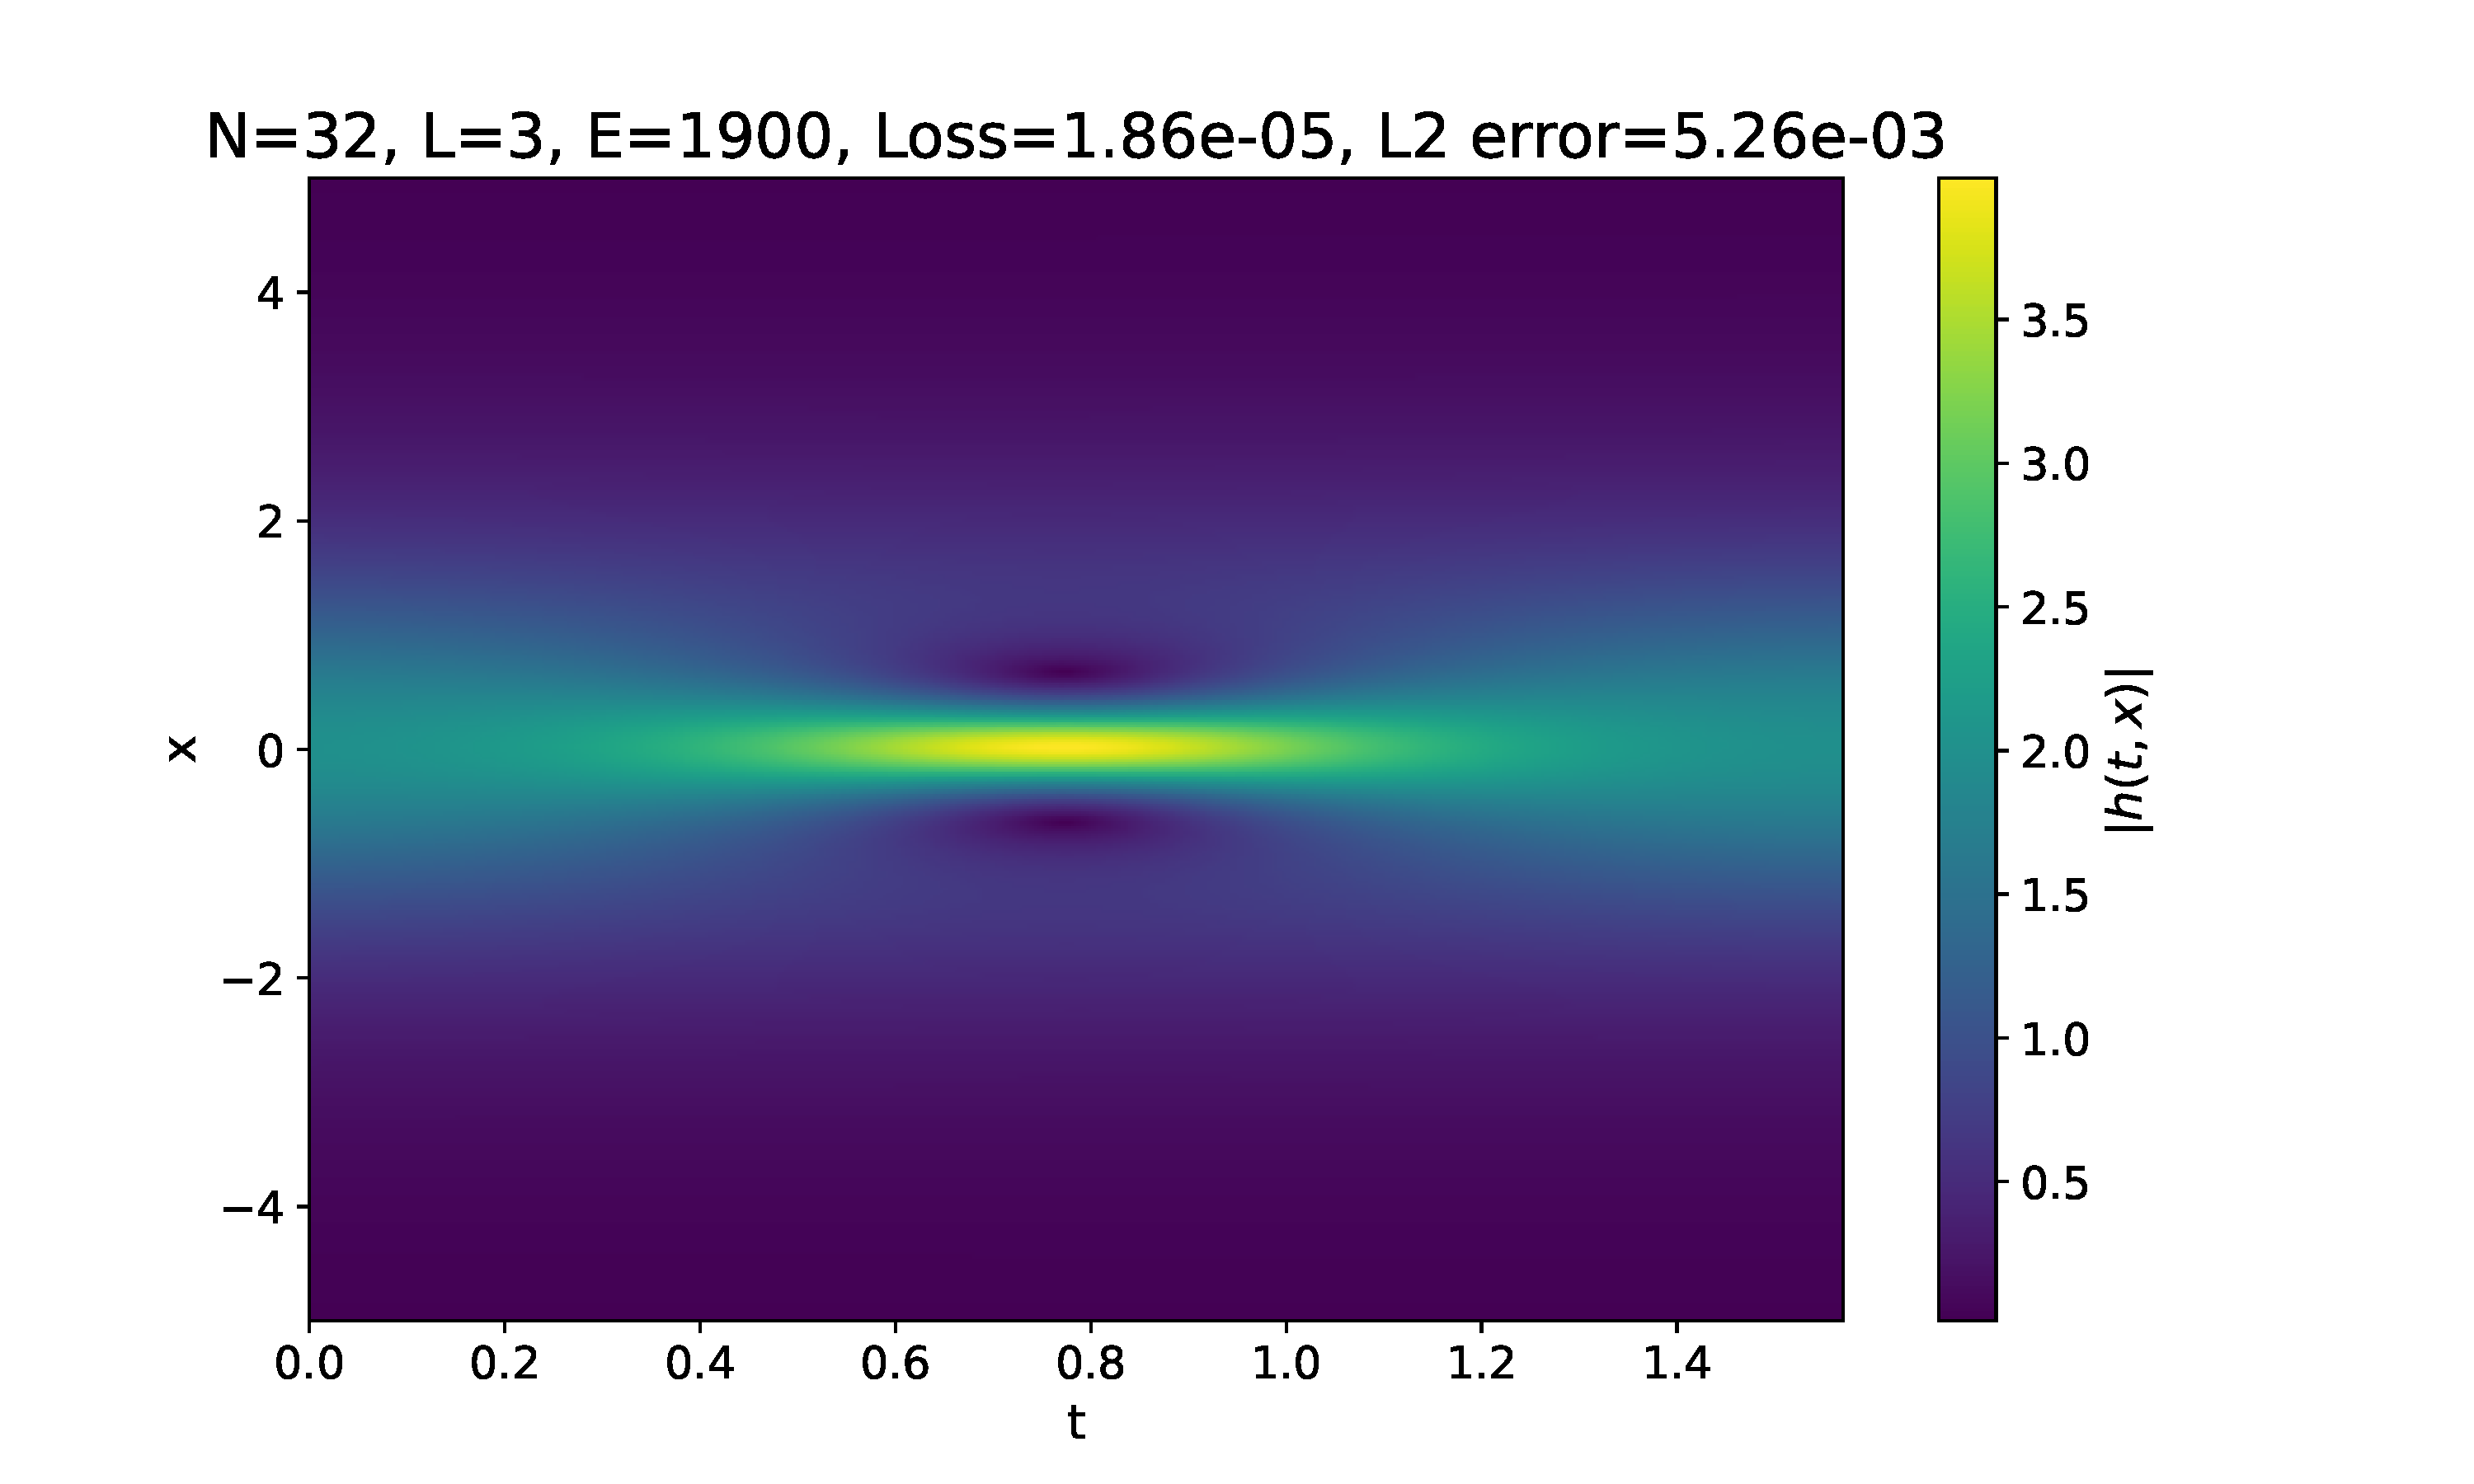
\includegraphics[width=\textwidth]{Figures/ex2_N32L3_PINN_E1900_t0.00-1.57_x-5.00-5.00_lbfgs_heatmap.png}
    \caption{Results for the time-dependent GPE with a NN with N32L3.
    The relative $\mathbb L_2$ is $5.26 \times 10^{-3}$ computed with respect to
    the analytical solution. \texttt{L-BFGS} optimizer was stopped after 100
    iterations with the same loss.}
    \label{fig:2d_gpe_N32L3}
\end{figure}

Thanks to the data of the exact solution provided in the GitHub repository of
\cite{RAISSI2019686} (\url{https://github.com/maziarraissi/PINNs})
we can also compute the relative $\mathbb L_2$ error of our solution with 
respect to the analytical one, which gave $1.45 \times 10^{-2}$ for the first
satisfactory result and $5.26 \times 10^{-3}$ for the bigger NN, showing again
that a lower loss correlates with a better solution.
Considering that Raissi et al. used a N100L5 NN and obtained a relative
$\mathbb L_2$ error of $1.97 \times 10^{-3}$, we are very satisfied with our
results.

Figure \ref{fig:2d_gpe_N32L3_slice} shows some slices of the solution for the 
bigger NN to appreciate the agreement with the analytical solution, even in the
highly nonlinear regions of the domain.

\begin{figure}[h!]
    \centering
    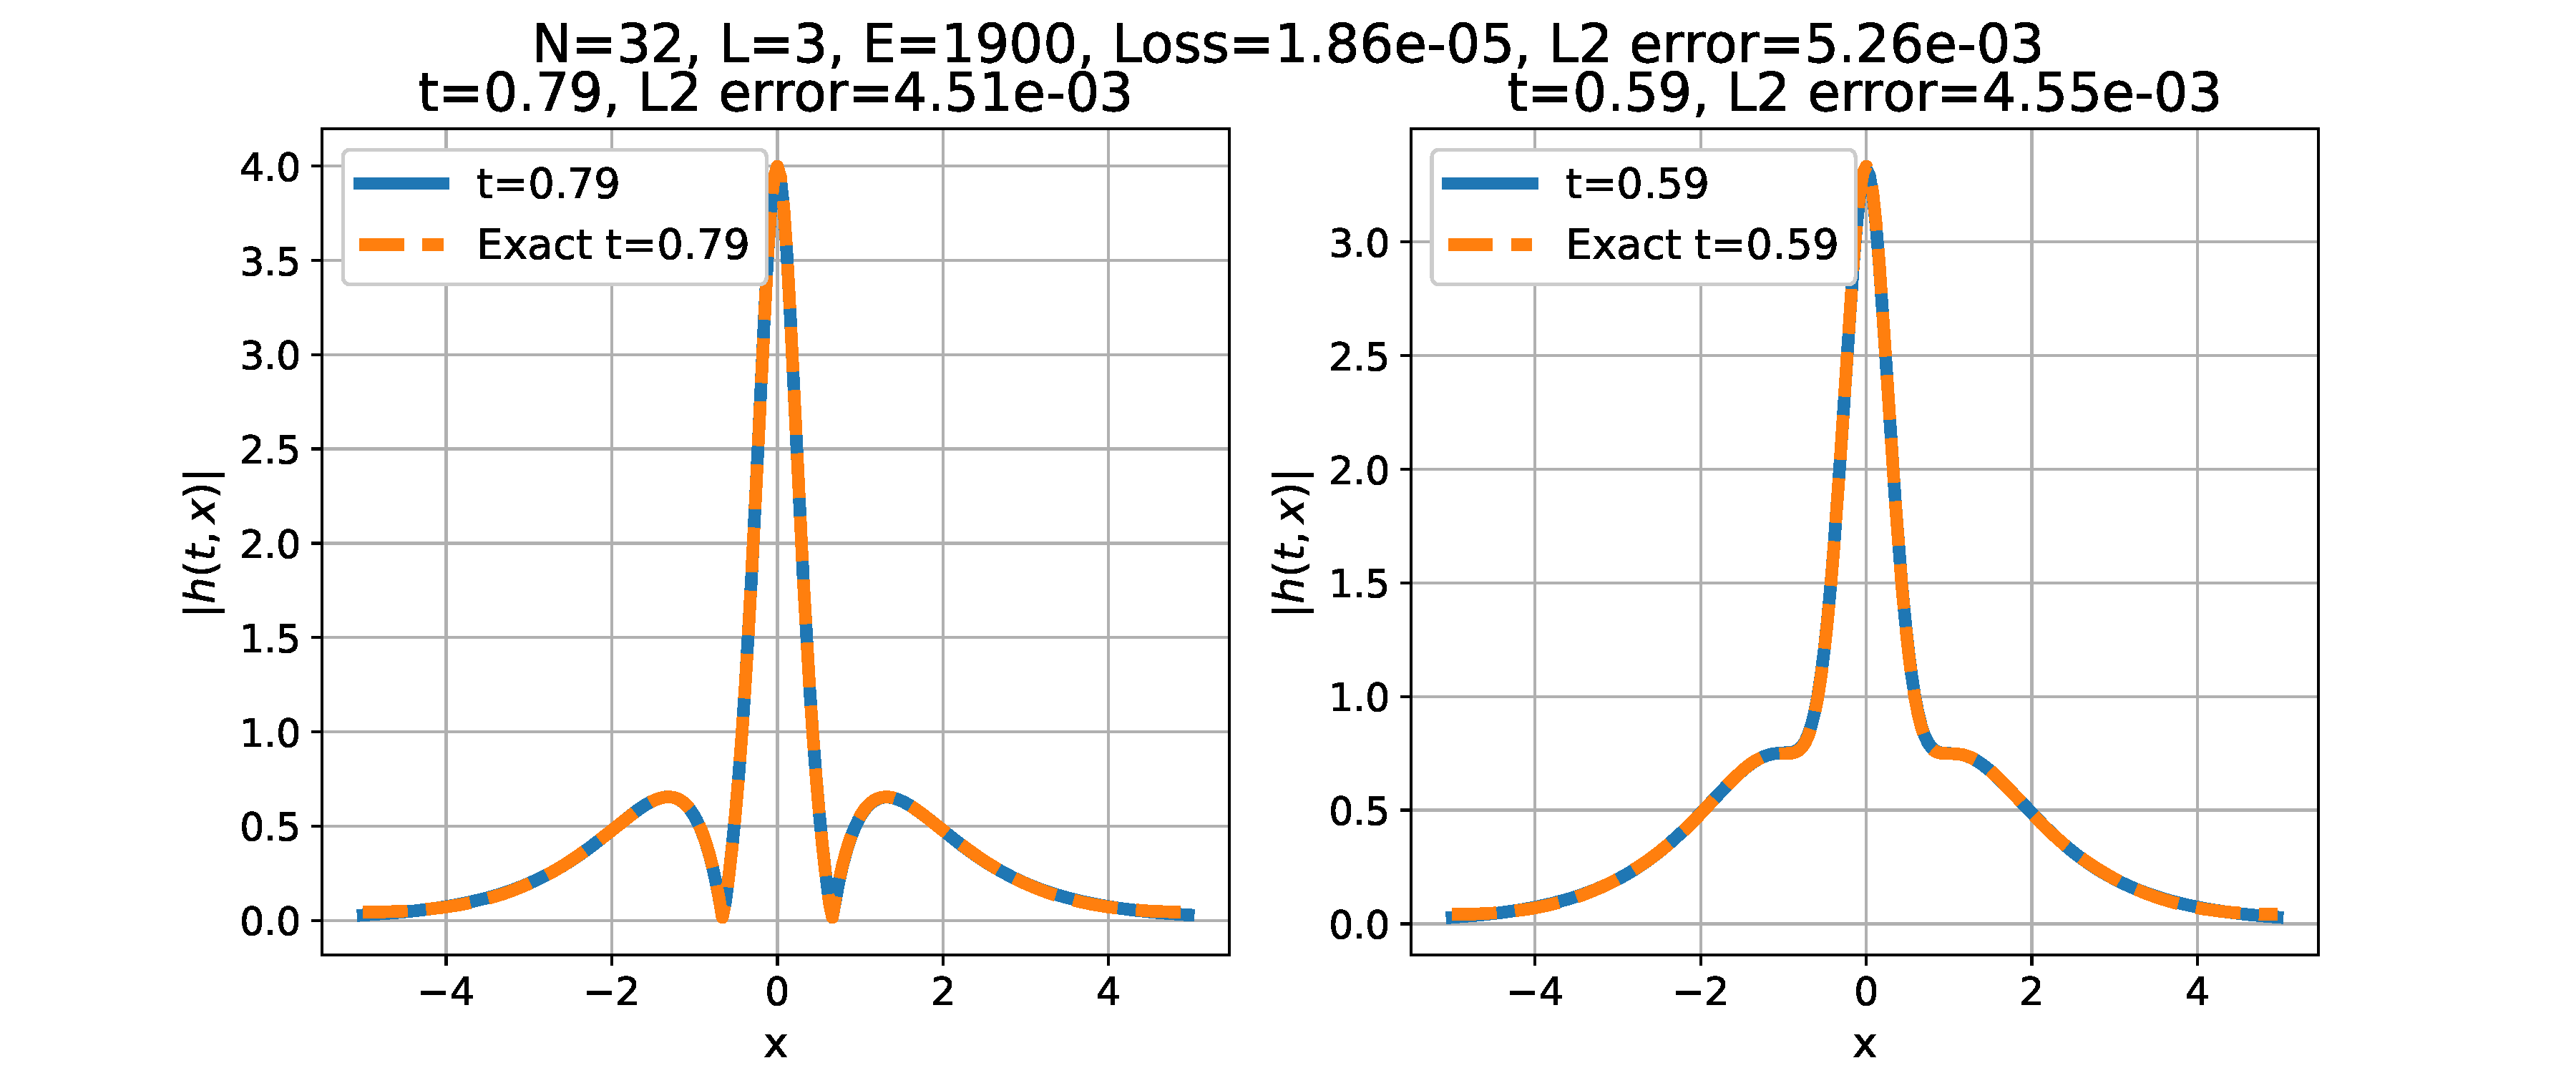
\includegraphics[width=\textwidth]{Figures/ex2_N32L3_PINN_E1900_t0.00-1.57_x-5.00-5.00_lbfgs_slice.png}
    \caption{Slices of the results for the time-dependent GPE with N32L3.
    We can appreciate the NN ability to capture the solution even in the highly 
    nonlinear regions of the domain.}
    \label{fig:2d_gpe_N32L3_slice}
\end{figure}




\section{Ground States of the GPE in Various Trapping Potentials} \label{sec:double_well}

To further test the reliability of the method we now explore the capability of
the NN to solve the GPE with a double well potential.

\subsection{1D Double Well} \label{sec:1d_double_well}

We report here the GPE in 1D
\begin{equation*}
    -\frac{1}{2} \dv[2]{\psi(x)}{x} 
    + \left(V_{\rm ext}(x) + g |\psi(x)|^2 - \mu\right) \psi(x) = 0
\end{equation*}
where $V_{\rm ext}(x)$ is a potential of our choice, $g$ is the interaction
strength and $\mu$ is the chemical potential, which is again a trainable 
parameter.

We will solve the problem in $x \in [x_l, x_r]$ depending on the potential and
asking for $\psi(x_l) = \psi(x_r) = 0$ as boundary conditions, which are
physically reasonable.

Starting from a symmetric double well potential
\begin{equation}
    V_{\rm ext}(x) = \left(x^2 - a\right)^2
    \label{eq:dw}
\end{equation}
with $a = 1, 2$ so that the middle barrier is respectively $V(0) = 1$ and
$V(0) = 4$.
We can use $\mathcal L_{\rm PDE}$ with 1000 sample points, $\mathcal L_{\rm BC}$
and $\mathcal L_{\rm norm}$ losses like the ones in \eqref{eq:ex1_loss}.
The results are shown in Figures \ref{fig:ex3_dw1_easy} and
\ref{fig:ex3_dw2_oops} for a NN with N4L2 and $g = 1$.

\begin{figure}[h]
\begin{minipage}{0.48\textwidth}
    \centering
    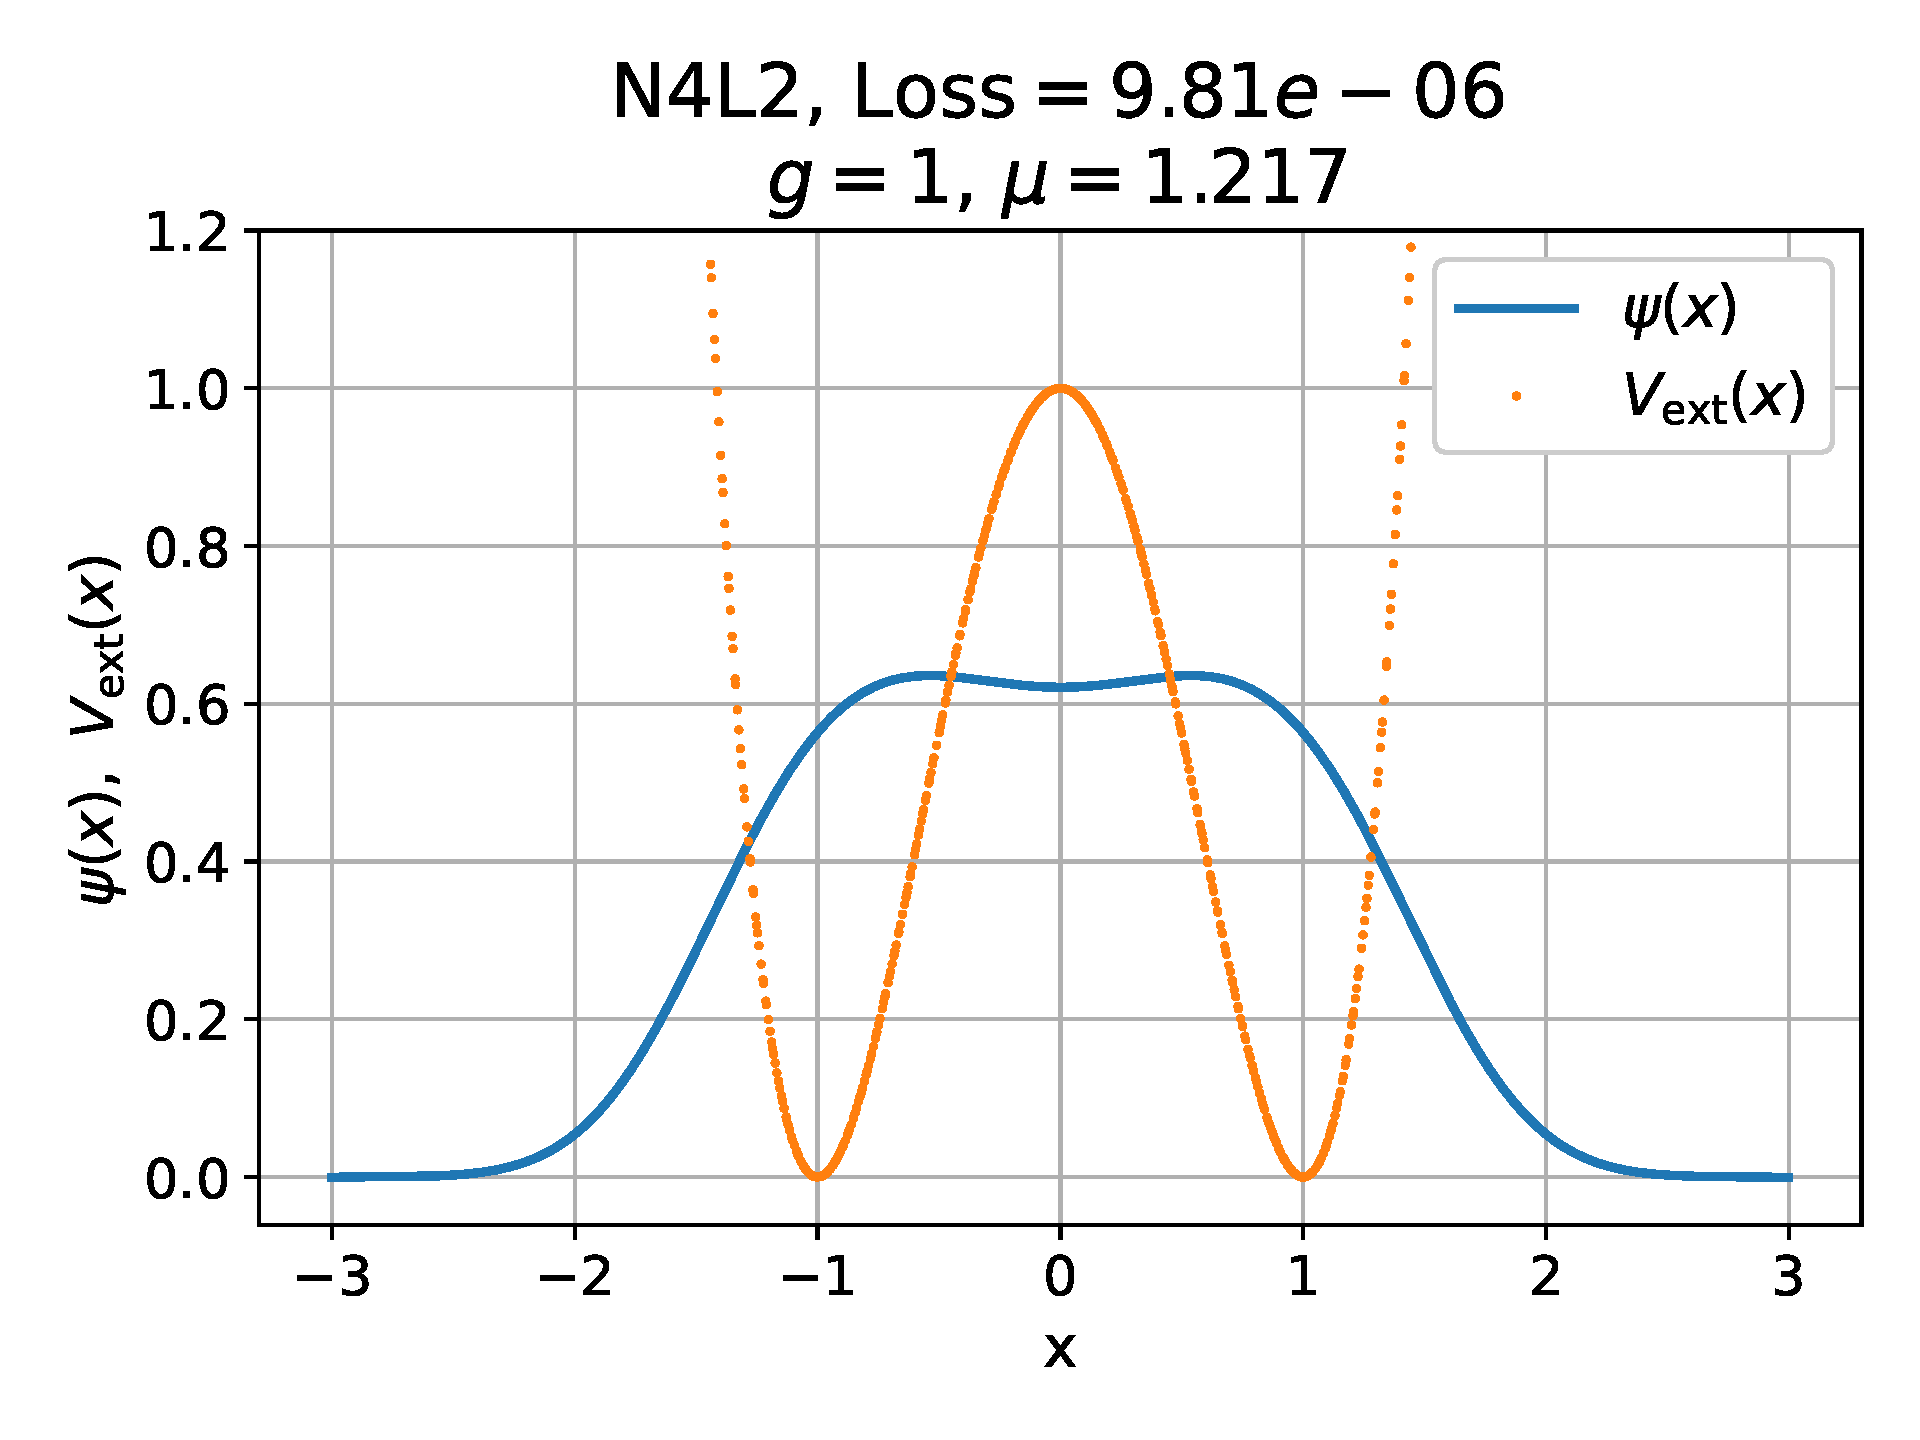
\includegraphics[width=\textwidth]{Figures/ex3_1D_N4L2_g1_dw1.png}
    \caption{Results for the 1D GPE with the symmetric double well potential 
    from equation \eqref{eq:dw} with $a = 1$ and $g = 1$ using a NN with N4L2.}
    \label{fig:ex3_dw1_easy}
\end{minipage}
\hspace{0.05\textwidth}
\begin{minipage}{0.48\textwidth}
    \centering
    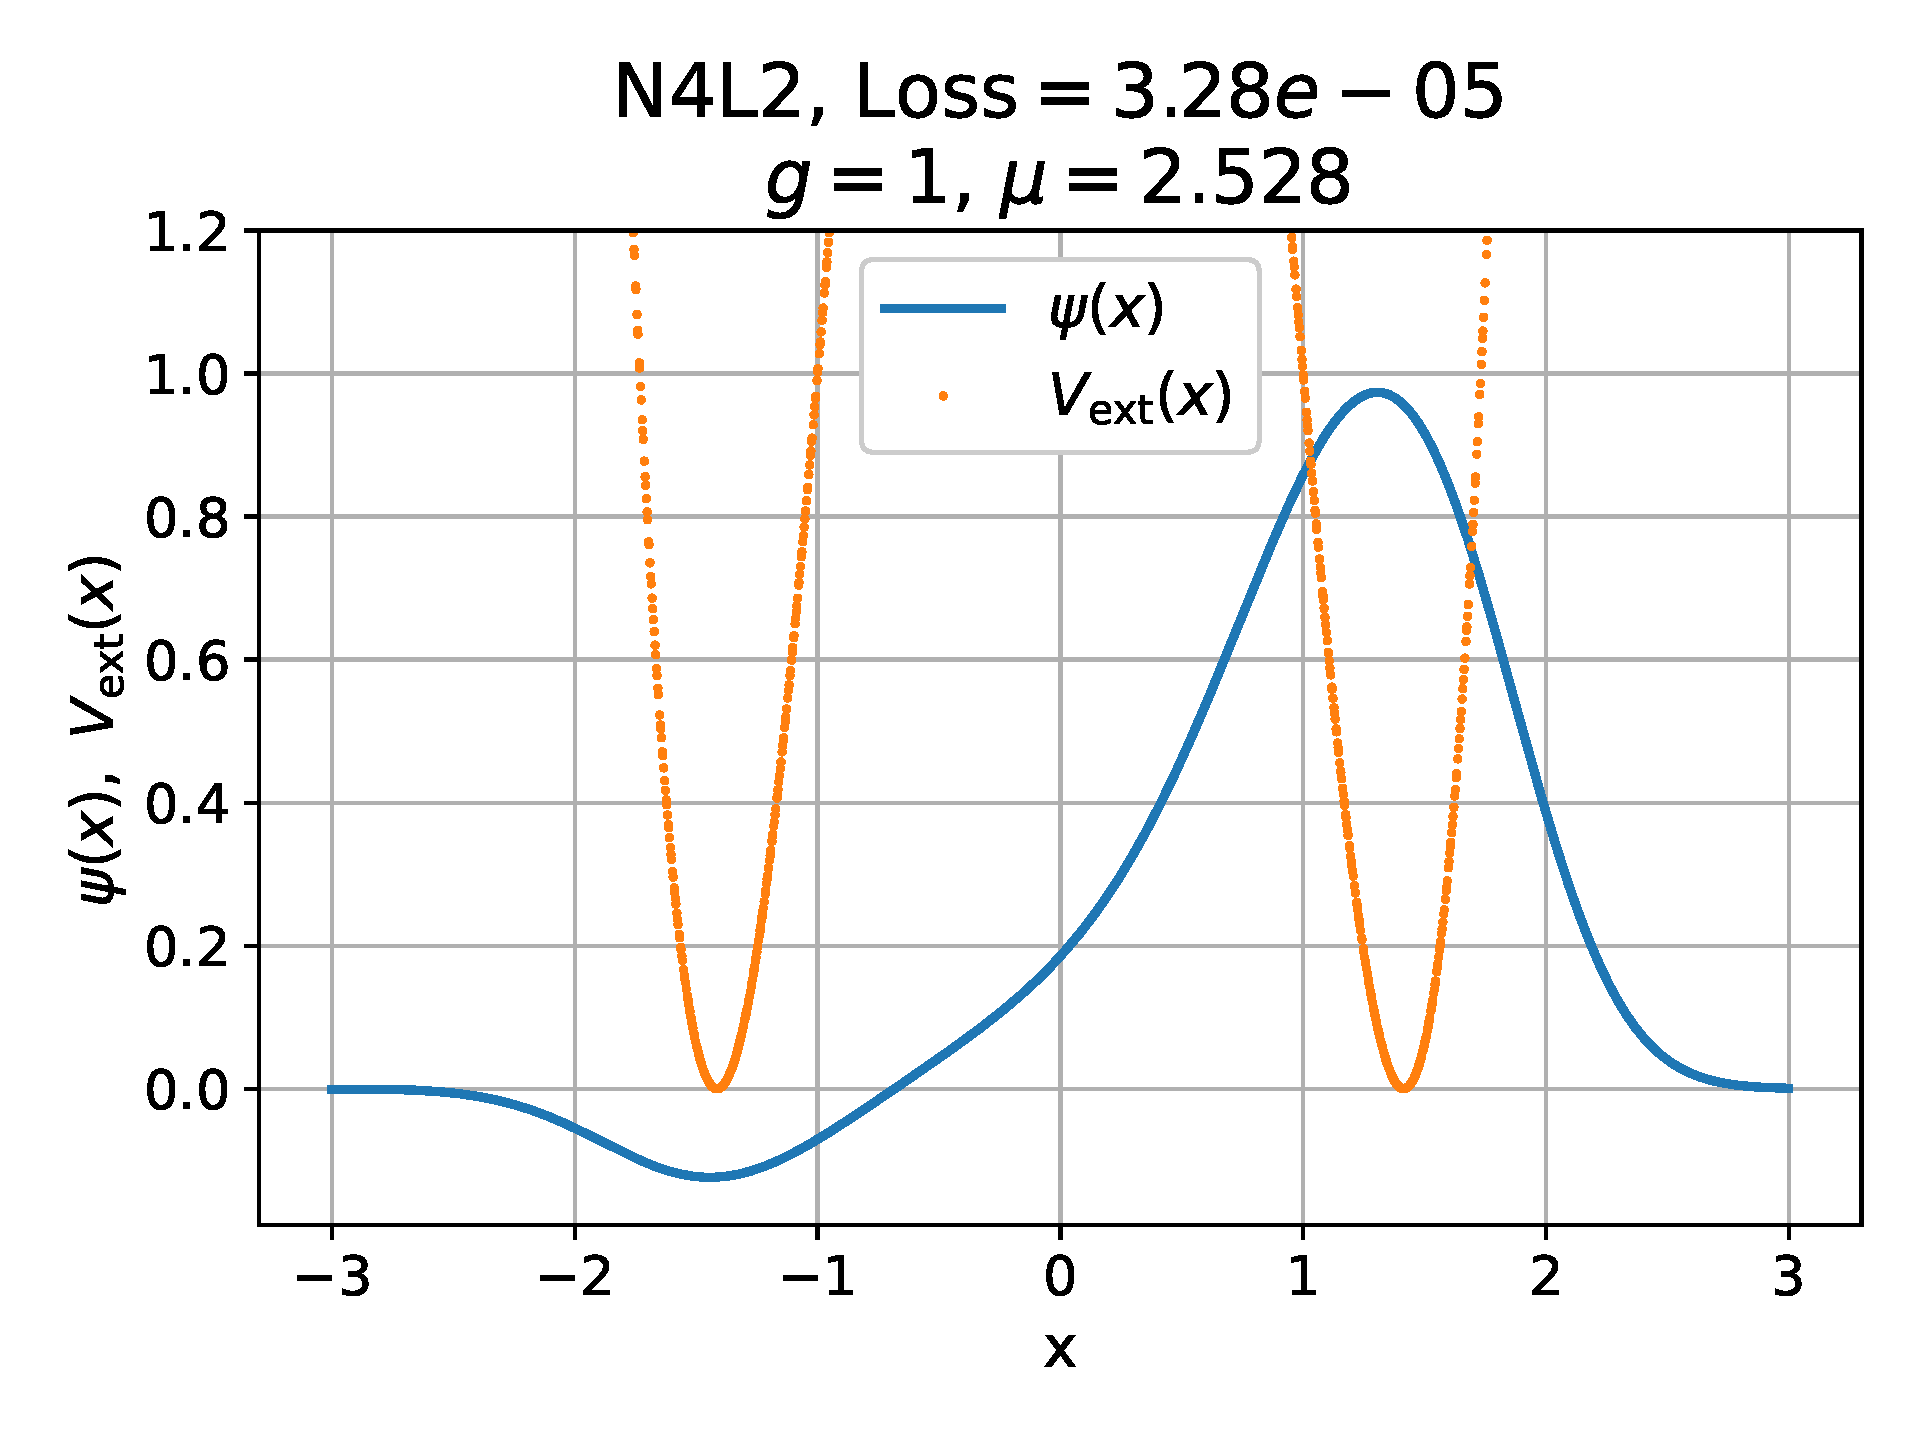
\includegraphics[width=\textwidth]{Figures/ex3_1D_N4L2_g1_dw2.png}
    \caption{Results for the 1D GPE with the symmetric double well potential
    from equation \eqref{eq:dw} with $a = 2$ and $g = 1$ using a NN with N4L2.}
    \label{fig:ex3_dw2_oops}
\end{minipage}
\end{figure}

We notice immediately that for the case $a = 1$ we found the ground state
solution, while for $a = 2$ our wave function has a node, is not symmetric and
has a higher $\mu$.
This is a clear sign that we found an excited state solution, or not even a
physical one.

To help the optimizer find the ground state, we can incorporate a physical
constraint that we have so far neglected: the positivity of the wave function.
We enforce this by appending a \texttt{pytorch.nn.Softplus()} layer at the end
of the neural network, which ensures a smooth, strictly positive output.
\footnote{In practice, enforcing positivity caused the optimizer to become
stuck at a loss value of 1, corresponding $\psi(x) \equiv 0$.
To overcome this issue, we strengthened the normalization constraint by
increasing its weight,
$\mathcal{L}_{\rm norm} \rightarrow 5\,\mathcal{L}_{\rm norm}$,
which encouraged the network to grow away from the trivial solution.}
Unfortunately this method alone did not succeed as the NN was still trying to 
approximate the excited state and the optimizer got stuck in a high loss local 
minimum.
We also tried to initialize the weights of the NN with a gaussian, but the
result is always the same (even increasing the NN complexity or the sample
points) and is shown in Figure \ref{fig:ex3_dw2_shit}.

\begin{figure}[h]
\begin{minipage}{0.48\textwidth}
    \centering
    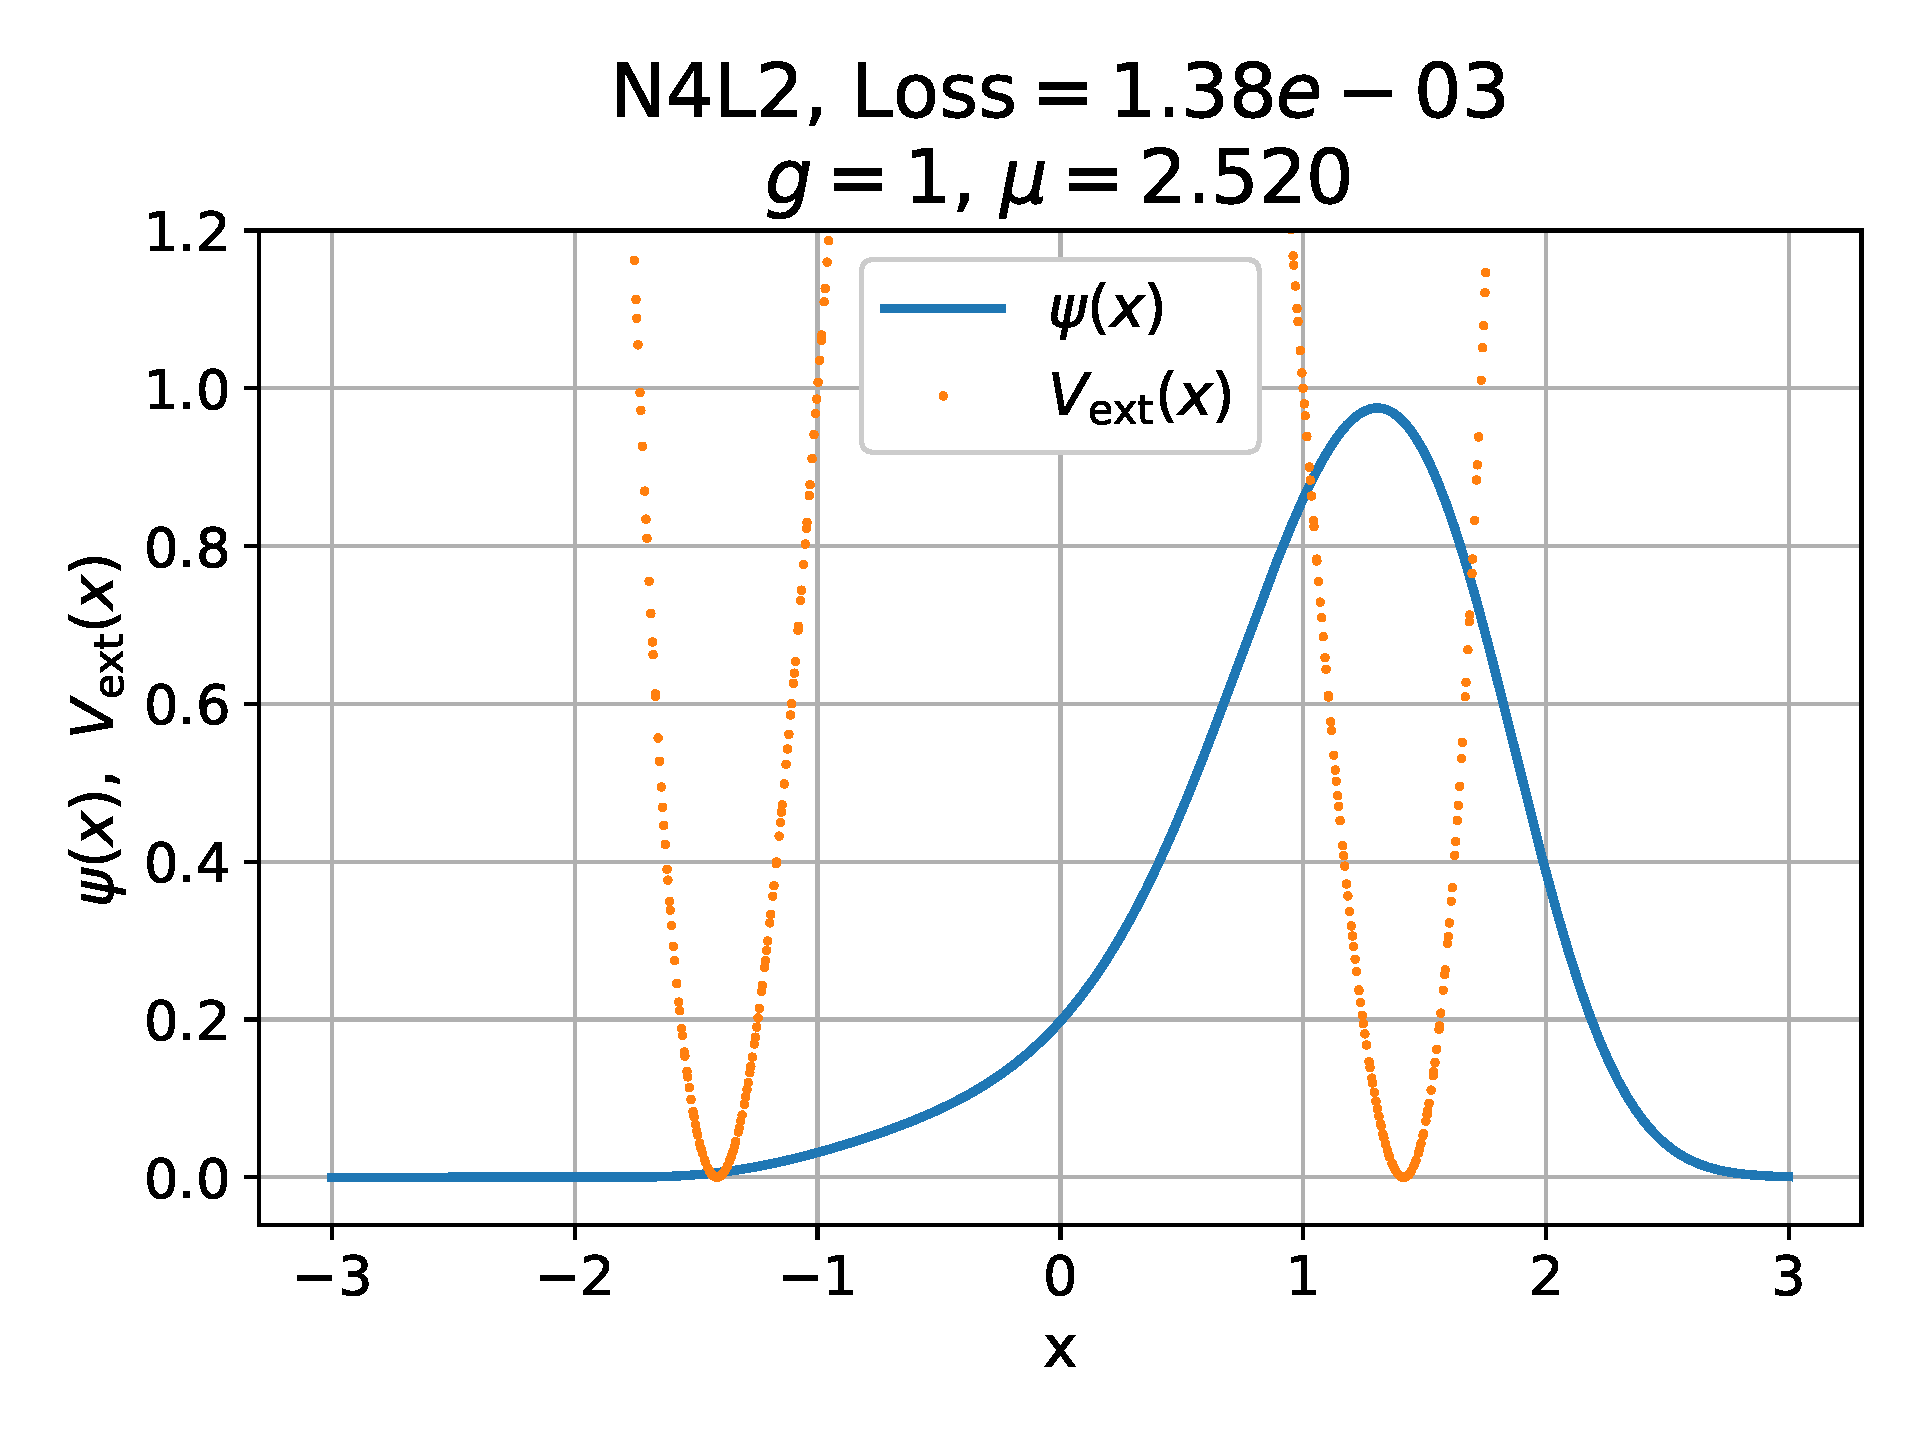
\includegraphics[width=\textwidth]{Figures/ex3_1D_N4L2_pos_g1_dw2_gauss.png}
    \caption{Another failed attempt at finding the ground state of the system
    under the potential in equation \eqref{eq:dw}, this time we also tried to
    enforce positivity and used a gaussian initialization. 
    Increasing the NN complexity or the number of sample points had no effect.}
    \label{fig:ex3_dw2_shit}
\end{minipage}
\hspace{0.05\textwidth}
\begin{minipage}{0.48\textwidth}
    \centering
    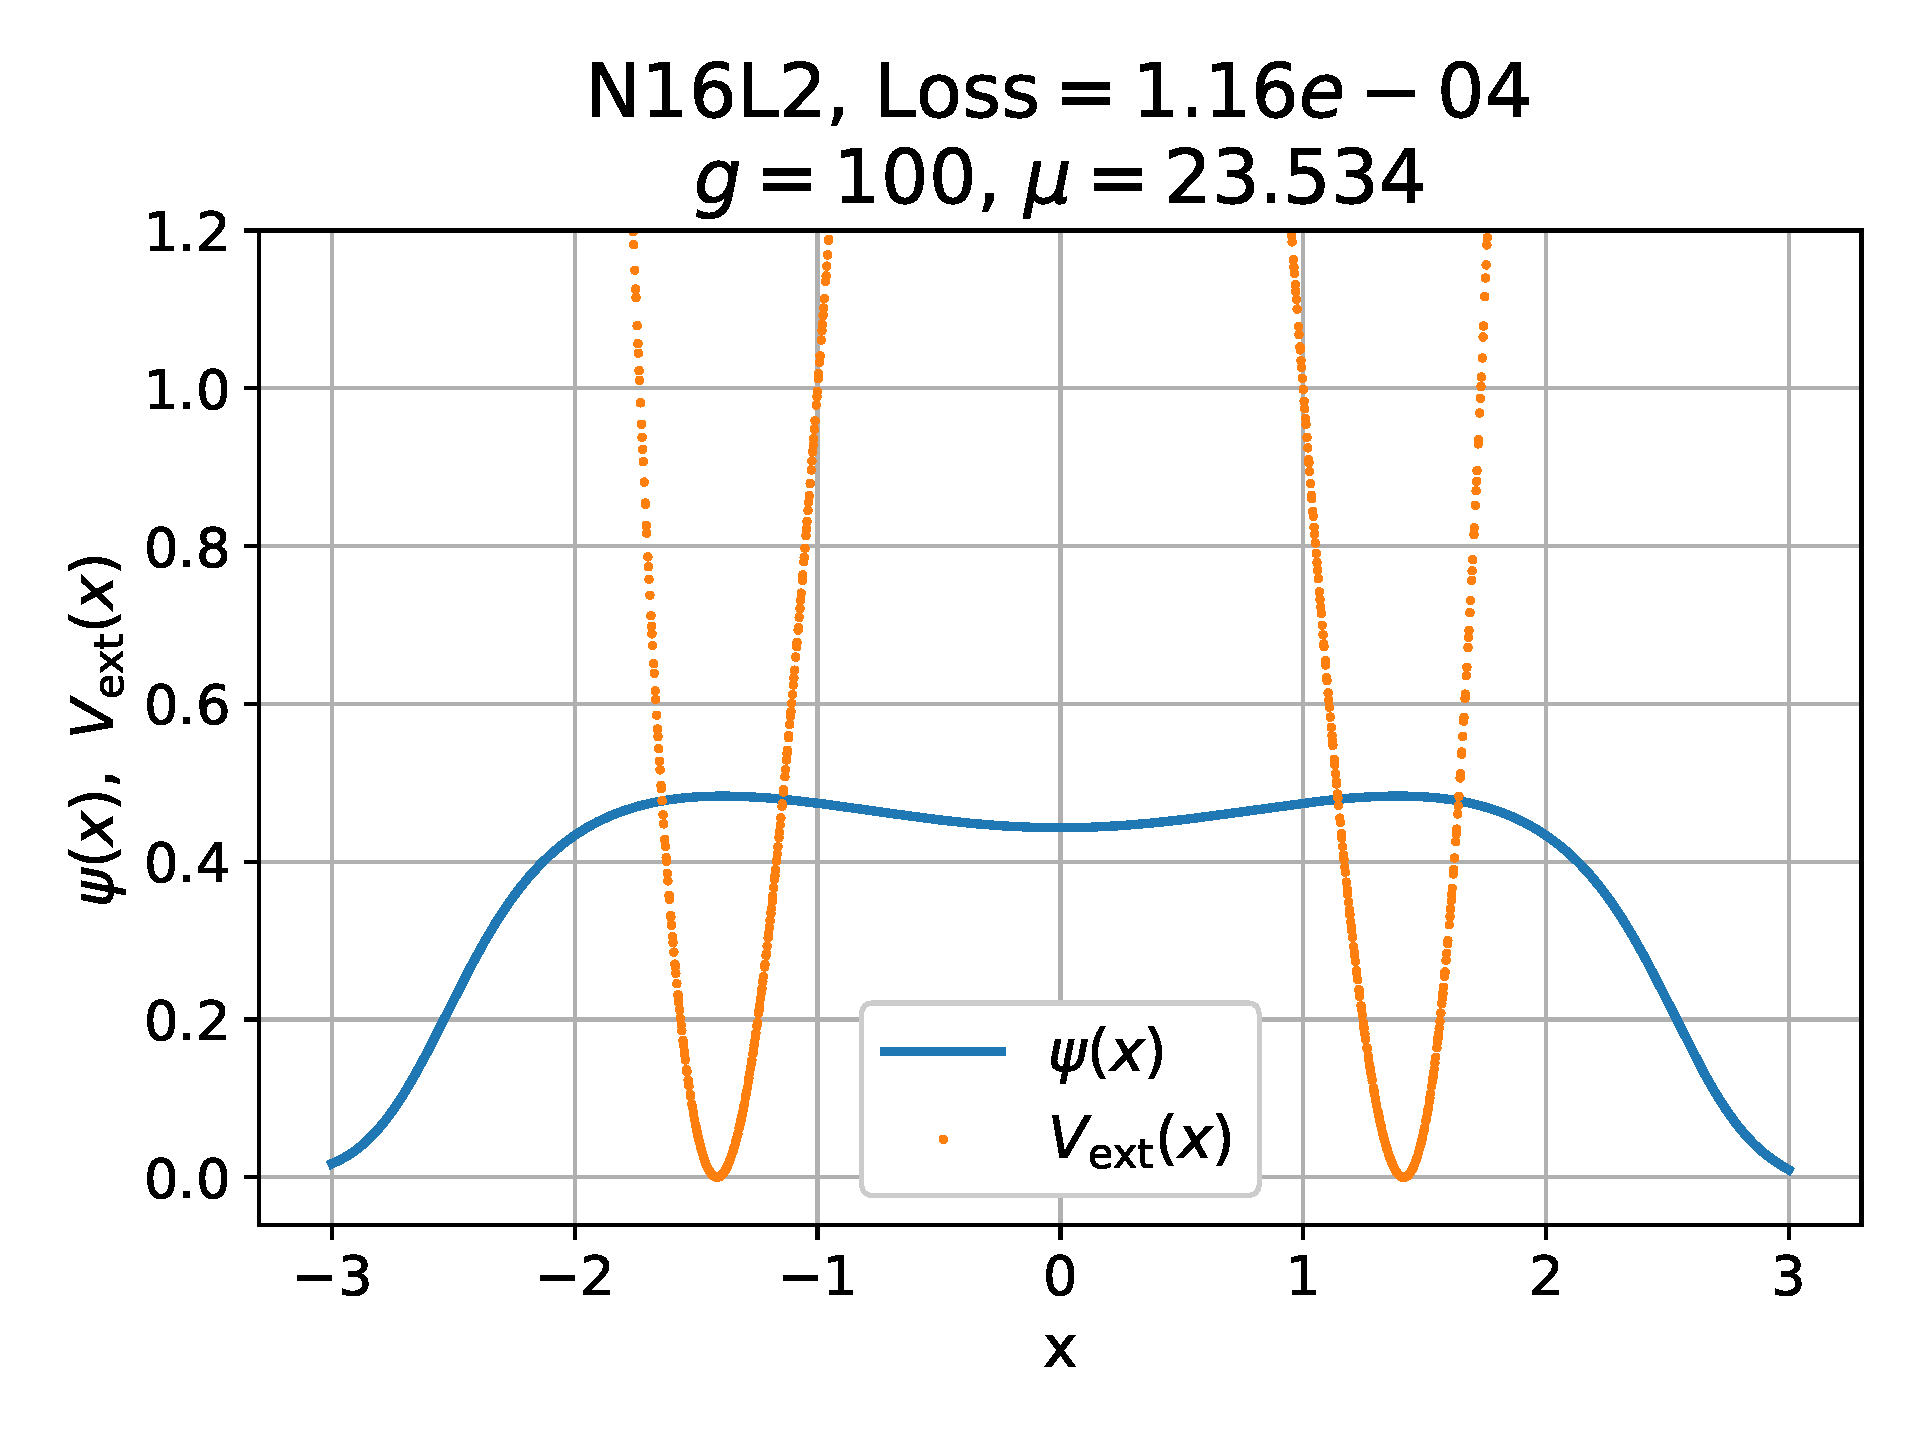
\includegraphics[width=\textwidth]{Figures/ex3_1D_N16L2_pos_g100_dw2_gauss.png}
    \caption{Increasing the strength of the interaction forces the wave function
    to expand over both the wells. 
    This time we are confident that we found the ground state given the symmetry
    and the Loss of $2.9 \times 10^{-4}$. \\}
    \label{fig:ex3_dw2_yee_g100}
\end{minipage}
\end{figure}

What ultimately worked was increasing g to 100, so that the system was highly
interacting, allowing the wave function to freely spread over the domain.
In this case we found that a N16L2 NN helped, and the results are shown in Figure
\ref{fig:ex3_dw2_yee_g100}.
\footnote{The reader might wonder whether relaxing the normalization to 
$\int|\psi|^2\,dx = \alpha, ~ \alpha > 1$ would have worked too.
Indeed, under the rescaling $\psi \mapsto \sqrt{\alpha}\,\psi$ one has
$|\psi|^2 \mapsto \alpha|\psi|^2$, which is equivalent to $g \mapsto \alpha g$.
Thus, the two approaches are physically identical, and increasing $g$ 
was simply the more natural knob to turn, that also kept $\psi$ normalized to 1.}
Now we can start from the NN trained at $g = 100$, and optimize it for $g=1$,
the result is shown in Figure \ref{fig:ex3_dw2_yee_g1}.
In this case we also find beneficial to increase the number of sample points to
2000.

\begin{figure}[h!]
\begin{minipage}{0.48\textwidth}
    \centering
    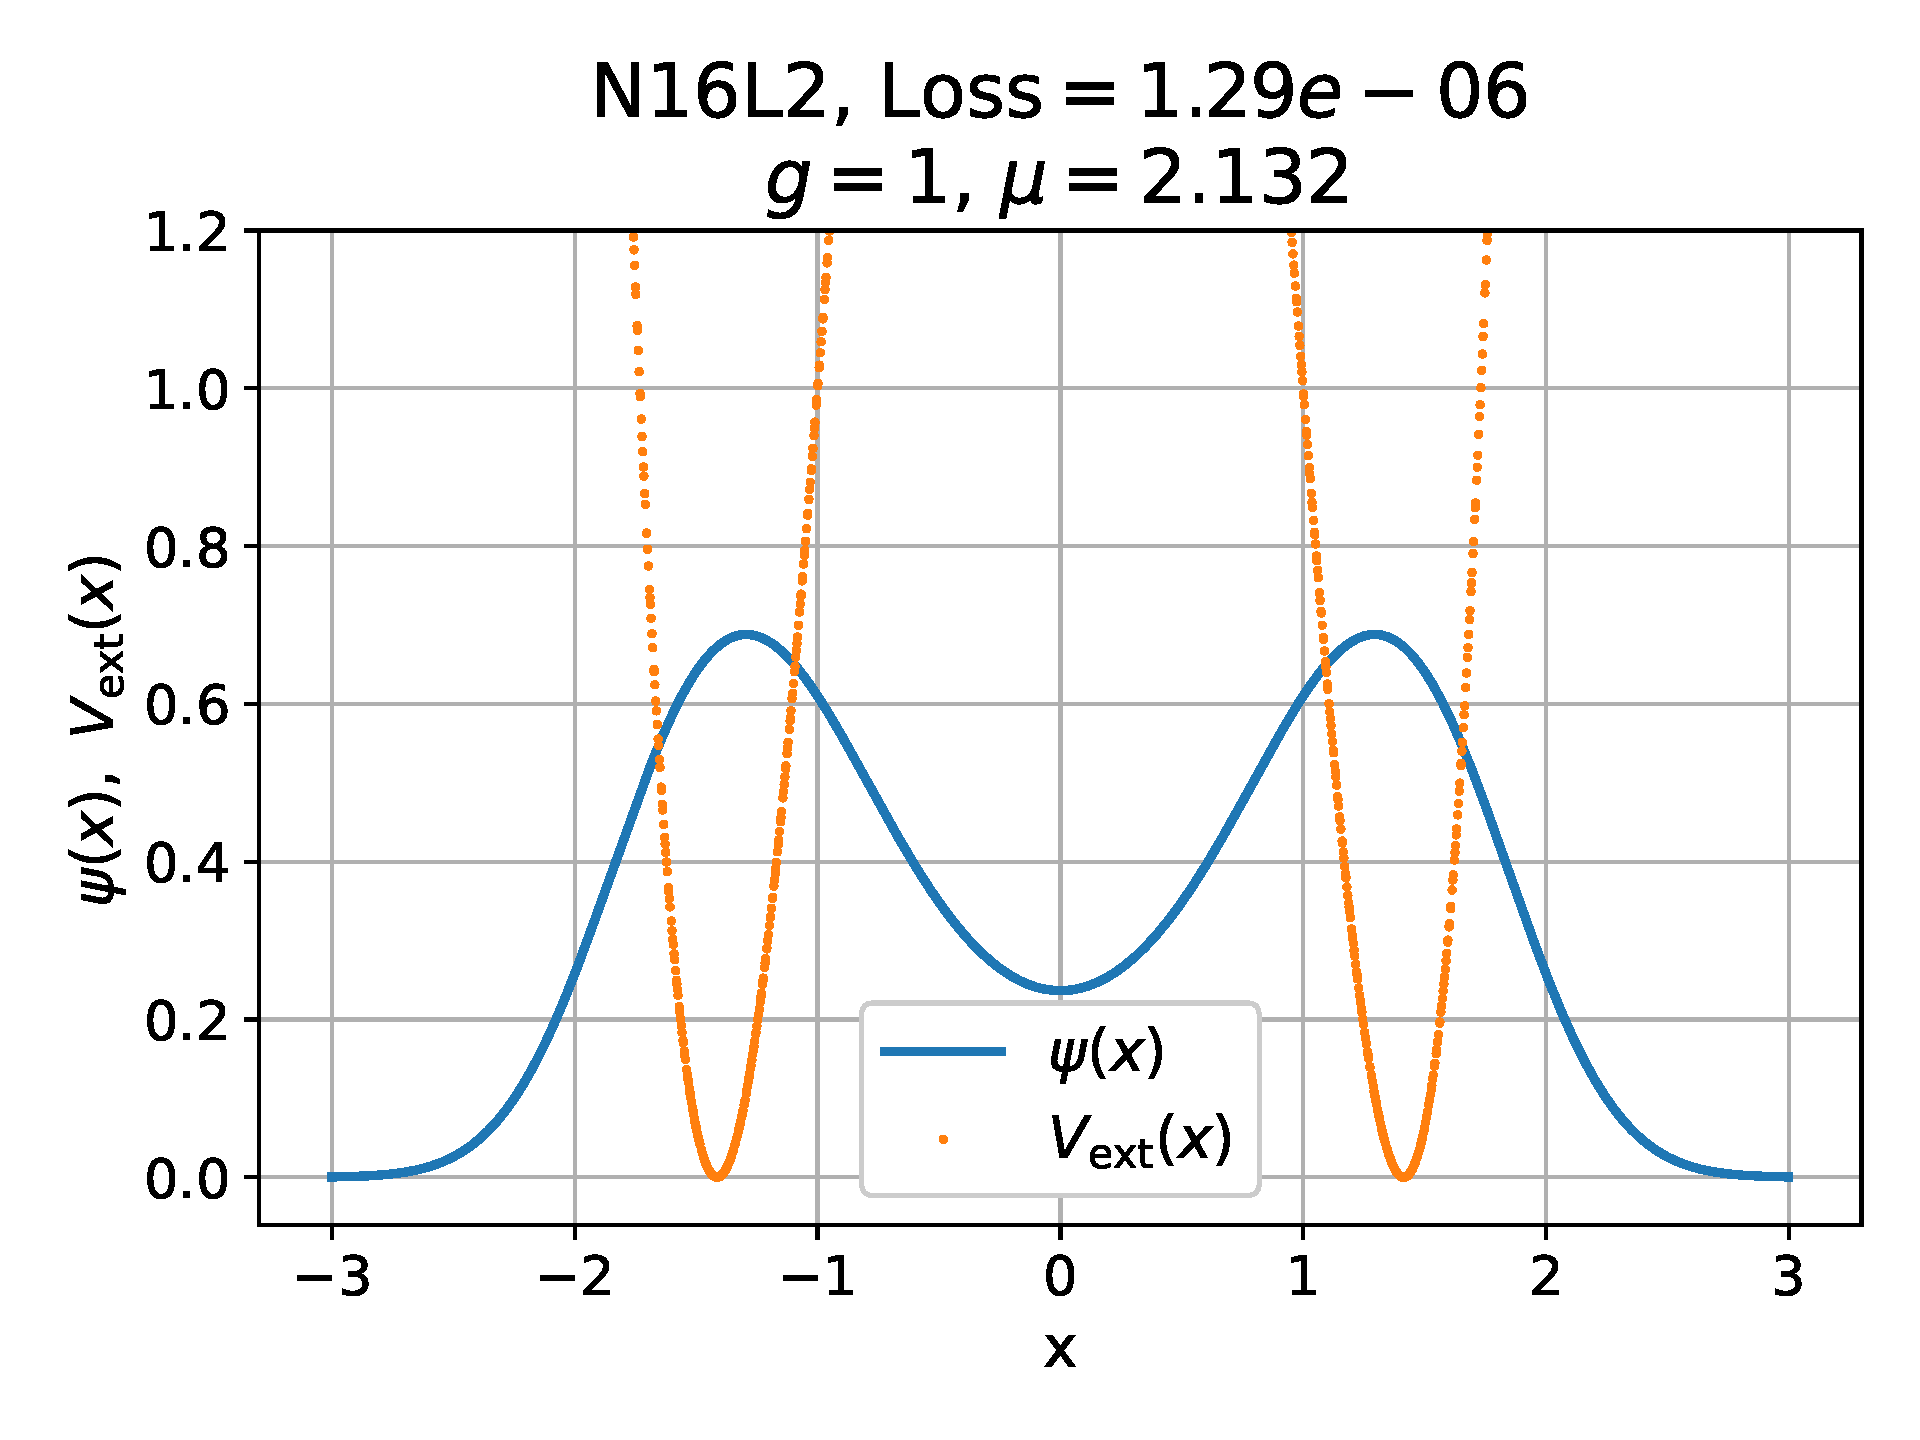
\includegraphics[width=\textwidth]{Figures/ex3_1D_N16L2_pos_g1_dw2_high_g.png}
    \caption{Starting from the NN trained at $g = 100$ in Figure
    \ref{fig:ex3_dw2_yee_g100} and optimizing it for $g = 1$ we can find the 
    ground state solution for the double well potential with $a = 2$.}
    \label{fig:ex3_dw2_yee_g1}
\end{minipage}
\hspace{0.05\textwidth}
\begin{minipage}{0.48\textwidth}
    \centering
    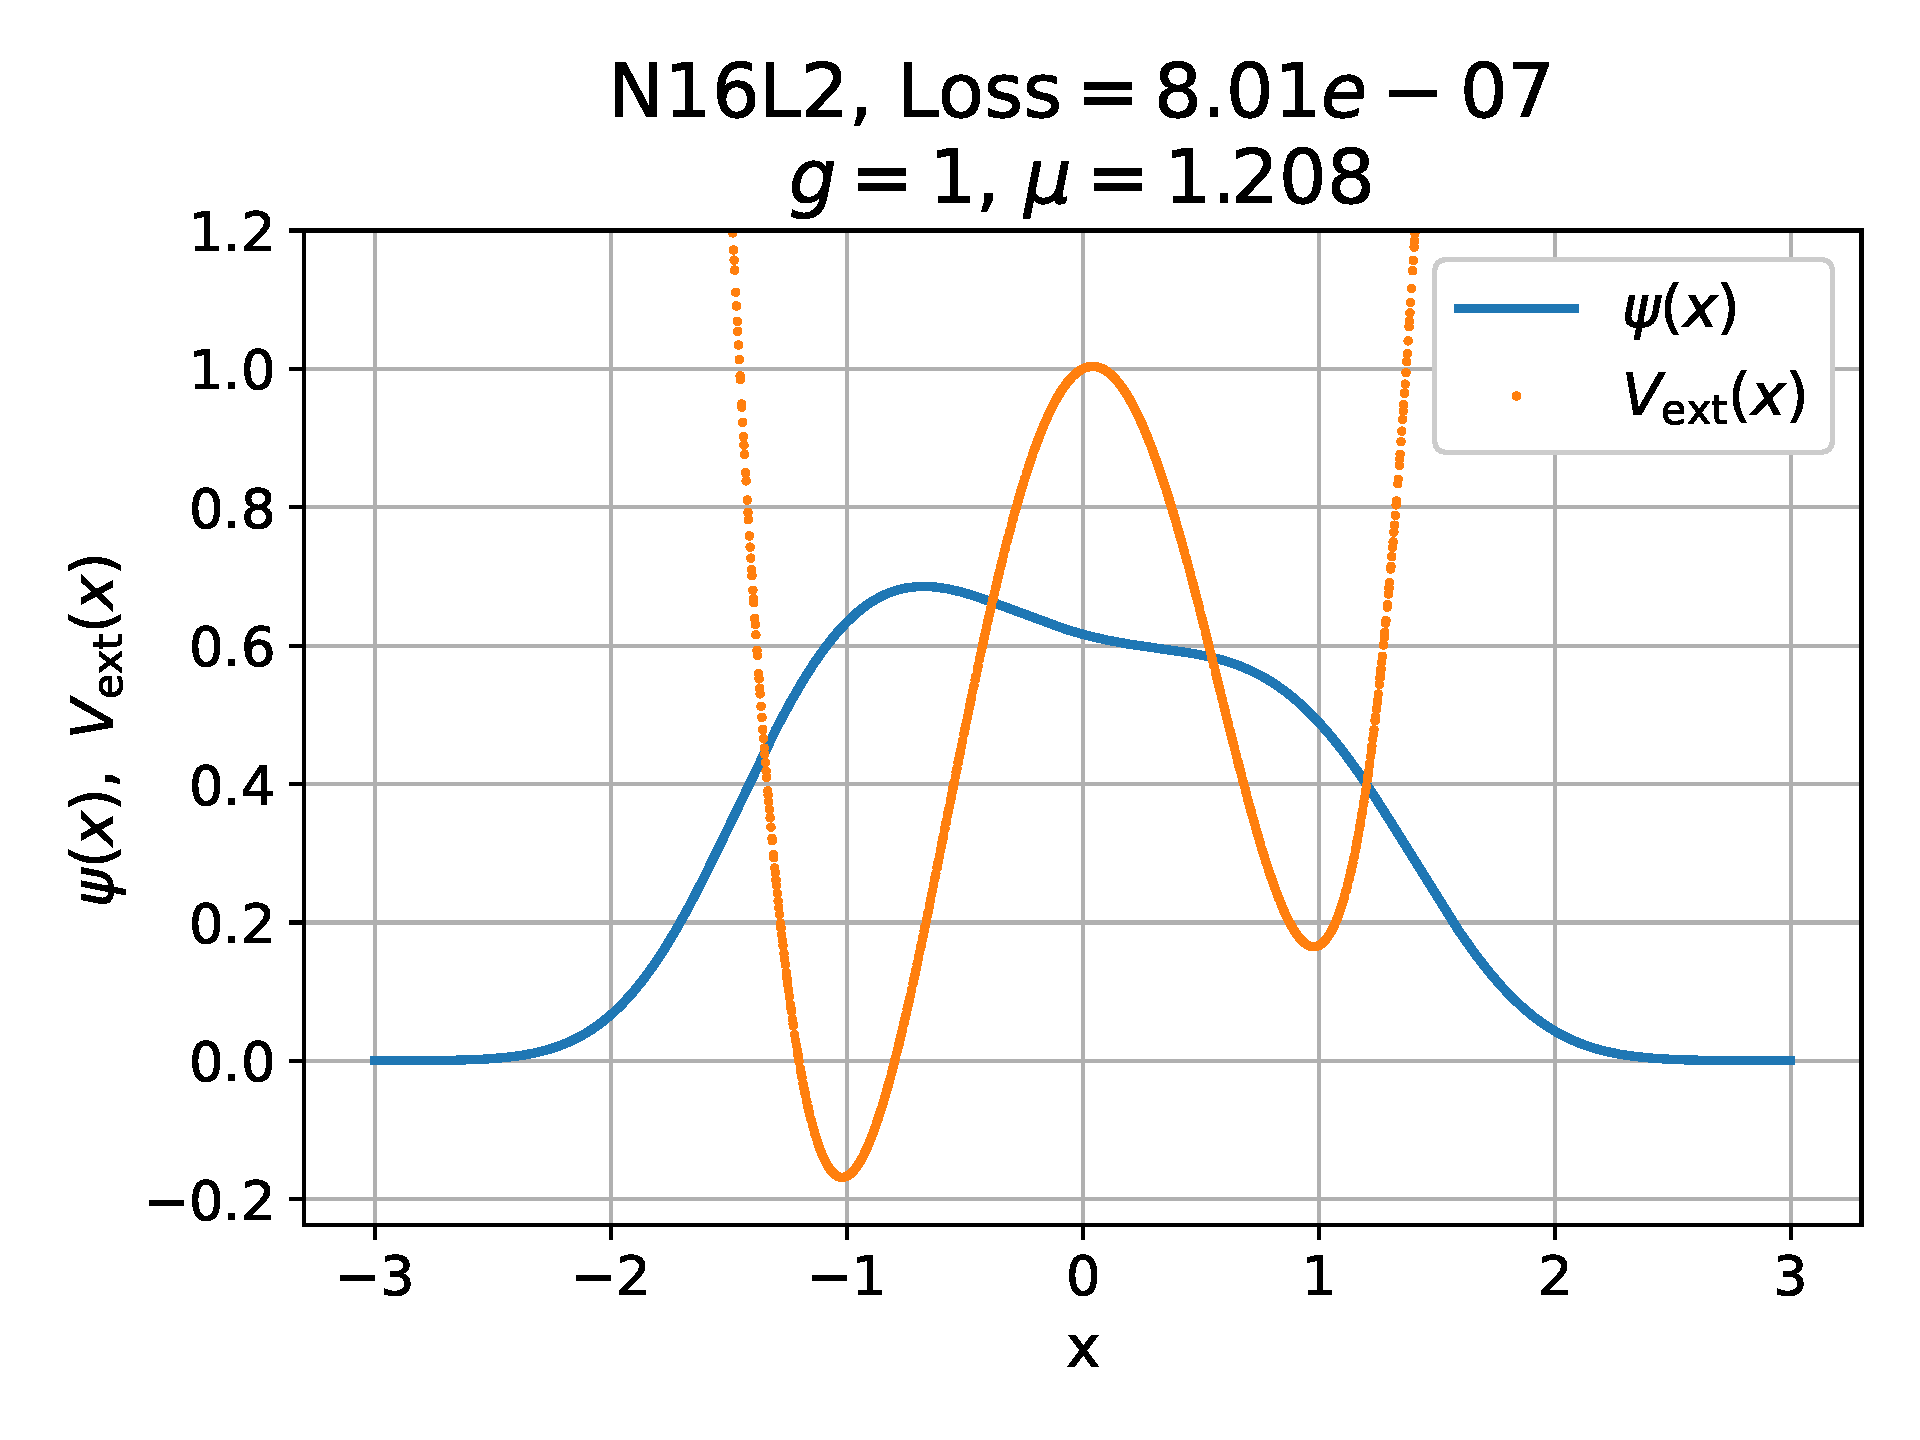
\includegraphics[width=\textwidth]{Figures/ex3_1D_N16L2_pos_g1_dw1_as6_high_g.png}
    \caption{N16L2 positive NN trained for $g = 100$ and then retrained for
    $g = 1$ with the non-symmetric double well potential from equation 
    \eqref{eq:dw_as} with $a = 1$ and $b = 6$. 
    The wave function is more localized in the left well, as expected.}
    \label{fig:ex3_dw1_as6}
\end{minipage}
\end{figure}

Finally, we can also use a non-symmetric double well potential
\begin{equation}
    V_{\rm ext}(x) = \left(x^2 - a\right)^2 + \frac{x}{b} \, .
    \label{eq:dw_as}
\end{equation}
Using $a = 1$, $b = 6$ we can apply the same method as before by first finding a
solution for $g = 100$ and then retraining the NN for $g = 1$.
The result is shown in Figure \ref{fig:ex3_dw1_as6}, where we can see that 
the wave function is more localized in the left well, as expected.

These results, obtained by first finding a solution with a high interaction
strength, can probably be found by varying the external potential instead and
slowly changing it to the final configuration.
But given that the potential can have many parameters and that later on we will
have to deal with a 2D one, using the single number $g$ to control the evolution
of the solution can be more convenient.

A different approach to address the eigenvalue problem under some approximation
is reported in Appendix \ref{app:eigenvalue}, where we find multiple eigenstates
of the problem at the same time.


\subsection{2D Double Well} \label{sec:2d_double_well}

We now extend the problem to 2D, where the NN takes $(x, y)$ as inputs.
The loss is defined as
\begin{equation}
\begin{aligned}
    \mathcal L &= \mathcal L_{\rm PDE} + \mathcal L_{\rm BC} 
        + 10 \, \mathcal L_{\rm norm} \\
    \mathcal L_{\rm PDE} &= \frac{1}{N_f} \sum_{i=1}^{N_f}
        \left( -\frac{1}{2} \dv[2]{\phi(r_i)}{r} + \frac{1}{2} r_i^2 \phi(r_i) 
        + Na \left(\frac{\phi(r_i)}{r_i}\right)^2 \phi(r_i)
        - \mu \phi(r_i) \right)^2 \\
    \mathcal L_{\rm BC} &= \frac{1}{N_b} \sum_{i=1}^{N_b} 
        \left( \phi(r_i) \right)^2 \\
    \mathcal L_{\rm norm} &= \left( \frac{R - \epsilon}{N}
        \sum_{i = 1}^N \phi(r_i)^2  - 1 \right)^2 \, .
\end{aligned}
\label{eq:2D_loss}
\end{equation}
For the harmonic potential $V_{\rm ext}(x, y) = \frac{1}{2}(x^2 + y^2)$ with
$g = 1$ the optimizer converges without difficulty, and the results are shown
in Figure \ref{fig:ex3_2D_N32L3_g1_harmonic}.
\begin{figure}[h!]
    \centering
    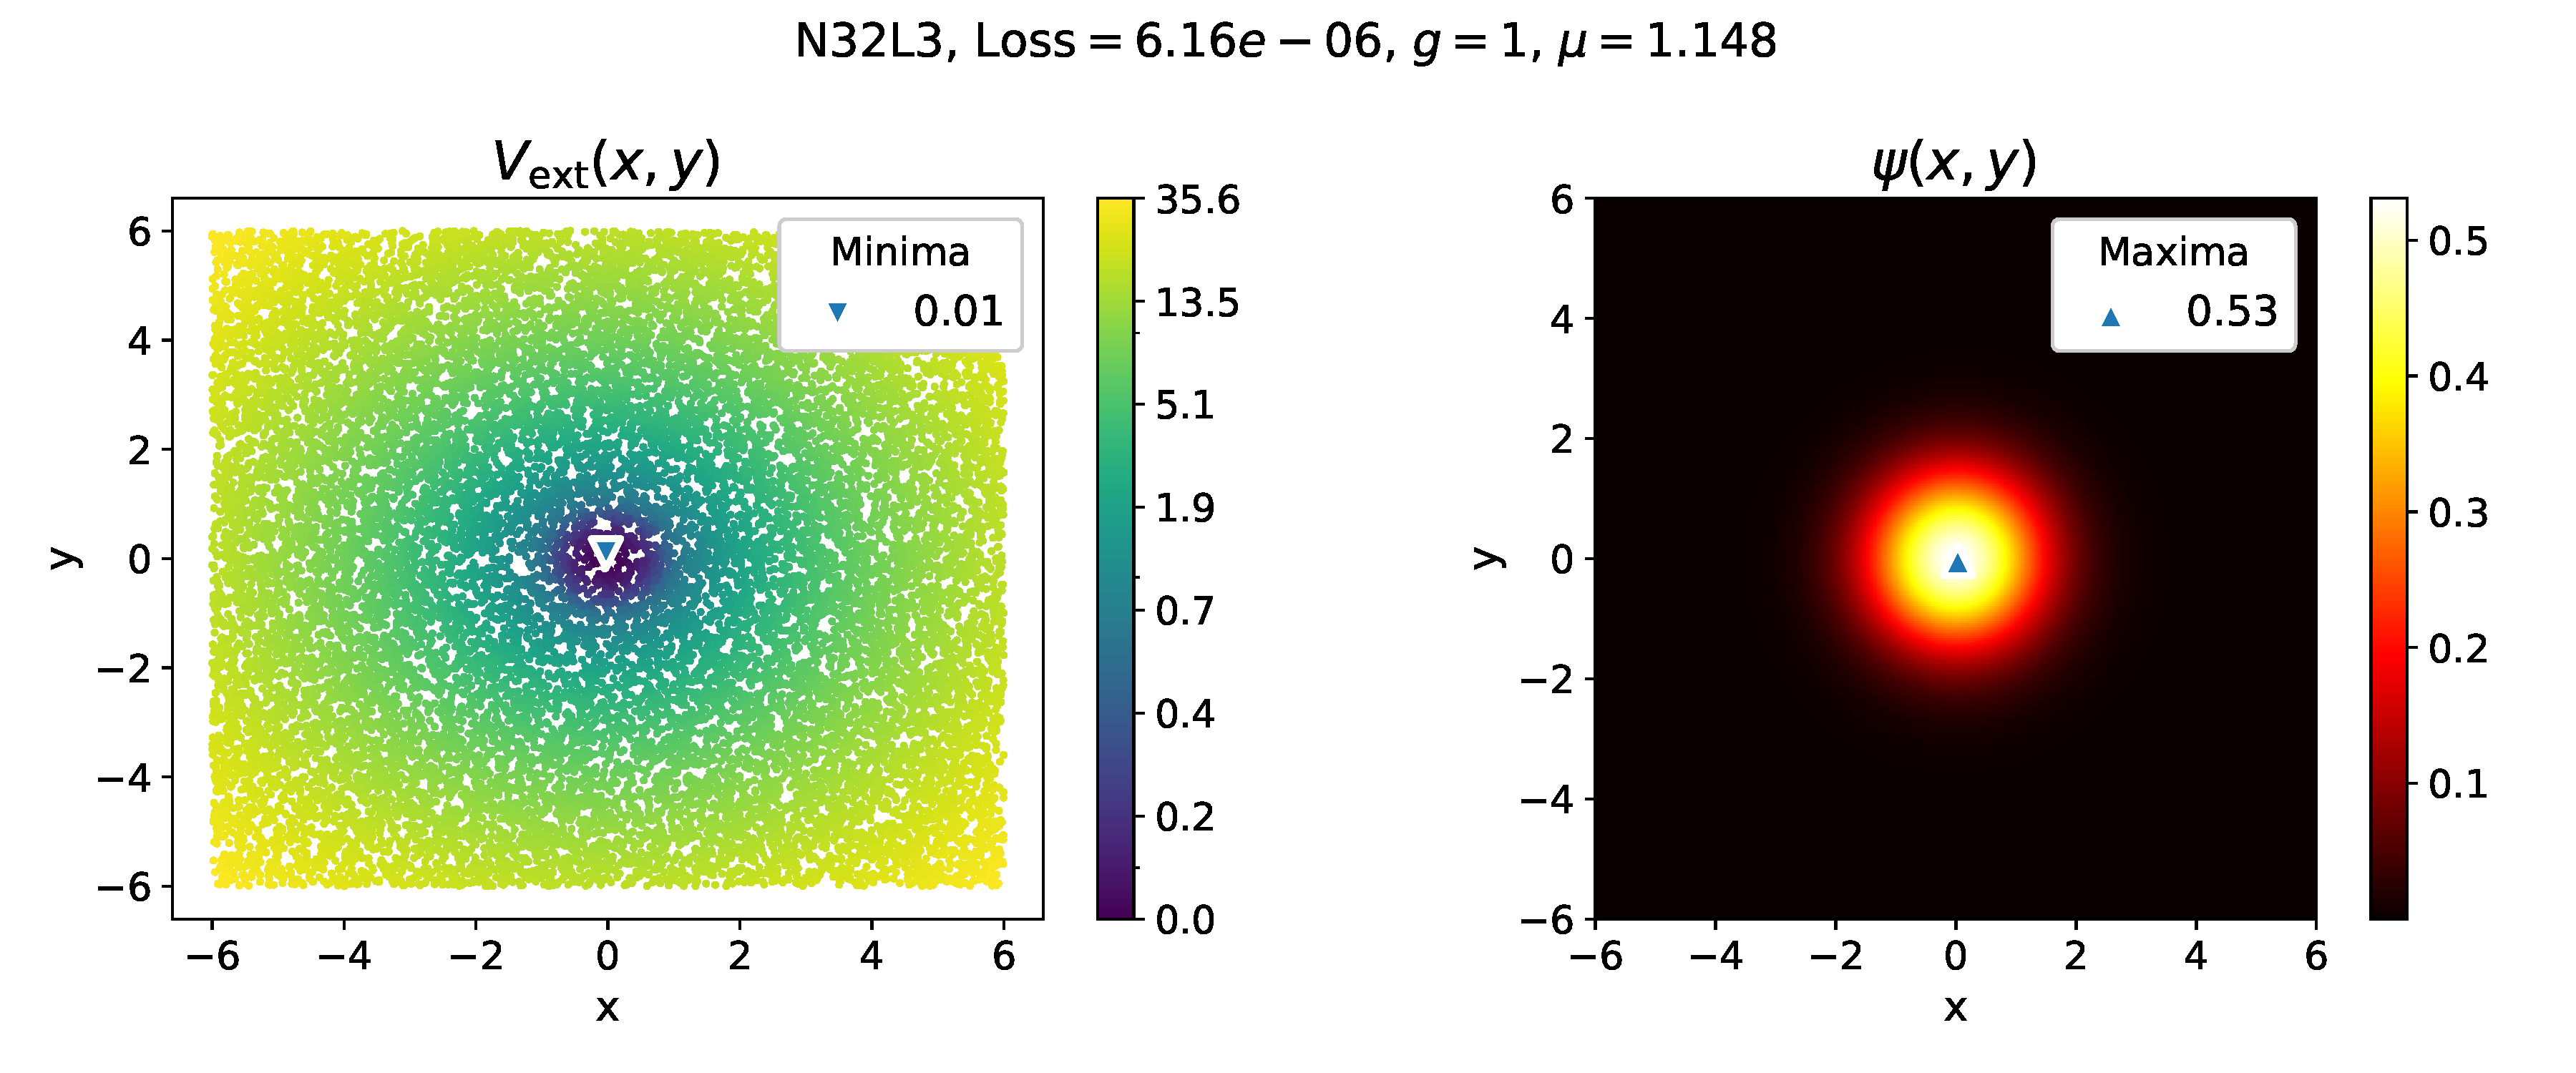
\includegraphics[width=\textwidth]{Figures/ex3_2D_N32L3_g1_harmonic.png}
    \caption{Results for the 2D GPE with a harmonic potential and $g = 1$ using a NN
    with N32L3. Gaussian initialization was used to help the optimizer.}
    \label{fig:ex3_2D_N32L3_g1_harmonic}
\end{figure}

When trying a double well potential (even a symmetric one) we find ourselves in
the same situation encountered in the 2D case, where, even with a gaussian
initialization and a positivity constraint on the NN, the optimizer is content
to only grow the wave function in one of the wells (no matter which one).
We are therefore forced to use the same strategy described at the end of section
\ref{sec:1d_double_well}: we first find a solution with a high interaction
strength, which allows the wave function to spread over both wells, and then 
retrain the NN for smaller values of $g$.

We can immediately look at a non-symmetric double well potential
\begin{equation}
    V_{\rm ext}(x, y) = x^4 + \left(y^2 - 2\right)^2 + \frac{y}{6} + xy \, .
    \label{eq:dw_as_2d}
\end{equation}

We first train a N32L3 NN for $g = 40$, the result is shown in Figure
\ref{fig:ex3_2D_N32L3_g40_dw2_as6_gauss}, and then retrain it for $g = 1$, the
result is shown in Figure \ref{fig:ex3_2D_N32L3_g1_dw2_as6_high_g}.
We can appreciate how the wave function is more localized in the lower well, 
while still showing a significant density in the higher well as well.

\begin{figure}[h!!!]
    \centering
    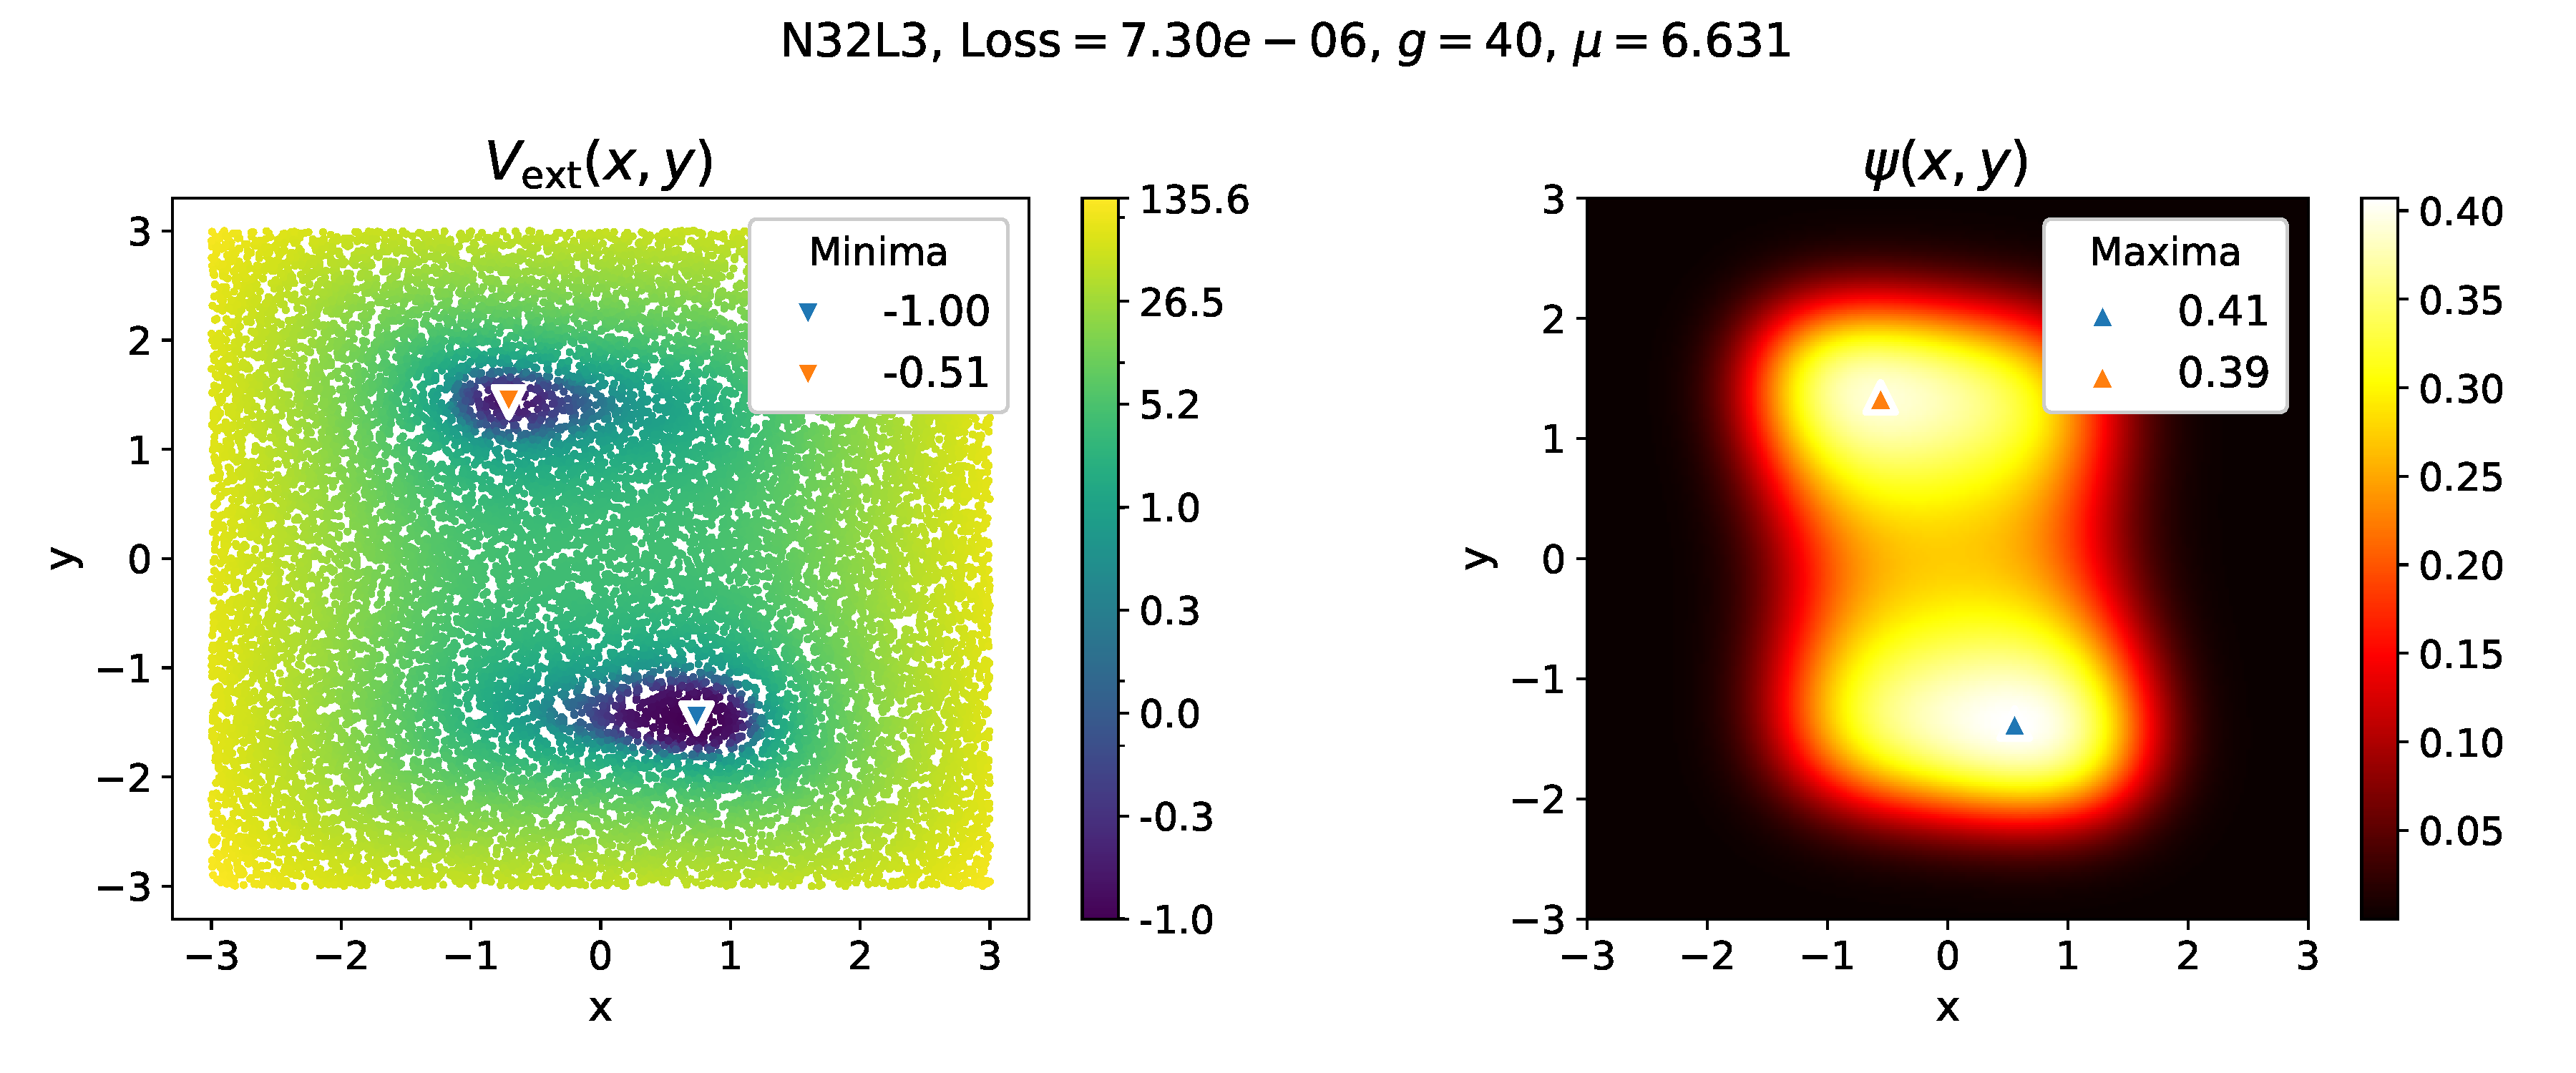
\includegraphics[width=\textwidth]
    {Figures/ex3_2D_N32L3_g40_dw2_as6_gauss.png}
    \caption{2D GPE with the asymmetric double well potential from equation
    \eqref{eq:dw_as_2d} and $g = 40$, using a NN with N32L3. At high interaction
    strength the wave function easily spreads over both wells.}
    \label{fig:ex3_2D_N32L3_g40_dw2_as6_gauss}
\end{figure}
\begin{figure}[h!!!]
    \centering
    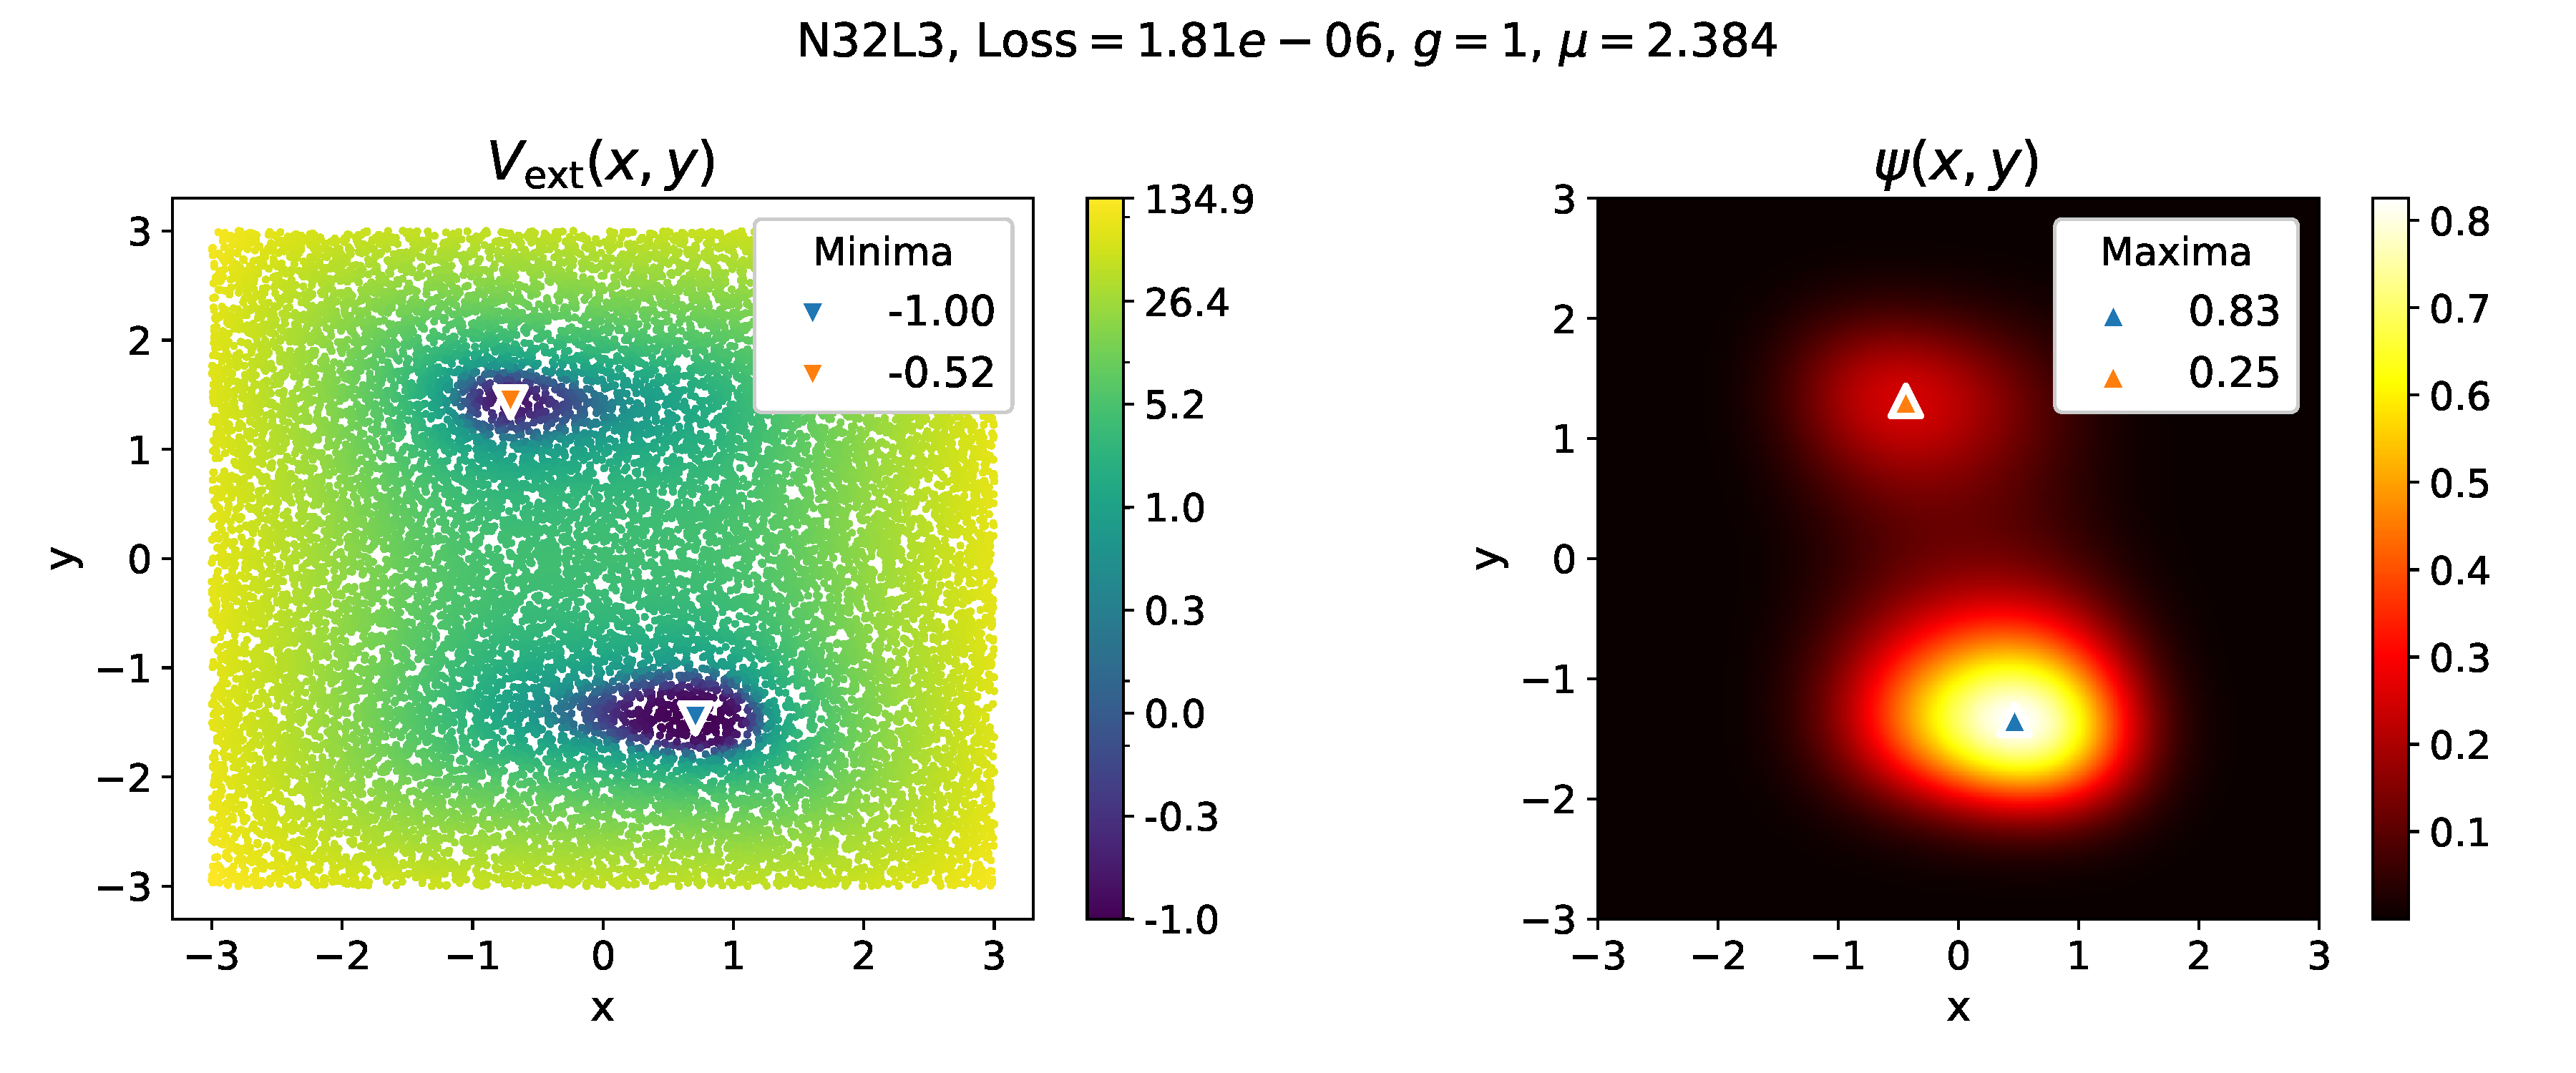
\includegraphics[width=\textwidth]
    {Figures/ex3_2D_N32L3_g1_dw2_as6_high_g.png}
    \caption{The NN of Figure \ref{fig:ex3_2D_N32L3_g40_dw2_as6_gauss} retrained
    for $g = 1$.
    The wave function is now more localized in the lower well of the asymmetric
    potential, as expected.}
    \label{fig:ex3_2D_N32L3_g1_dw2_as6_high_g}
\end{figure}




\newpage
\subsection{A Modulated Mexican Hat} \label{sec:complex_2d_traps}
Further testing the robustness of the PINN approach, we consider a highly
structured two-dimensional trap obtained by combining a radial ``Mexican-hat''
confinement with an angular modulation,
\begin{equation}
    V_{\rm ext}(x,y)
    = \bigl(x^2+y^2-2\bigr)^2 + \mathcal E \cos (5 \theta),
    \qquad
    \theta = \mathrm{atan2}(y,x)\,,
    \label{eq:weird_potential}
\end{equation}
where the first term confines the density on a ring of radius
$r_0=\sqrt{2}$, while the second term breaks rotational symmetry and produces
five preferred angular minima along the ring.
Our goal is to solve the GPE with $g=1$ at two values of the modulation 
strength: $\mathcal E = 0.4$ and $\mathcal E = 10$.
Considering the potential landscape we also increased the number of sample 
points to $N_f = 40000$, the loss term $\mathcal L$ remains otherwise the 
same as in equation \eqref{eq:2D_loss}.

The corresponding solutions are shown in Figures
\ref{fig:ex3_2D_N32L3_g1_crazy_eps0.4} and
\ref{fig:ex3_2D_N32L3_g1_crazy_eps10}. 
In both cases the network accurately
reproduces the angular density modulations induced by the potential.
For $\mathcal E = 0.4$ the trap is only weakly corrugated, and the training
procedure was quite straightforward, it was sufficient to solve the problem
with $g = 40$ and then retrain the network for $g = 1$ to find the final 
solution.
For $\mathcal E = 10$ on the other end, the trap is strongly corrugated and the 
wave function is highly localized in the angular minima, which made the
optimization challenging.

\begin{figure}[h!]
    \centering
    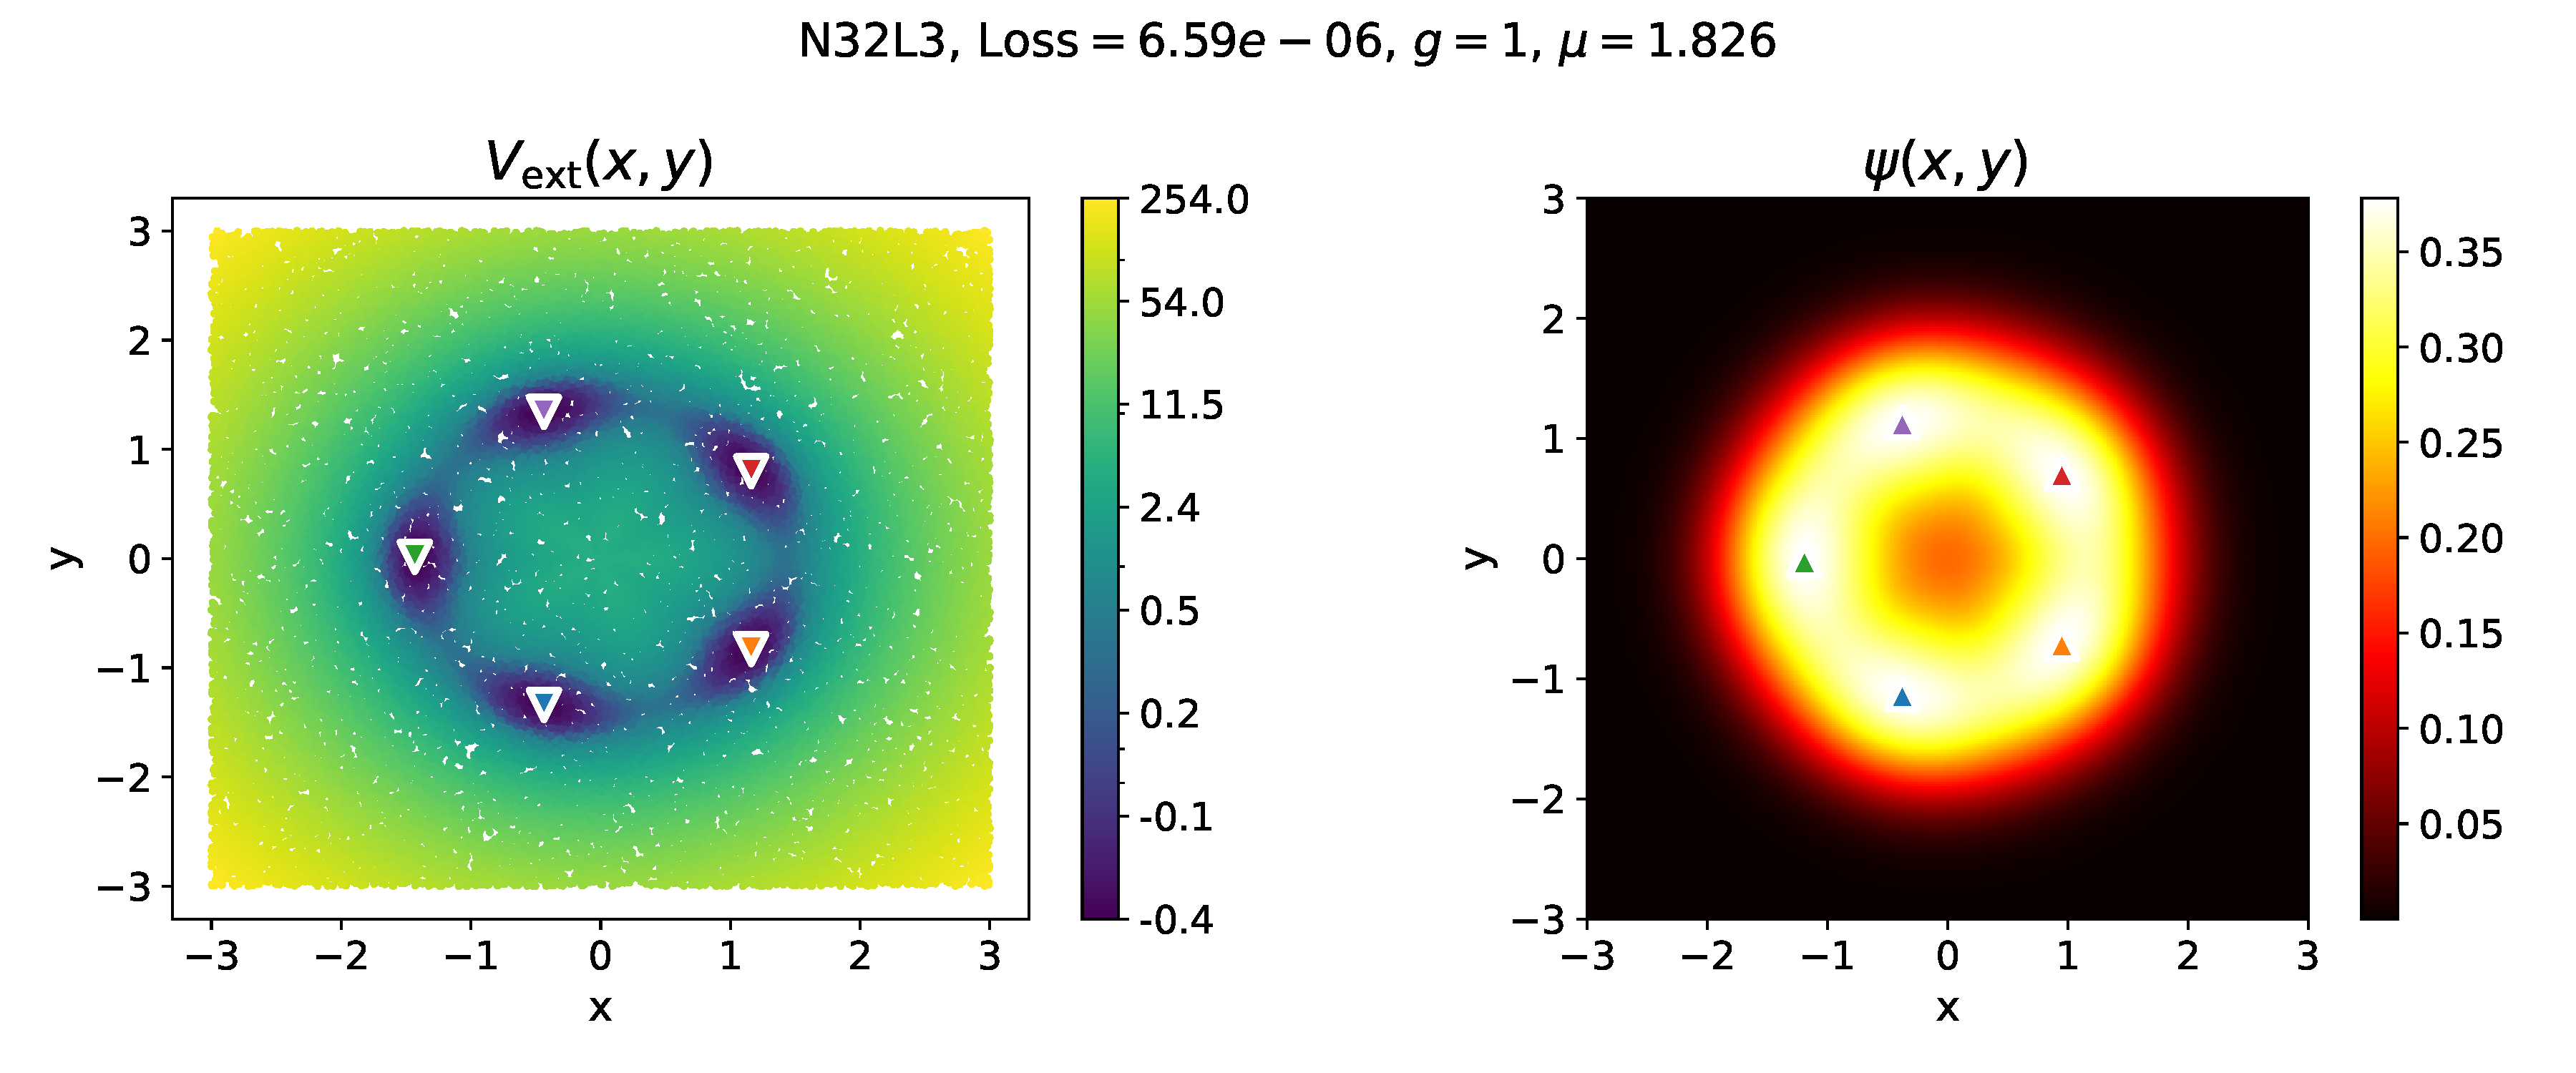
\includegraphics[width=\textwidth]
    {Figures/ex3_2D_N32L3_g1_crazy_a2.0_eps0.4_n5_high_g.png}
    \caption{Stationary solution of the 2D GPE with the potential
    \eqref{eq:weird_potential} at $\mathcal E=0.4$ and $g=1$, obtained with a
    N32L3 PINN. 
    The wave function follows the five-fold modulation of the external trap 
    along the ring.
    The potential minima are denoted with a $\blacktriangledown$ symbol and
    are all $V_{\rm min} \simeq 0.40$ deep, while the maxima of the wave-function
    are denoted with a $\blacktriangle$ symbol and are all 
    $\psi_{\rm max} \simeq 0.38$ high.}
    \label{fig:ex3_2D_N32L3_g1_crazy_eps0.4}
\end{figure}

\begin{figure}[h!]
    \centering
    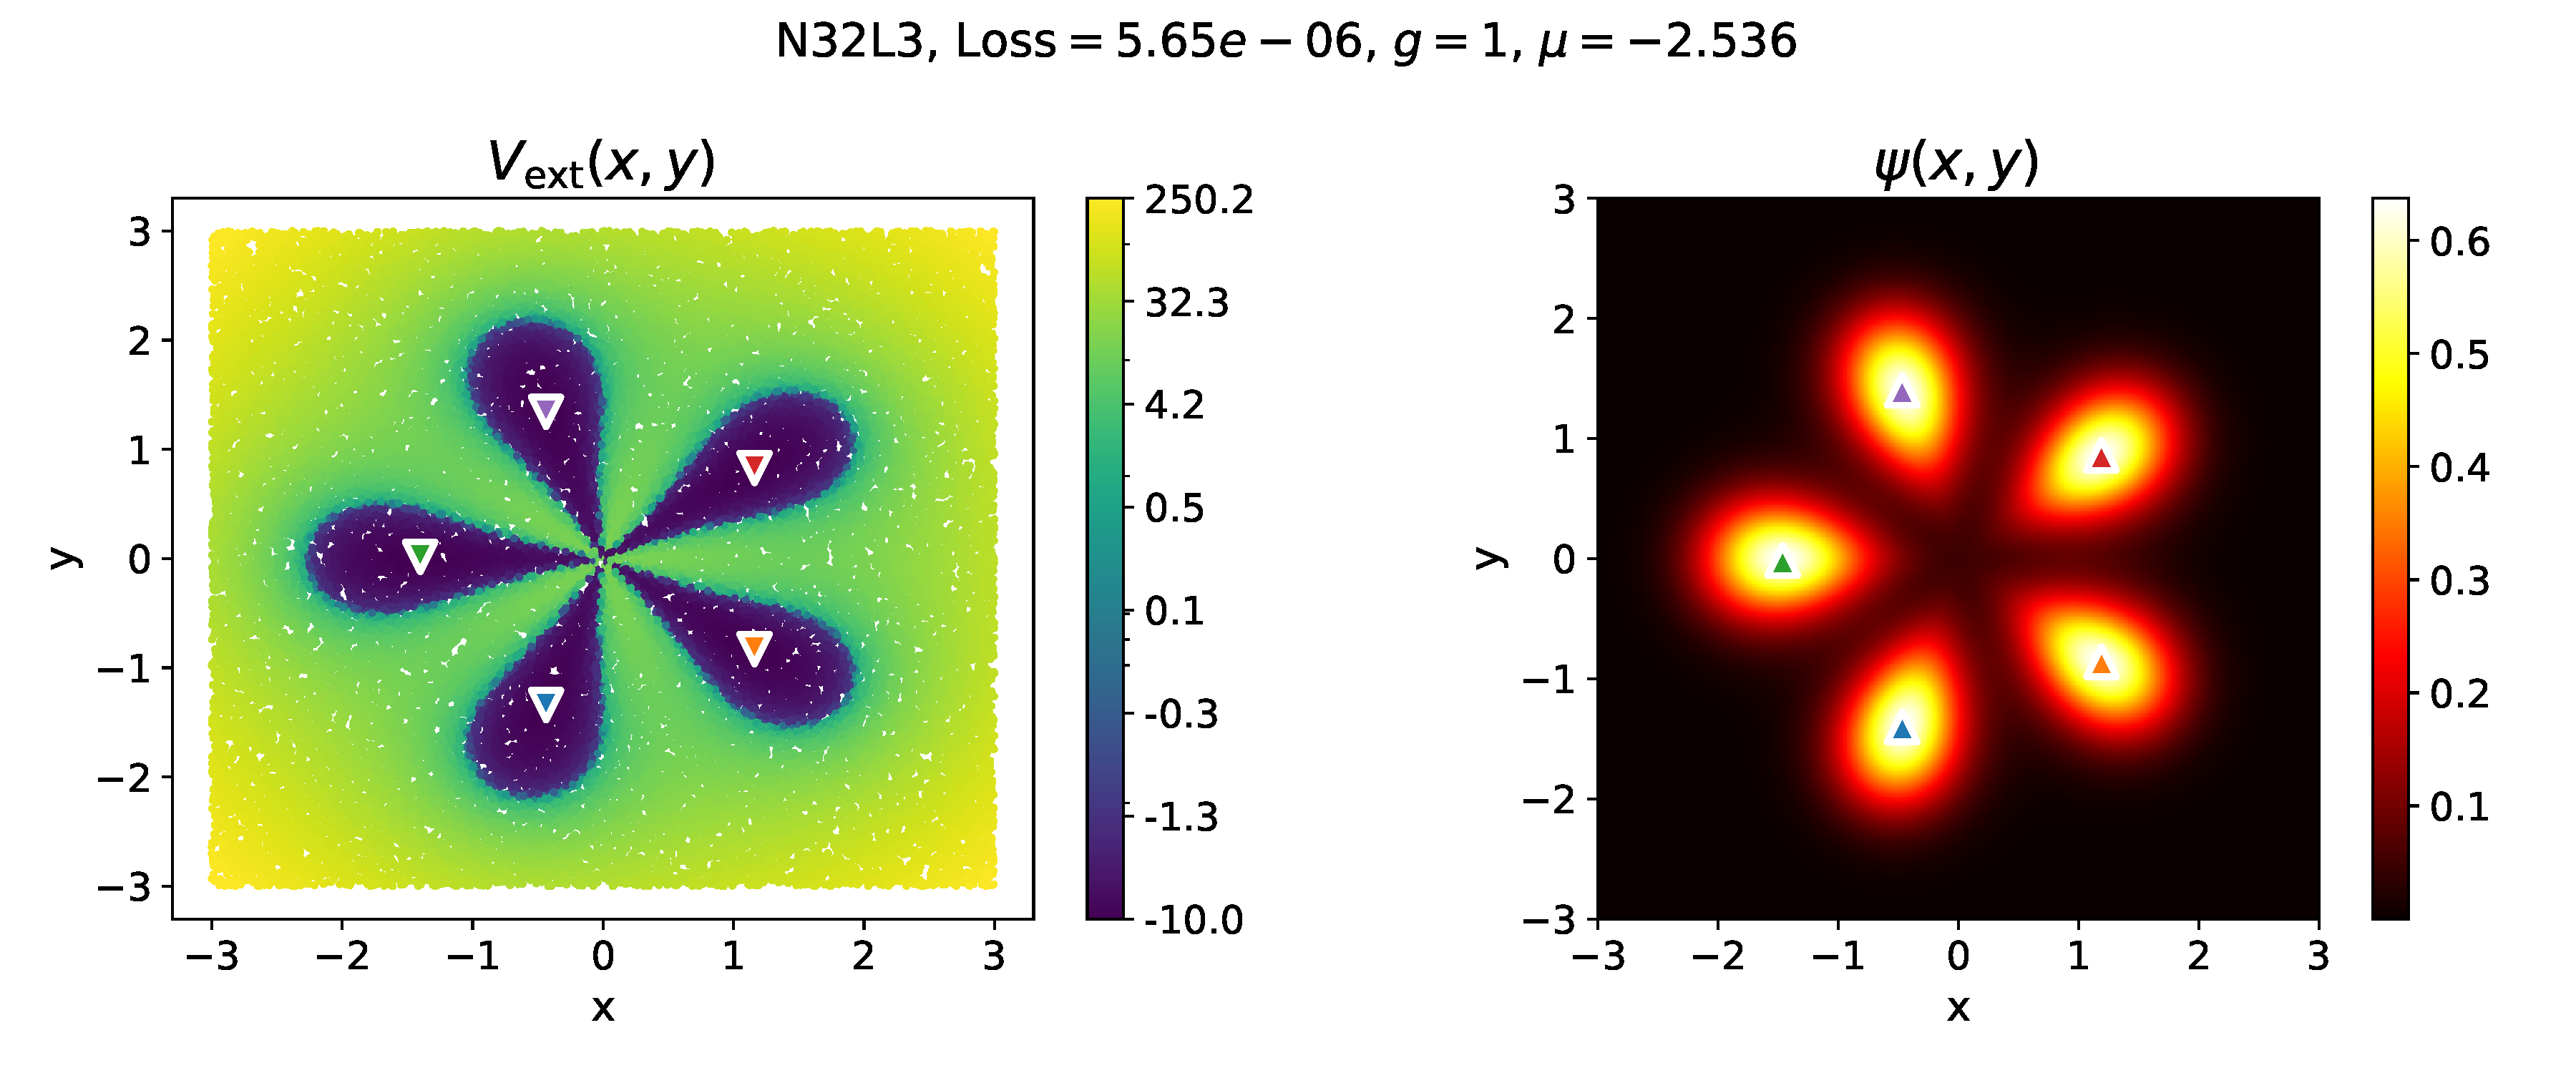
\includegraphics[width=\textwidth]
    {Figures/ex3_2D_N32L3_g1_crazy_a2.0_eps10.0_n5_var.png}
    \caption{Same as Figure~\ref{fig:ex3_2D_N32L3_g1_crazy_eps0.4}, but with a
    much stronger angular corrugation, $\mathcal E = 10$ meaning that the
    angular barriers are $\Delta V \simeq 20$ high.
    Even in this stiff regime the PINN converges to a solution that captures the
    sharp modulation and the increased localization in the angular minima.
    The potential minima are denoted with a $\blacktriangledown$ symbol and
    are all $V_{\rm min} \simeq -10$ deep, while the maxima of the wave-function
    are denoted with a $\blacktriangle$ symbol and are all 
    $\psi_{\rm max} \simeq 0.64$ high.}
    \label{fig:ex3_2D_N32L3_g1_crazy_eps10}
\end{figure}

To obtain the result in Figure \ref{fig:ex3_2D_N32L3_g1_crazy_eps0.4}, it was
inconvenient to find an interaction strength $g$ high enough to overcome the 
angular barriers that have a $\Delta V \simeq 20$, consequently we leveraged the
situation to see if modifying the potential would work as well.
We started from the NN obtained in Figure \ref{fig:ex3_2D_N32L3_g1_crazy_eps0.4}
with $\mathcal E = 0.4$ and $g = 1$, and gradually increased $\mathcal E$ until
we reached the target value of $\mathcal E = 10$.
At each step we let the optimizer run up to convergence (that was always in the
order of $10^{-5}$) before increasing $\mathcal E$ again.
It was crucial to use small increments of $\mathcal E$, otherwise we could 
observe the optimizer getting stuck at a loss of $\sim 10^{-4}$, and the
solution dropping a couple of the density peaks entirely.
But in the end, thanks to a combination of a warm high $g$ start and a slow
modification of the potential we could reach the final solution.

An even more challenging potential with more wells is shown in Appendix
\ref{app:spread_out_potential}.




\newpage
\section{Vortex Solutions} \label{sec:vortex}
\begin{figure}[h!]
    \centering
    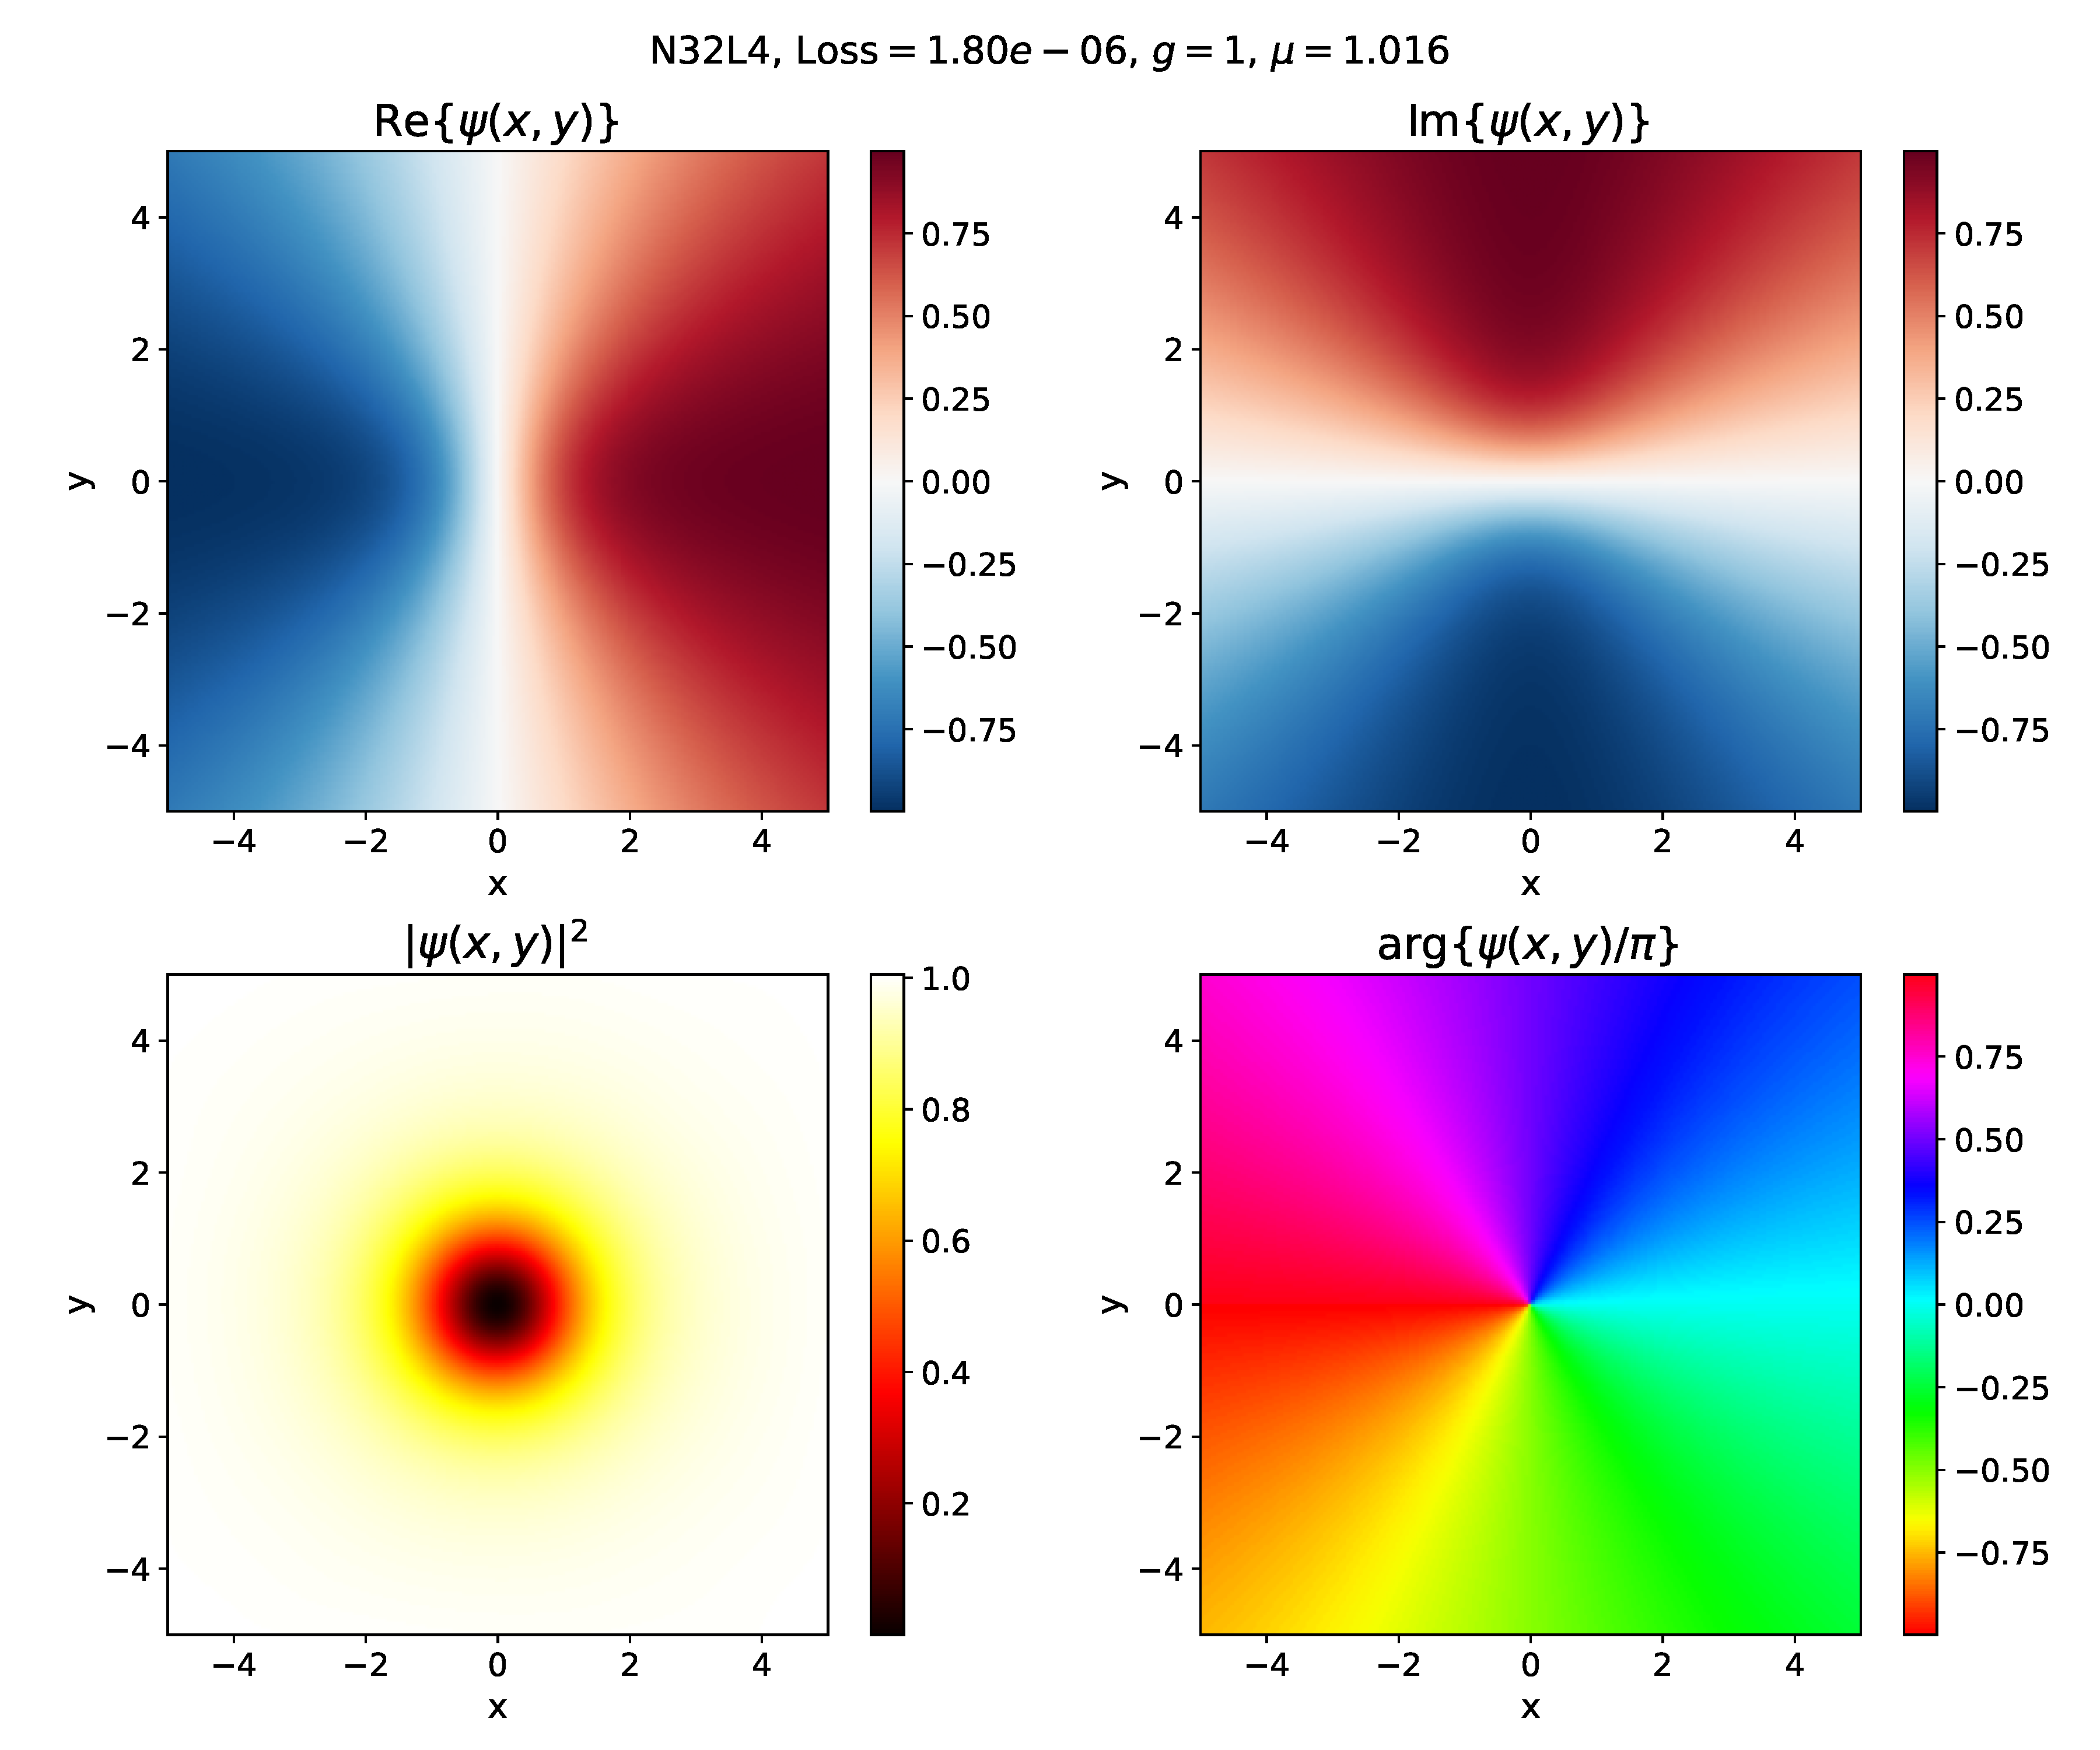
\includegraphics[width=\textwidth]{Figures/ex4_N32L4_PINN_Na1.0_x-5.00_-5.00-5.00_5.00_l1_full.png}
    \caption{Vortex solution of the 2D GPE with $g = 1$ and winding number $m = 1$,
    obtained with a NN with N32L4.}
    \label{fig:vortex_l1}
\end{figure}
As a final application we search for quantized vortex solutions of the
stationary GPE in 2D without an external potential,
\begin{equation}
    -\frac{1}{2}\nabla^2\psi
    + \left(g|\psi|^2 - \mu\right)\psi = 0\,.
    \label{eq:vortex_gpe}
\end{equation}
A vortex of winding number $m$ is a solution of the form
\begin{equation}
    \psi(r,\theta) = f(r)\,e^{im\theta}\,,
    \label{eq:vortex_ansatz}
\end{equation}
where $f(r)\geq 0$ is a real radial profile that vanishes at the origin,
forming the vortex core, and saturates to a constant density at large $r$.
Such a state carries a quantized circulation and a phase that winds $m$
times around the core.

We represent the complex wave function with the same two-output NN used in
Section~\ref{sec:gpe_time},
\begin{equation*}
    \mathcal{N}(x,y) = \bigl[u(x,y),\;v(x,y)\bigr]\,,
    \qquad \psi = u + iv\,.
\end{equation*}
Separating real and imaginary parts of equation~\eqref{eq:vortex_gpe}
and denoting $|\psi|^2 = u^2 + v^2$, we obtain the coupled system
\begin{align*}
    f_u &\;\equiv\;
        -\frac{1}{2}\nabla^2 u
        + \bigl(g|\psi|^2 - \mu\bigr)\,u
        \;=\; 0\,,
    f_v &\;\equiv\;
        -\frac{1}{2}\nabla^2 v
        + \bigl(g|\psi|^2 - \mu\bigr)\,v
        \;=\; 0\,.
\end{align*}

Considering that we are looking for an excited state with a specific angular
momentum, the boundary conditions play a crucial role as we need to rule out
the trivial solution where $\psi$ is a constant.
On the boundary $\partial\mathcal{D}$ we directly impose the phase winding
from the ansatz~\eqref{eq:vortex_ansatz} with unit amplitude,
\begin{align*}
    u(x,y)\big|_{\partial\mathcal{D}} &= \cos(m\theta) 
    = \Re \left\{ \left(\frac{x + iy}{\sqrt{x^2+y^2}} \right)^m \right\} \\
    v(x,y)\big|_{\partial\mathcal{D}} &= \sin(m\theta) 
    = \Im \left\{ \left(\frac{x + iy}{\sqrt{x^2+y^2}} \right)^m \right\}\\
\end{align*}
These conditions fix the winding number while leaving the interior amplitude
free to relax and impose an asymptotically constant density of 
$|\psi|^2 \approx 1$.
Considering equation \eqref{eq:vortex_gpe} when $|\psi|^2$ is constant we have
immediately that $\psi = \sqrt{\frac{\mu}{g}}$ for the solution to be
consistent, so we expect the chemical potential $\mu$ to be close to $g$ for the
solution to be correct.

The total loss is
\begin{align}
    \mathcal{L} &= \mathcal{L}_{\rm PDE} + \mathcal{L}_{\rm BC}\,,
    \label{eq:vortex_loss}\\[4pt]
    \mathcal{L}_{\rm PDE} &= \frac{1}{N}\sum_{i=1}^{N}
        \Bigl[f_u(x_i,y_i)^2 + f_v(x_i,y_i)^2\Bigr]\,,
    \label{eq:vortex_lpde}\\[4pt]
    \mathcal{L}_{\rm BC} &= \frac{1}{N_b}\sum_{i=1}^{N_b}
        \Bigl[\bigl(u(x_i,y_i)-\cos(m\theta_i)\bigr)^2
             +\bigl(v(x_i,y_i)-\sin(m\theta_i)\bigr)^2\Bigr]\,,
    \label{eq:vortex_lbc}
\end{align}
where $N=20000$ collocation points are sampled from the interior with LHS,
$N_b=400$ points are distributed with LHS along $\partial\mathcal{D}$, and the
chemical potential $\mu$ is a trainable parameter.

Figure \ref{fig:vortex_l1} shows the results for a vortex with winding number 
$m = 1$ and interaction strength $g = 1$ obtained with a NN with N32L4, where 
the vortex core and the expected phase winding are clearly visible.
Increasing the winding number to $m = 3$ results in a larger vortex core, as
shown in Figure \ref{fig:vortex_l3}, which is consistent with the fact that
the centrifugal barrier increases with $m$.

Finally, increasing the interaction strength to $g = 10$ makes the vortex
smaller.
So we could find a solution with a higher winding number $m = 6$ without 
enlarging the domain, as shown in Figure \ref{fig:vortex_l6}.
\begin{figure}[h!]
    \centering
    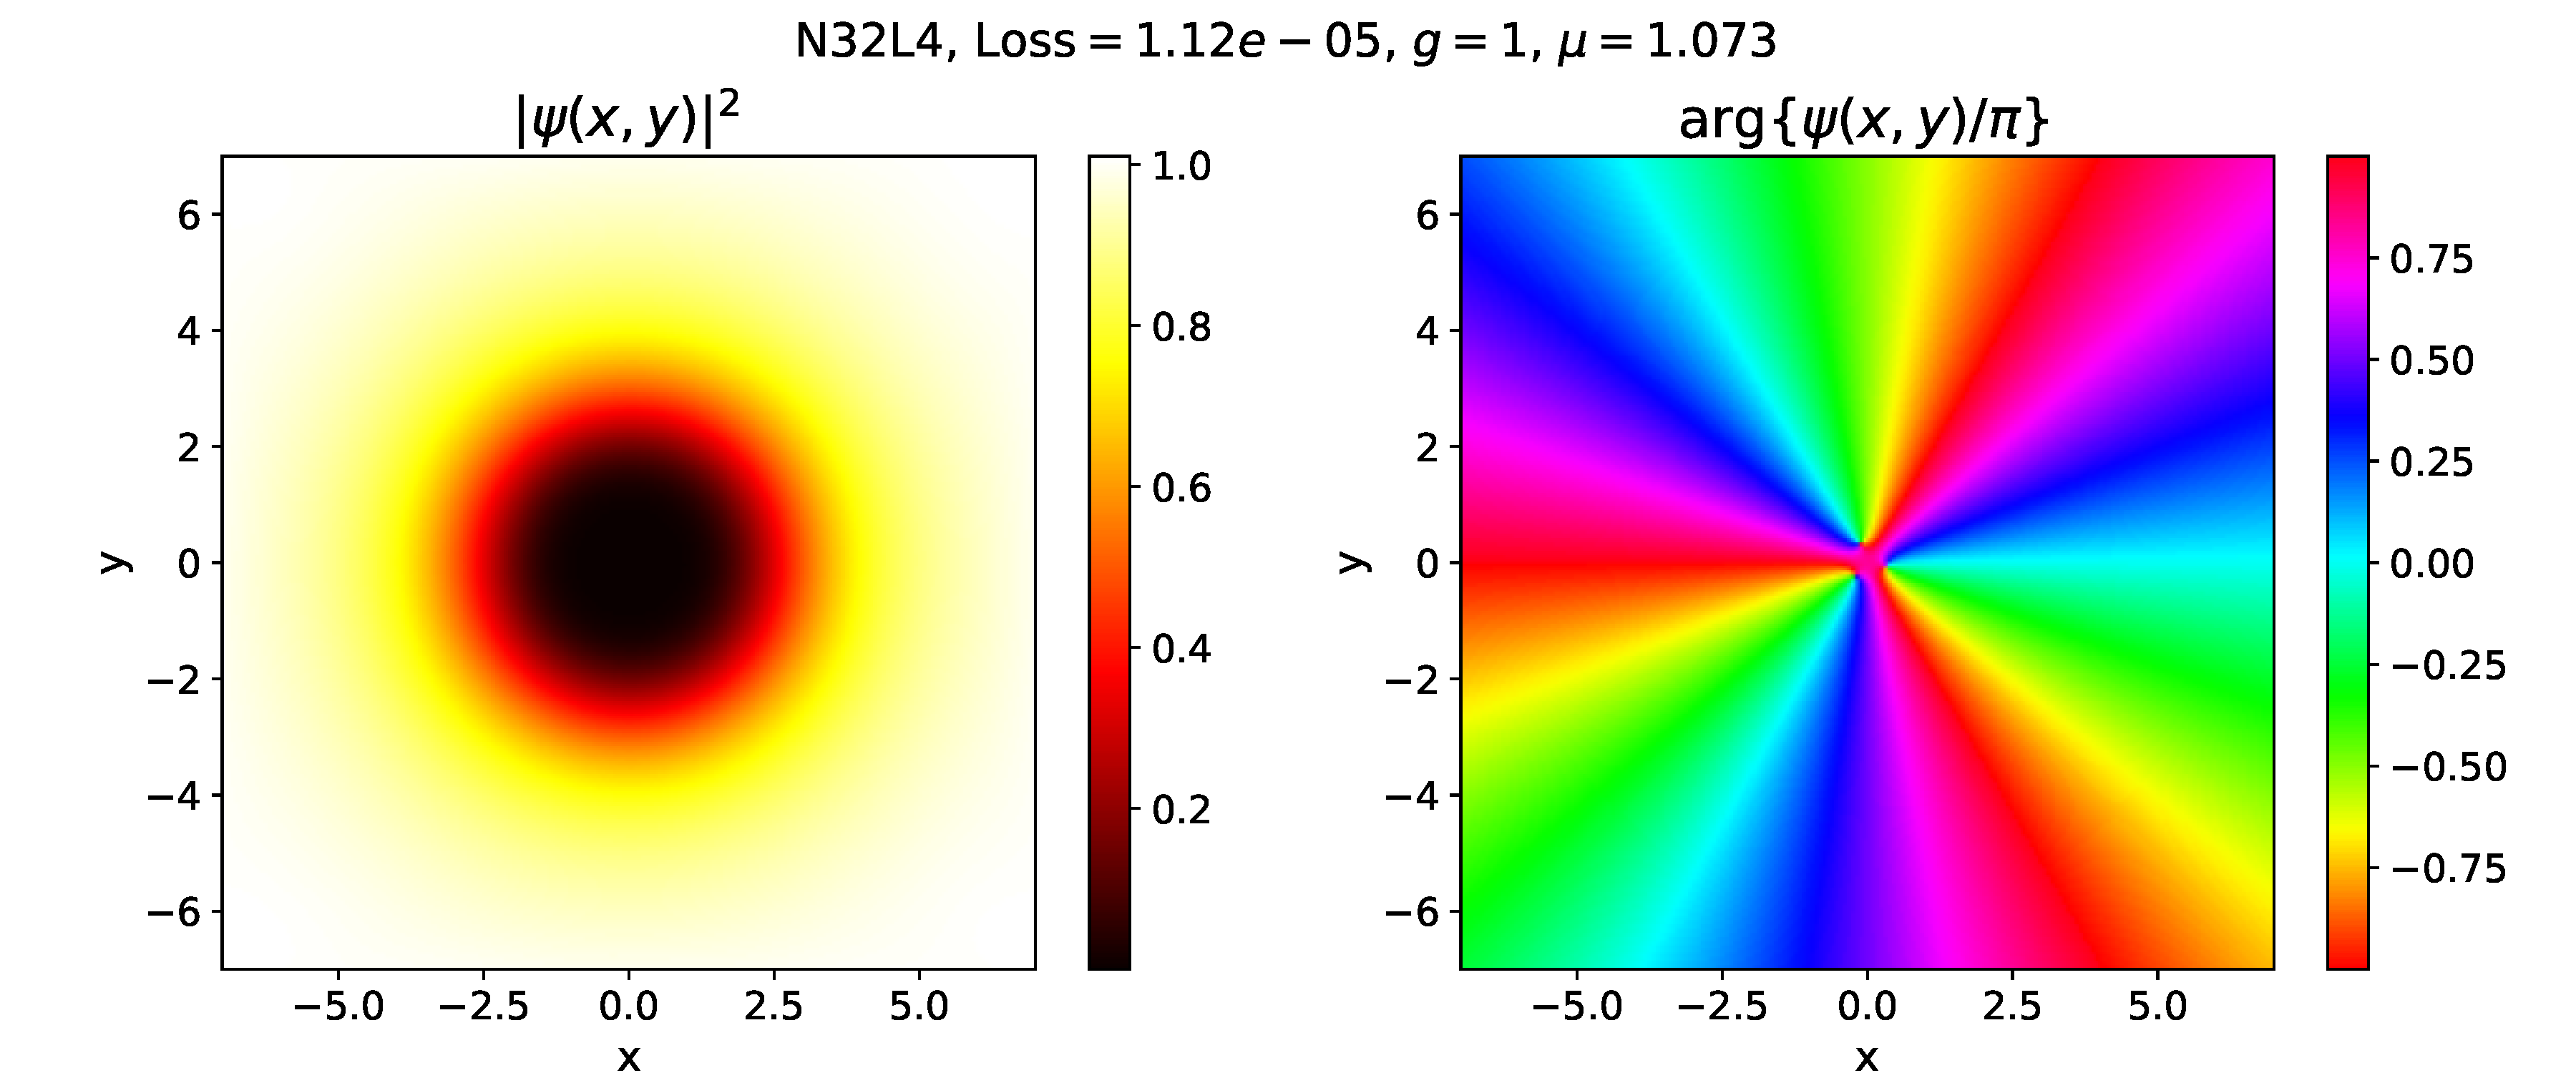
\includegraphics[width=\textwidth]{Figures/ex4_N32L4_PINN_Na1.0_x-7.00_-7.00-7.00_7.00_l3.png}
    \caption{Vortex solution of the 2D GPE with $g = 1$ and winding number 
    $m = 3$, the vortex is bigger than the one with $m = 1$.}
    \label{fig:vortex_l3}
\end{figure}
\begin{figure}[h!!!]
    \centering
    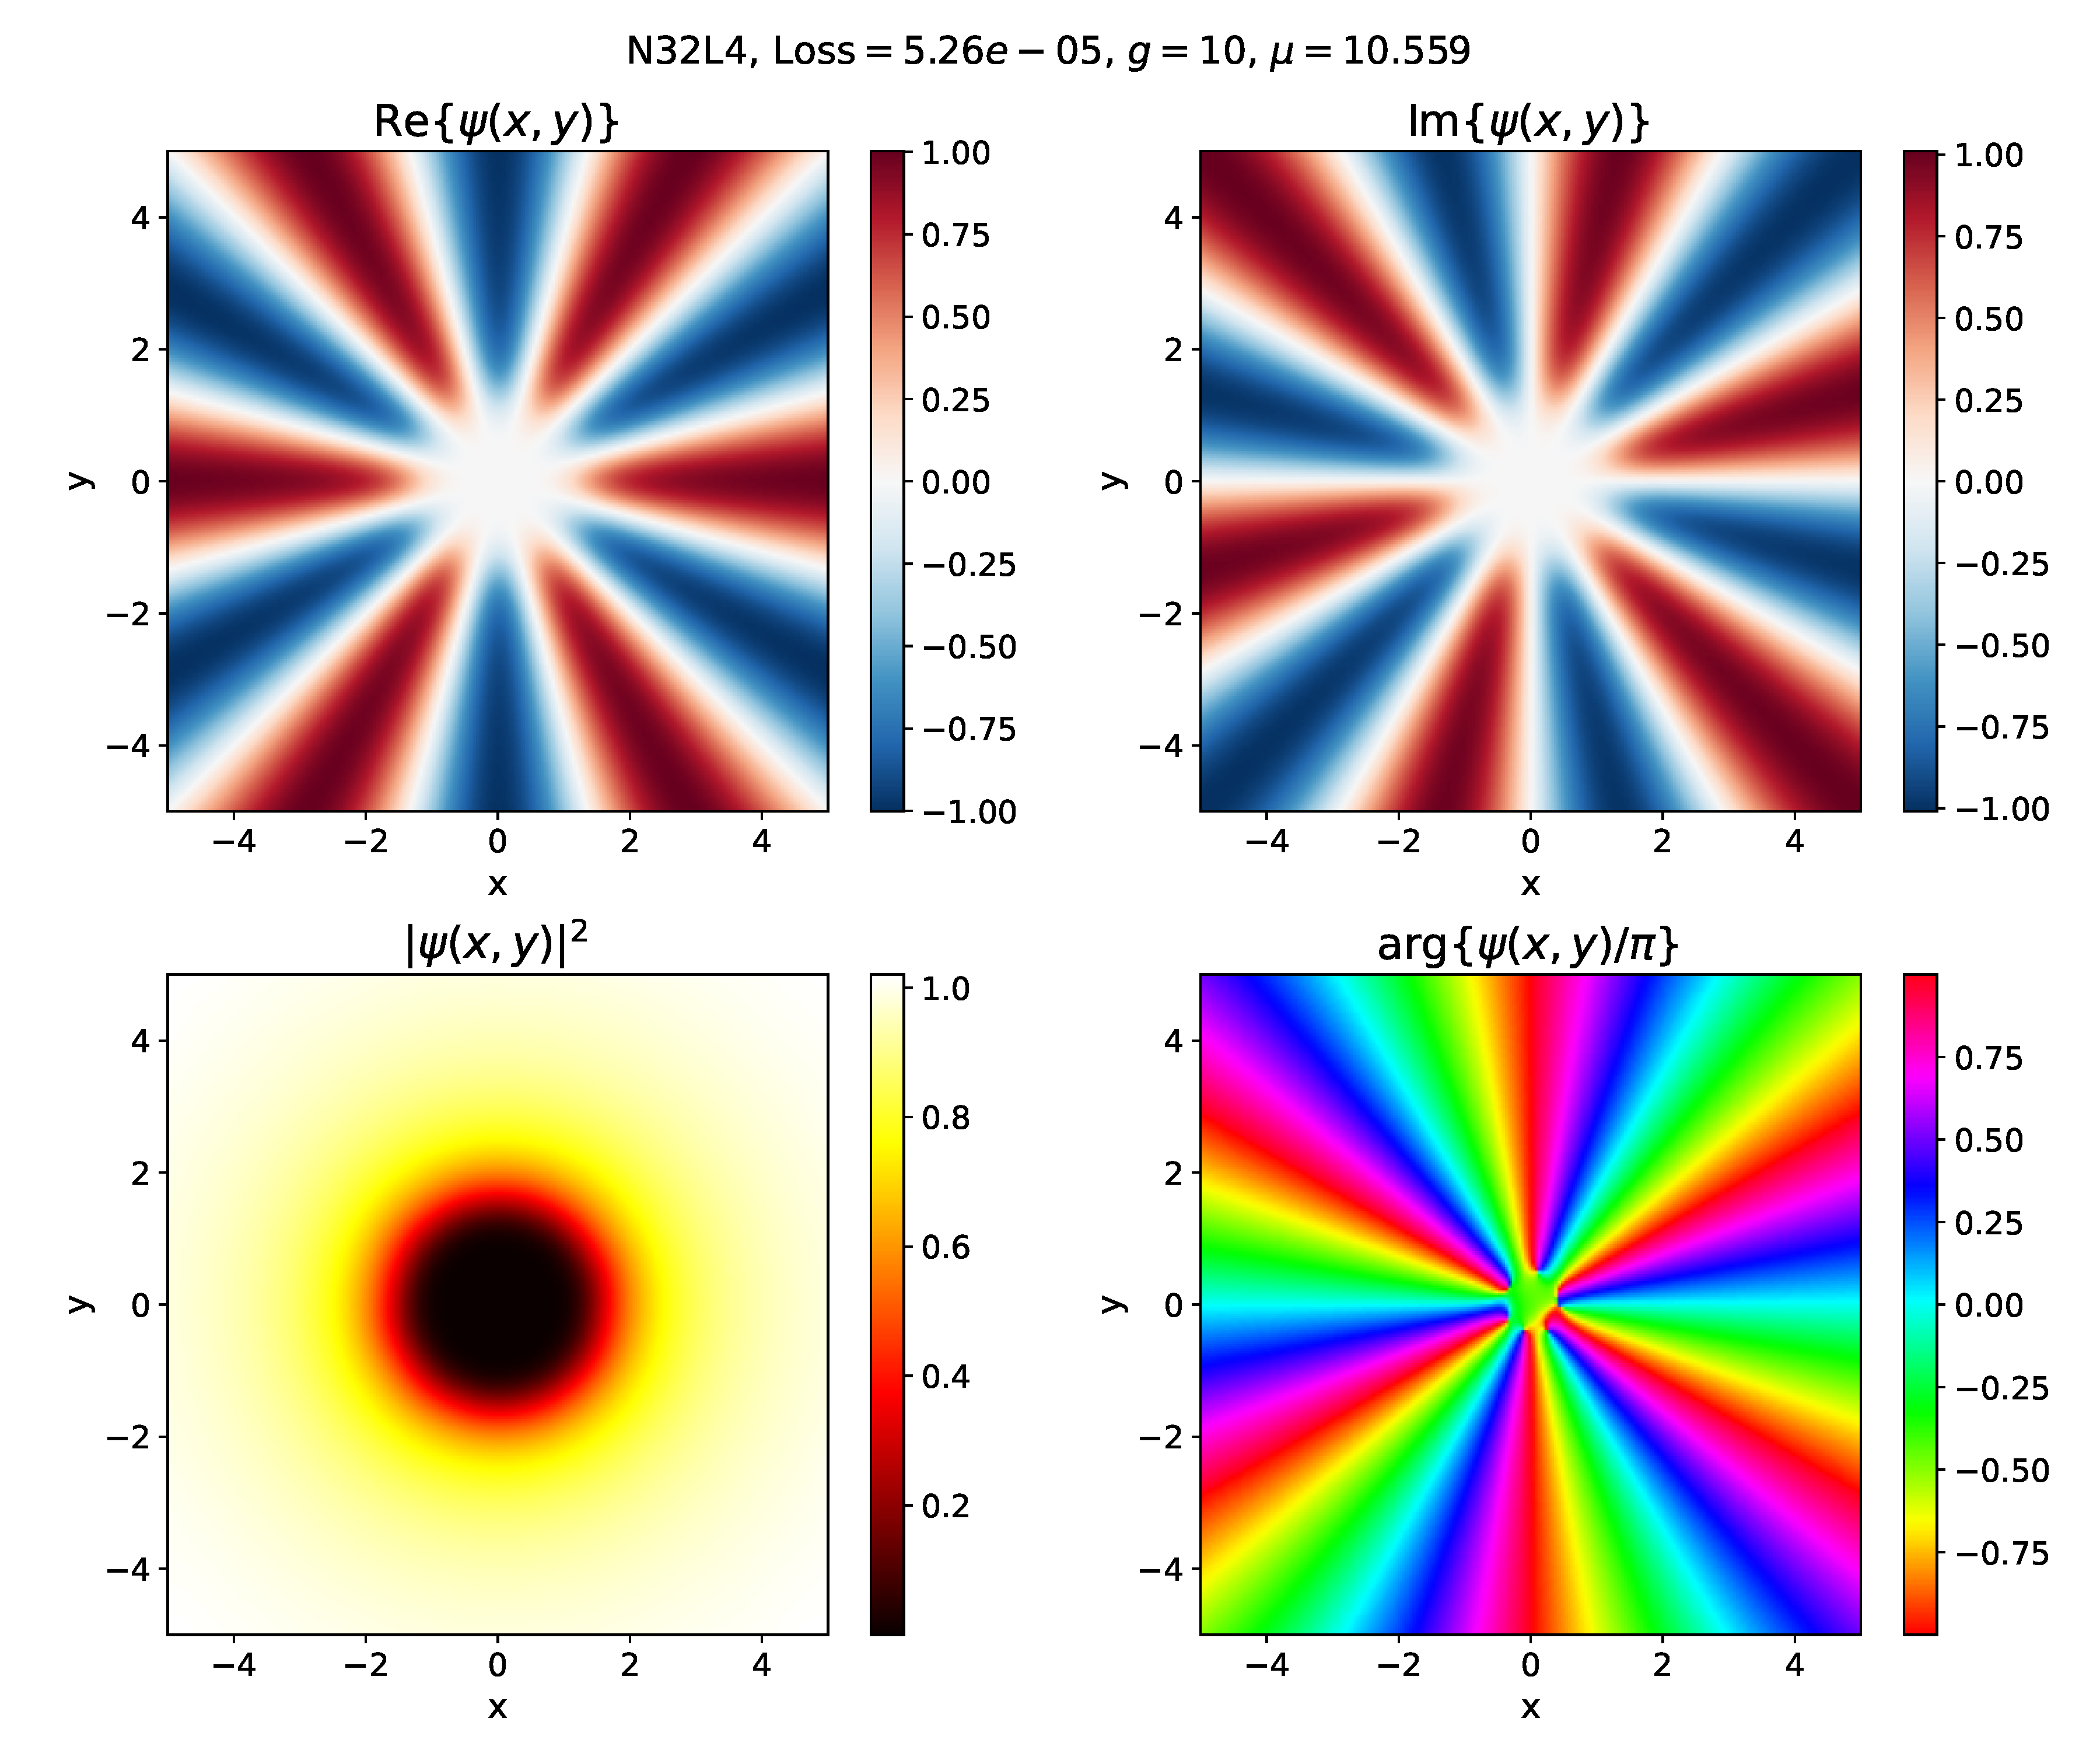
\includegraphics[width=\textwidth]{Figures/ex4_N32L4_PINN_Na10.0_x-5.00_-5.00-5.00_5.00_l6_full.png}
    \caption{Vortex solution of the 2D GPE with $g = 10$. When the interaction
    is stronger the vortex is smaller, allowing to find a solution with a 
    higher winding number $m = 6$ in a small domain.}
    \label{fig:vortex_l6}
\end{figure}




\section*{Conclusion}

In this report we have demonstrated the effectiveness of Physics-Informed Neural
Networks as a flexible and accurate tool for solving nonlinear quantum mechanical
problems governed by the Gross-Pitaevskii equation, in both one and two
spatial dimensions.

Starting from the 1D radial GPE with a harmonic potential, we showed that even
very compact architectures (as small as N4L1, with only 13 trainable parameters)
are capable of reproducing the ground state wave function with relative
$\mathbb{L}_2$ errors of order $10^{-4}$--$10^{-5}$.
Notably, the PINN approach proved particularly valuable for the strongly
interacting case $Na = 100$, where conventional methods showed convergence
issues, and the NN unambiguously confirmed the variational result.
Moving to the time-dependent nonlinear Schrödinger equation in 2D, we
reproduced the benchmark of Raissi et al.~\cite{RAISSI2019686} using a
significantly smaller network (N32L3 vs.\ N100L5), confirming that the
framework is competitive even with reduced computational resources.

The double well problems highlighted the main challenge of PINNs for eigenvalue
problems: the tendency to concentrate the wave function in a single well and
neglect the rest once the normalization constraint is satisfied.
We addressed this with a continuation strategy, initializing the training at
high interaction strength $g$ and progressively reducing it to the target value,
which proved effective not only in 1D and 2D double wells, but also for a more 
complex 2D trap like a modulated Mexican hat.
As a final application, by directly encoding the phase winding as a boundary
condition, the PINN spontaneously developed quantized vortex solutions with
winding numbers up to $m = 6$, correctly reproducing the expected dependence
of the core size on both $m$ and $g$.

Across all problems where independent, if not exact, data was available, a low
training loss consistently correlated with a low $\mathbb{L}_2$ error, 
validating it as a reliable quality metric.
The choice of architecture, sampling points and loss weights remains more of an
art than a science, yet once the right constraints are in place the network
converges to physically meaningful solutions, and in several cases proved more
robust than conventional approaches.
What makes PINNs particularly appealing is a certain \emph{naturalness} as a
computational tool for physics: the absence of a mesh, automatic
differentiation, and the ability to encode physical laws directly into the loss
function make the method feel closer to the physics than a finite-difference
discretisation, with the added practical advantage of being able to resume and
continue the training of an already converged network.


\newpage
\appendix

\section{The Eigenvalue Problem} \label{app:eigenvalue}

The results obtained in section \ref{sec:1d_double_well} looked solid, but we
might still be worried that the procedure of starting from a highly interacting
regime, increasing the nonlinearity of the PDE, might have found some
incorrect solutions.
Our NN could, for example, be in an excited metastable state.

In this section we present a method to study the spectrum of the system and
find eigenvalues and eigenfunctions of the GPE in a more self-consistent way.
The only caveat is that the spectral theorem we rely on is only valid for linear
operators and the GPE is nonlinear.

We start by considering that the eigenstates, solutions of a Schr\"{o}dinger
equation, are orthogonal to each other, so we can enforce this constraint when
training the NN.
In particular, we can rewrite the problem as
\begin{align}
    &-\frac{1}{2} \dv[2]{\psi_n(x)}{x} 
    + \left(V_{\rm ext}(x) + g |\psi_n(x)|^2 - \mu_n\right) \psi_n(x) = 0 \\
    &\int_{x_l}^{x_r} \psi_n(x) \psi_m(x) dx = 0, \quad n \neq m
\end{align}
and define a NN that takes $n$ as input too $\mathcal N(x, n)$, so that the
loss function becomes
\begin{align}
    \mathcal L &= \mathcal L_{\rm PDE} + \mathcal L_{\rm BC} 
        + 10 ~ \mathcal L_{\rm norm} + \mathcal L_{\rm ortho} \\
    \mathcal L_{\rm PDE} &= \frac{1}{N_{\rm s}N} \sum_{n=1}^{N_{\rm s}} \sum_{i=1}^N
        \left( -\frac{1}{2} \dv[2]{\psi_n(x_i)}{x} + \left(V_{\rm ext}(x_i)
        + g |\psi_n(x_i)|^2 - \mu_n\right) \psi_n(x_i) \right)^2 \\
    \mathcal L_{\rm BC} &= \frac{1}{N_{\rm s}} \sum_{n=1}^{N_{\rm s}}
    \frac{|\psi_n(x_l)|^2 + |\psi_n(x_r)|^2}{2} \\
    \mathcal L_{\rm norm} &= \frac{1}{N_{\rm s}} \sum_{n=1}^{N_{\rm s}}
        \left( \frac{x_r - x_l}{N} \sum_{i = 1}^N \psi_n(x_i)^2  - 1 \right)^2 \\
    \mathcal L_{\rm ortho} &= \sum_{n \neq m} \left(\frac{x_r-x_l}{N}
        \sum_{i=1}^N \psi_n(x_i) \psi_m(x_i) \right)^2 \, .
\end{align}

We can now train the NN on a grid of $x \in [x_l, x_r]$ and 
$n \in [0, ~ 1, ~ ..., ~ N_{\rm s} - 1]$ where each n corresponds to a different
eigenstate and orthogonality is enforced between all the states.
Of course, we have no guarantee that the NN will learn the states in the correct 
order, nor that it will learn the lowest energy ones, but if we choose
$N_{\rm s} = 6$ we still have a good chance of finding the ground state.

Figure \ref{fig:ex3.5_harmonic_eigen} shows the results for the harmonic
potential with $g = 0$, of which the spectrum is known analytically to be
$\mu = \frac{1}{2} + \tilde n, ~ \tilde n = 0, 1, ...$, and we can
see that the NN correctly learns the 6 eigenstates of the system (that we 
ordered from the one with the lowest $\mu$ to the one with the highest $\mu$),
but happened to miss the 5th one.

Figures \ref{fig:ex3.5_dw2_eigen} and \ref{fig:ex3.5_dw1_as6_eigen} show instead
the results for the symmetric and non-symmetric double well potentials used in 
section \ref{sec:1d_double_well} (Figures \ref{fig:ex3_dw2_yee_g1} and 
\ref{fig:ex3_dw1_as6} respectively).

This method is not intended to find the entire spectrum of the system, nor to 
accurately predict the wave functions, but it has a high chance of finding the
ground state immediately and in a self-consistent way, considering that every
state found must be orthogonal to the others.
We can also use the results to get an idea of the spectrum of the system and
use this information to guide the optimizer in the early stages of the training
that was done in section \ref{sec:1d_double_well}.

A more precise assessment of the precision of the ground state found with this
method is presented in Figure \ref{fig:ex3.5_dw2_check} and Figure
\ref{fig:ex3.5_dw1_as6_check}, where we compare the results obtained with the
two different methods.
A non-perfect agreement is to be expected considering that when computing more
eigenstates the optimizer only reached a loss of $\sim 10^{-4}$, while in the 
previous section we were able to reach a loss of $\sim 10^{-6}$.
For the double well potential with $a = 2$ the relative $\mathbb L_2$ error is
$9.92 \times 10^{-3}$, while for the non-symmetric double well potential it is
$4.43 \times 10^{-3}$.
Part of the error could also be due to the fact that imposing the orthogonality
constraint would only be justified when $g = 0$ (when the GPE reduces to a 
linear Schr\"{o}dinger equation), while in this case we have $g = 1$.
Indeed, even at $g=0$ it can be a starting point to find the solution of the
interacting problem.

\begin{figure}[]
    \centering
    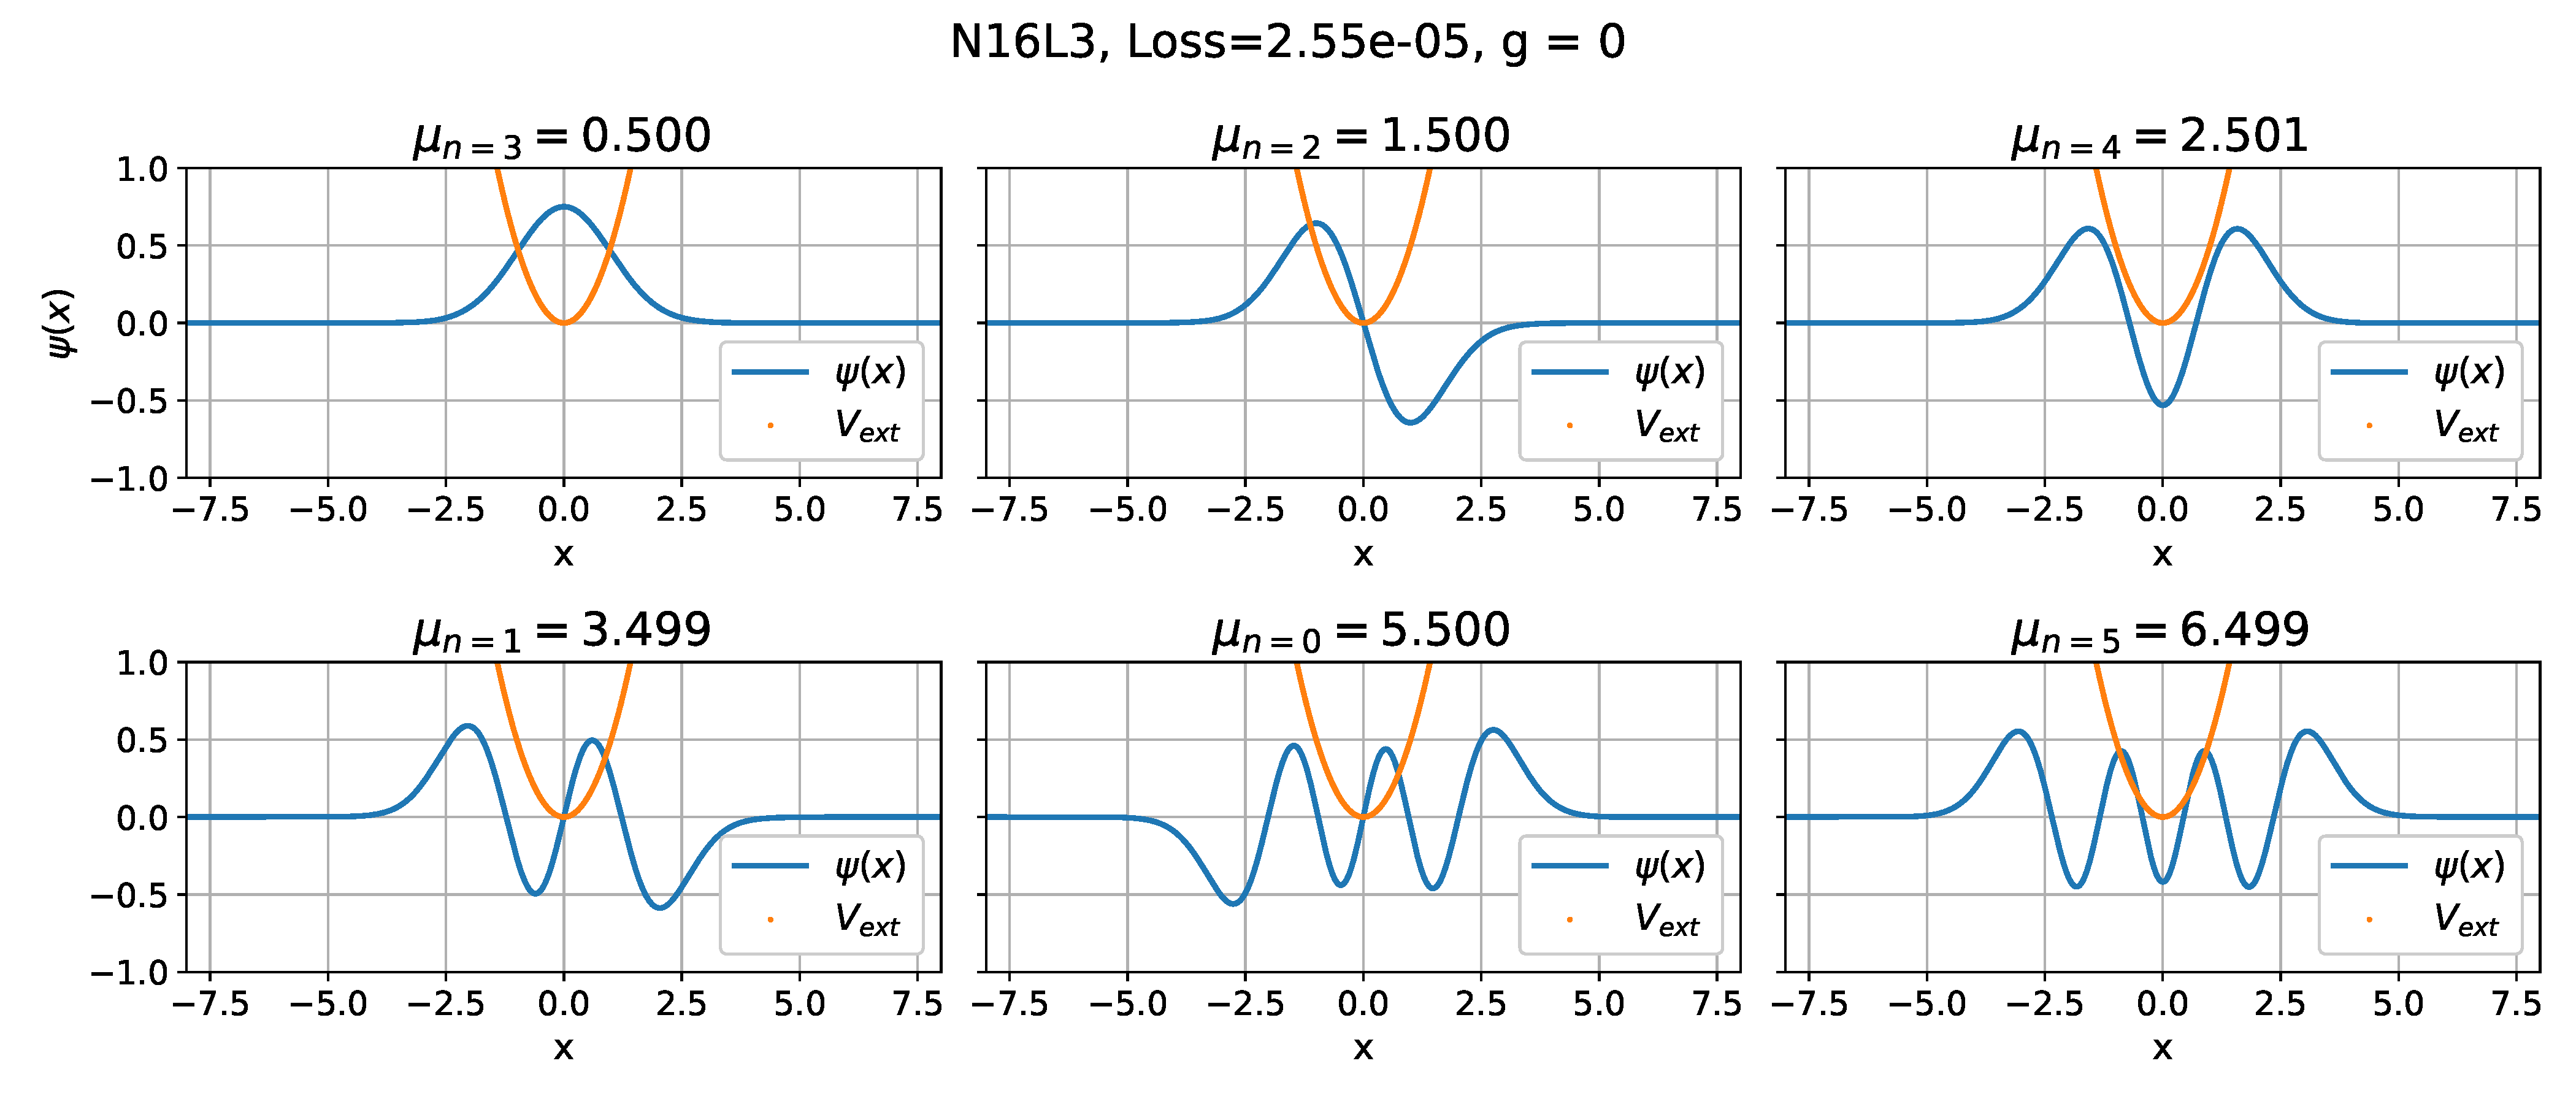
\includegraphics[width=\textwidth]{Figures/ex3.5_N16L3_PINN_Na0.0_x-8.00-8.00_harmonic_eigen.png}
    \caption{1D GPE with $g = 0$ and a harmonic potential.
    The same NN correctly learns 6 eigenstates (that in this case are known
    analytically) but misses the 5th one.}
    \label{fig:ex3.5_harmonic_eigen}
\end{figure}
\begin{figure}[]
    \centering
    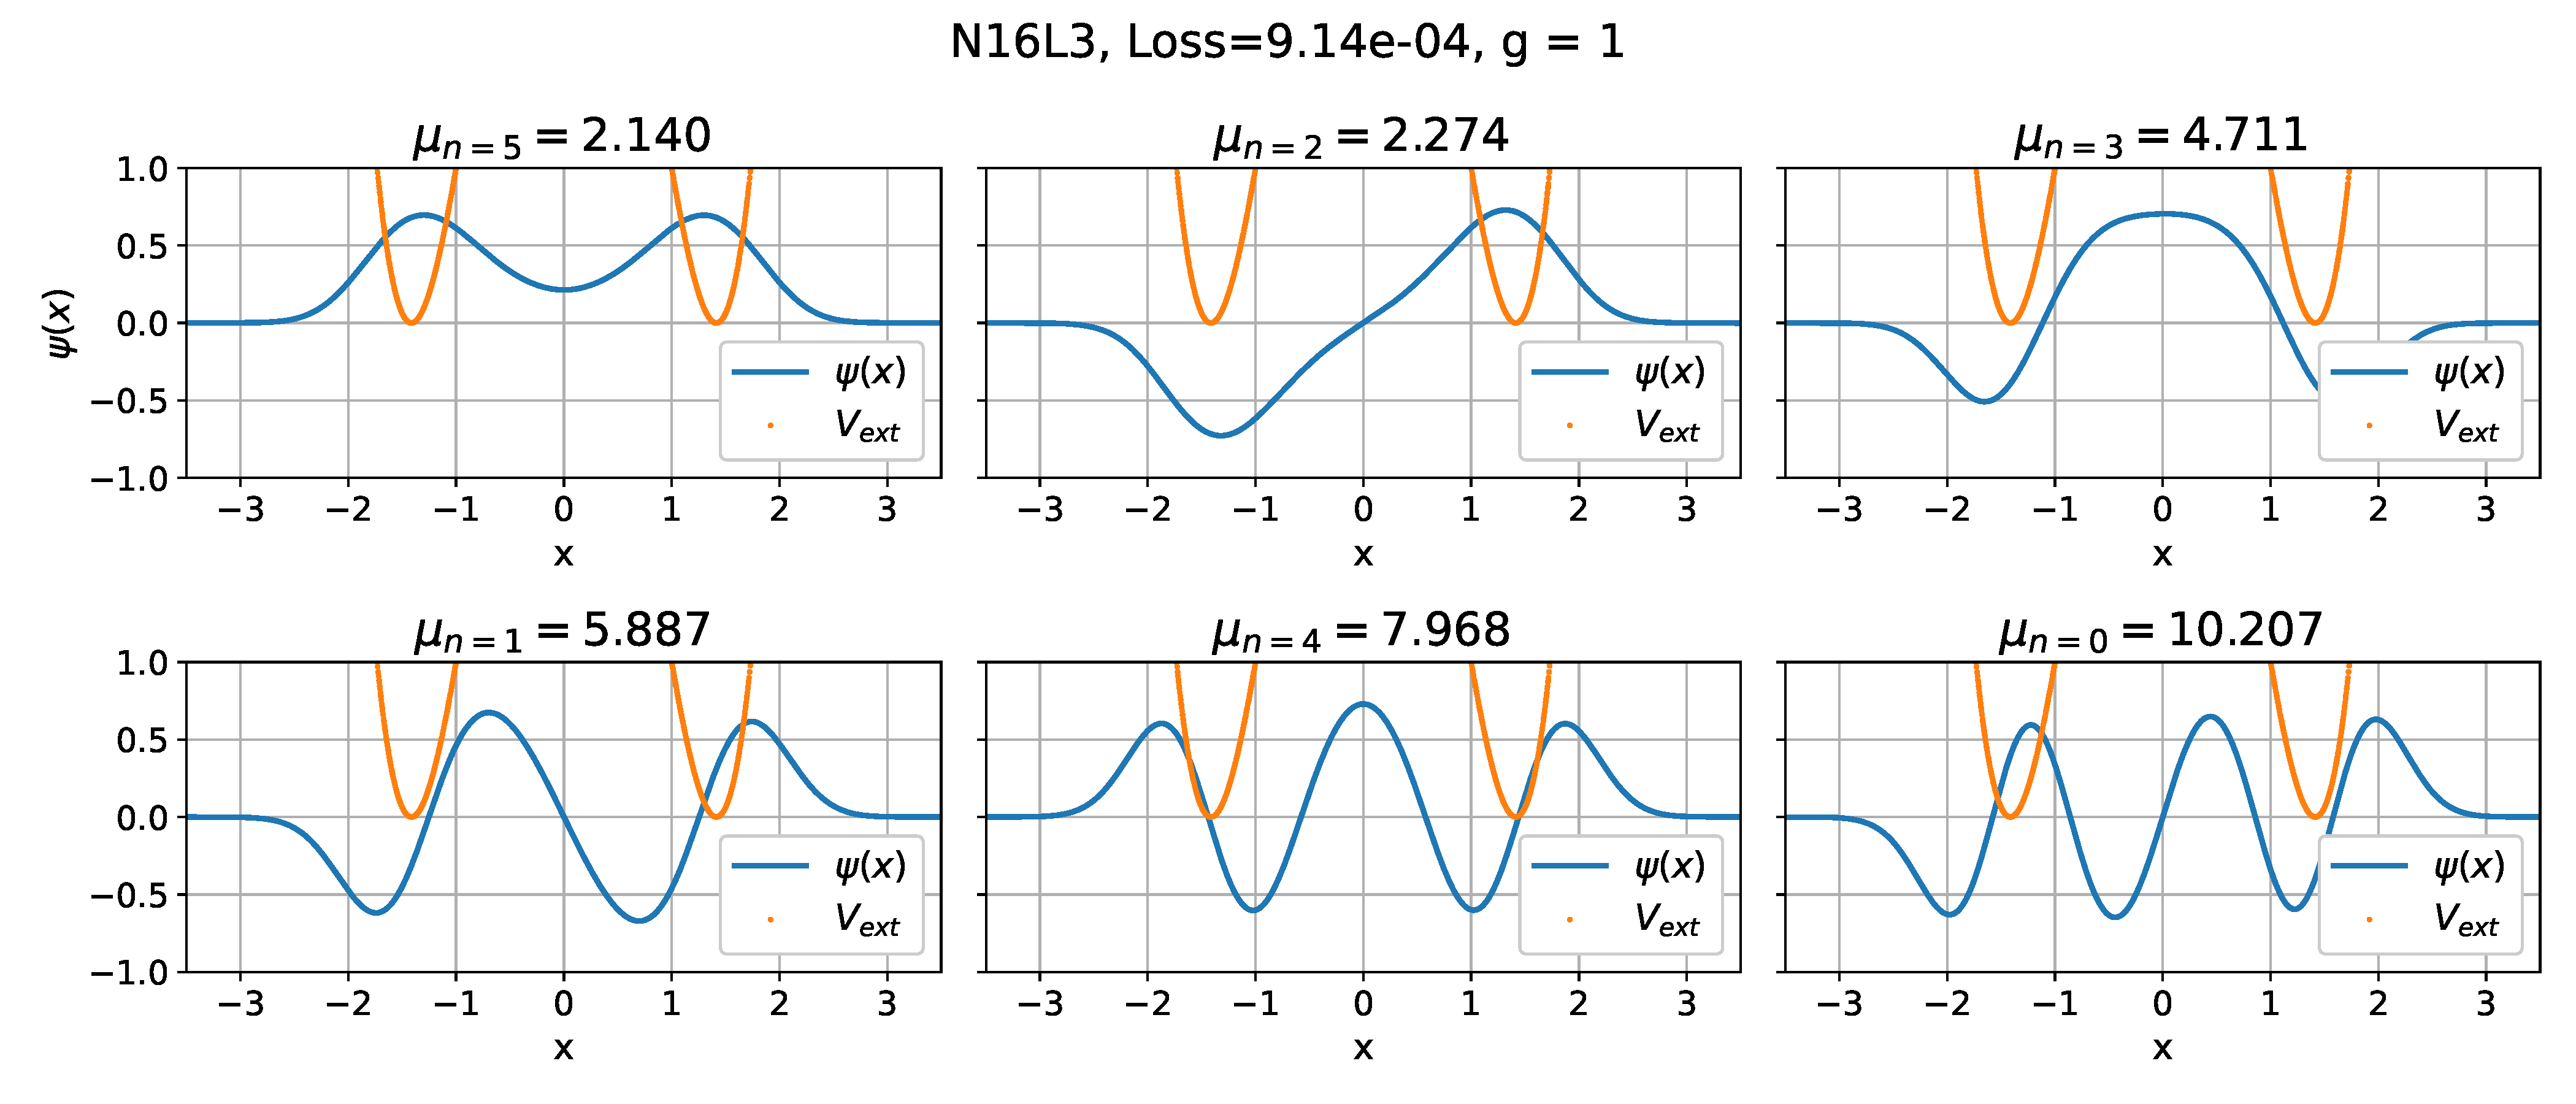
\includegraphics[width=\textwidth]{Figures/ex3.5_N16L3_PINN_Na1.0_x-3.50-3.50_dw2_eigen.png}
    \caption{Results for the 1D GPE with $g = 1$ and a symmetric double well
    potential from equation \eqref{eq:dw} with $a = 2$ using a NN with N16L3.}
    \label{fig:ex3.5_dw2_eigen}
\end{figure}
\begin{figure}[]
    \centering
    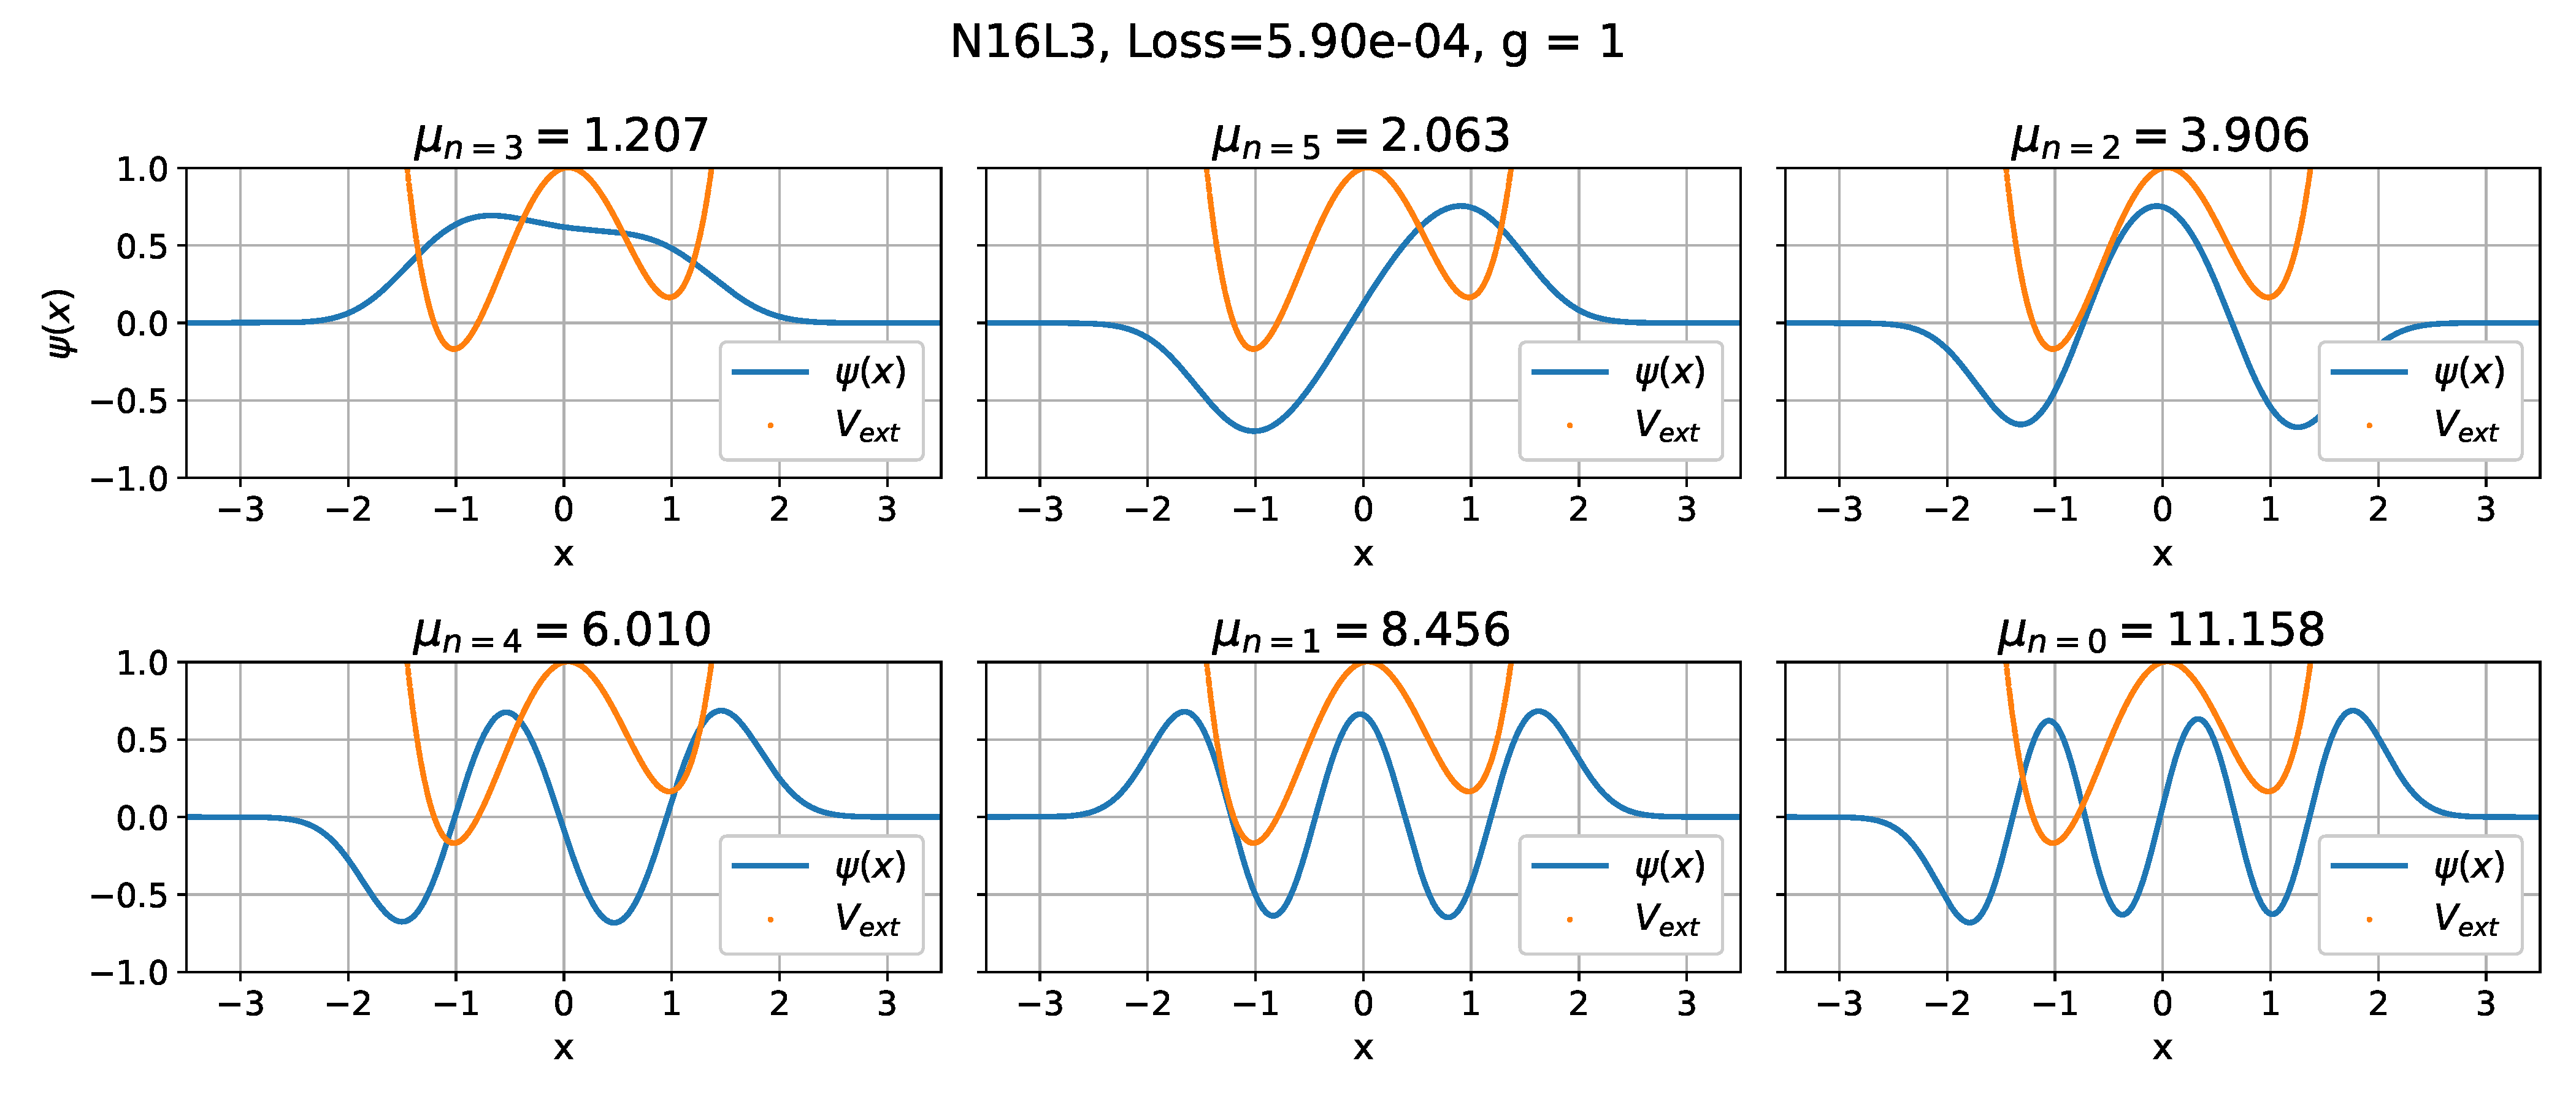
\includegraphics[width=\textwidth]{Figures/ex3.5_N16L3_PINN_Na1.0_x-3.50-3.50_dw1_as6_eigen.png}
    \caption{Results for the 1D GPE with $g = 1$ and a non-symmetric double well
    potential from equation \eqref{eq:dw_as} with $a = 1$ and $b = 6$ using a NN 
    with N16L3.}
    \label{fig:ex3.5_dw1_as6_eigen}
\end{figure}


\begin{figure}[h!]
\begin{minipage}{0.48\textwidth}
    \centering
    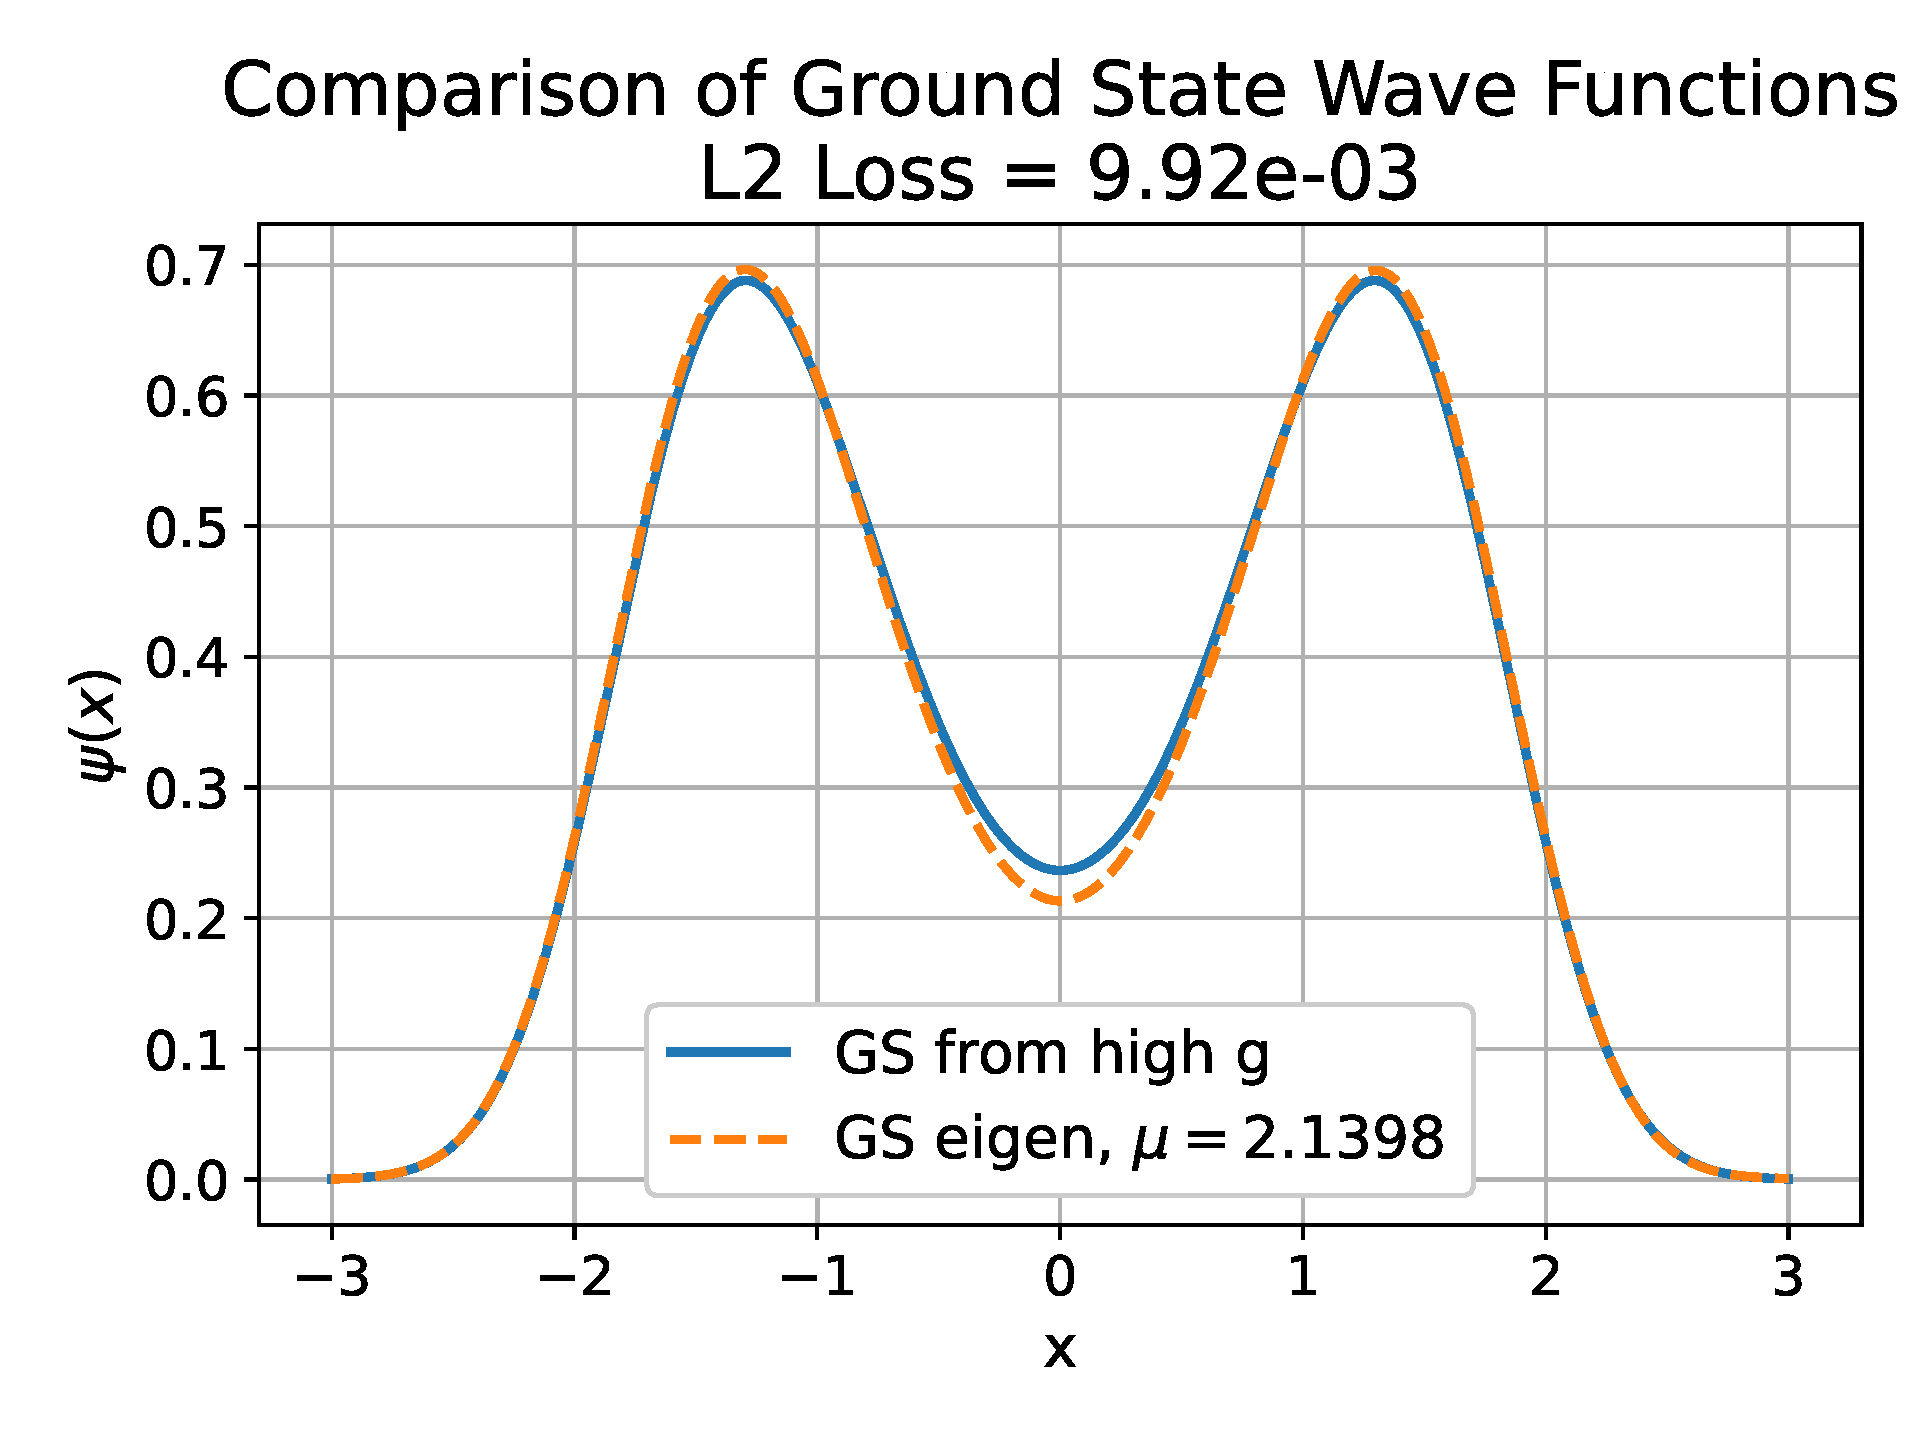
\includegraphics[width=\textwidth]{Figures/ex3.5_1D_dw2_high_g_comparison.png}
    \caption{Comparison of the results obtained for the double well potential
    with $a = 2$ and $g = 1$ with the method of section \ref{sec:1d_double_well}
    (solid blue line) and the method of Appendix \ref{app:eigenvalue}
    (orange dotted line).}
    \label{fig:ex3.5_dw2_check}
\end{minipage}
\hspace{0.05\textwidth}
\begin{minipage}{0.48\textwidth}
    \centering
    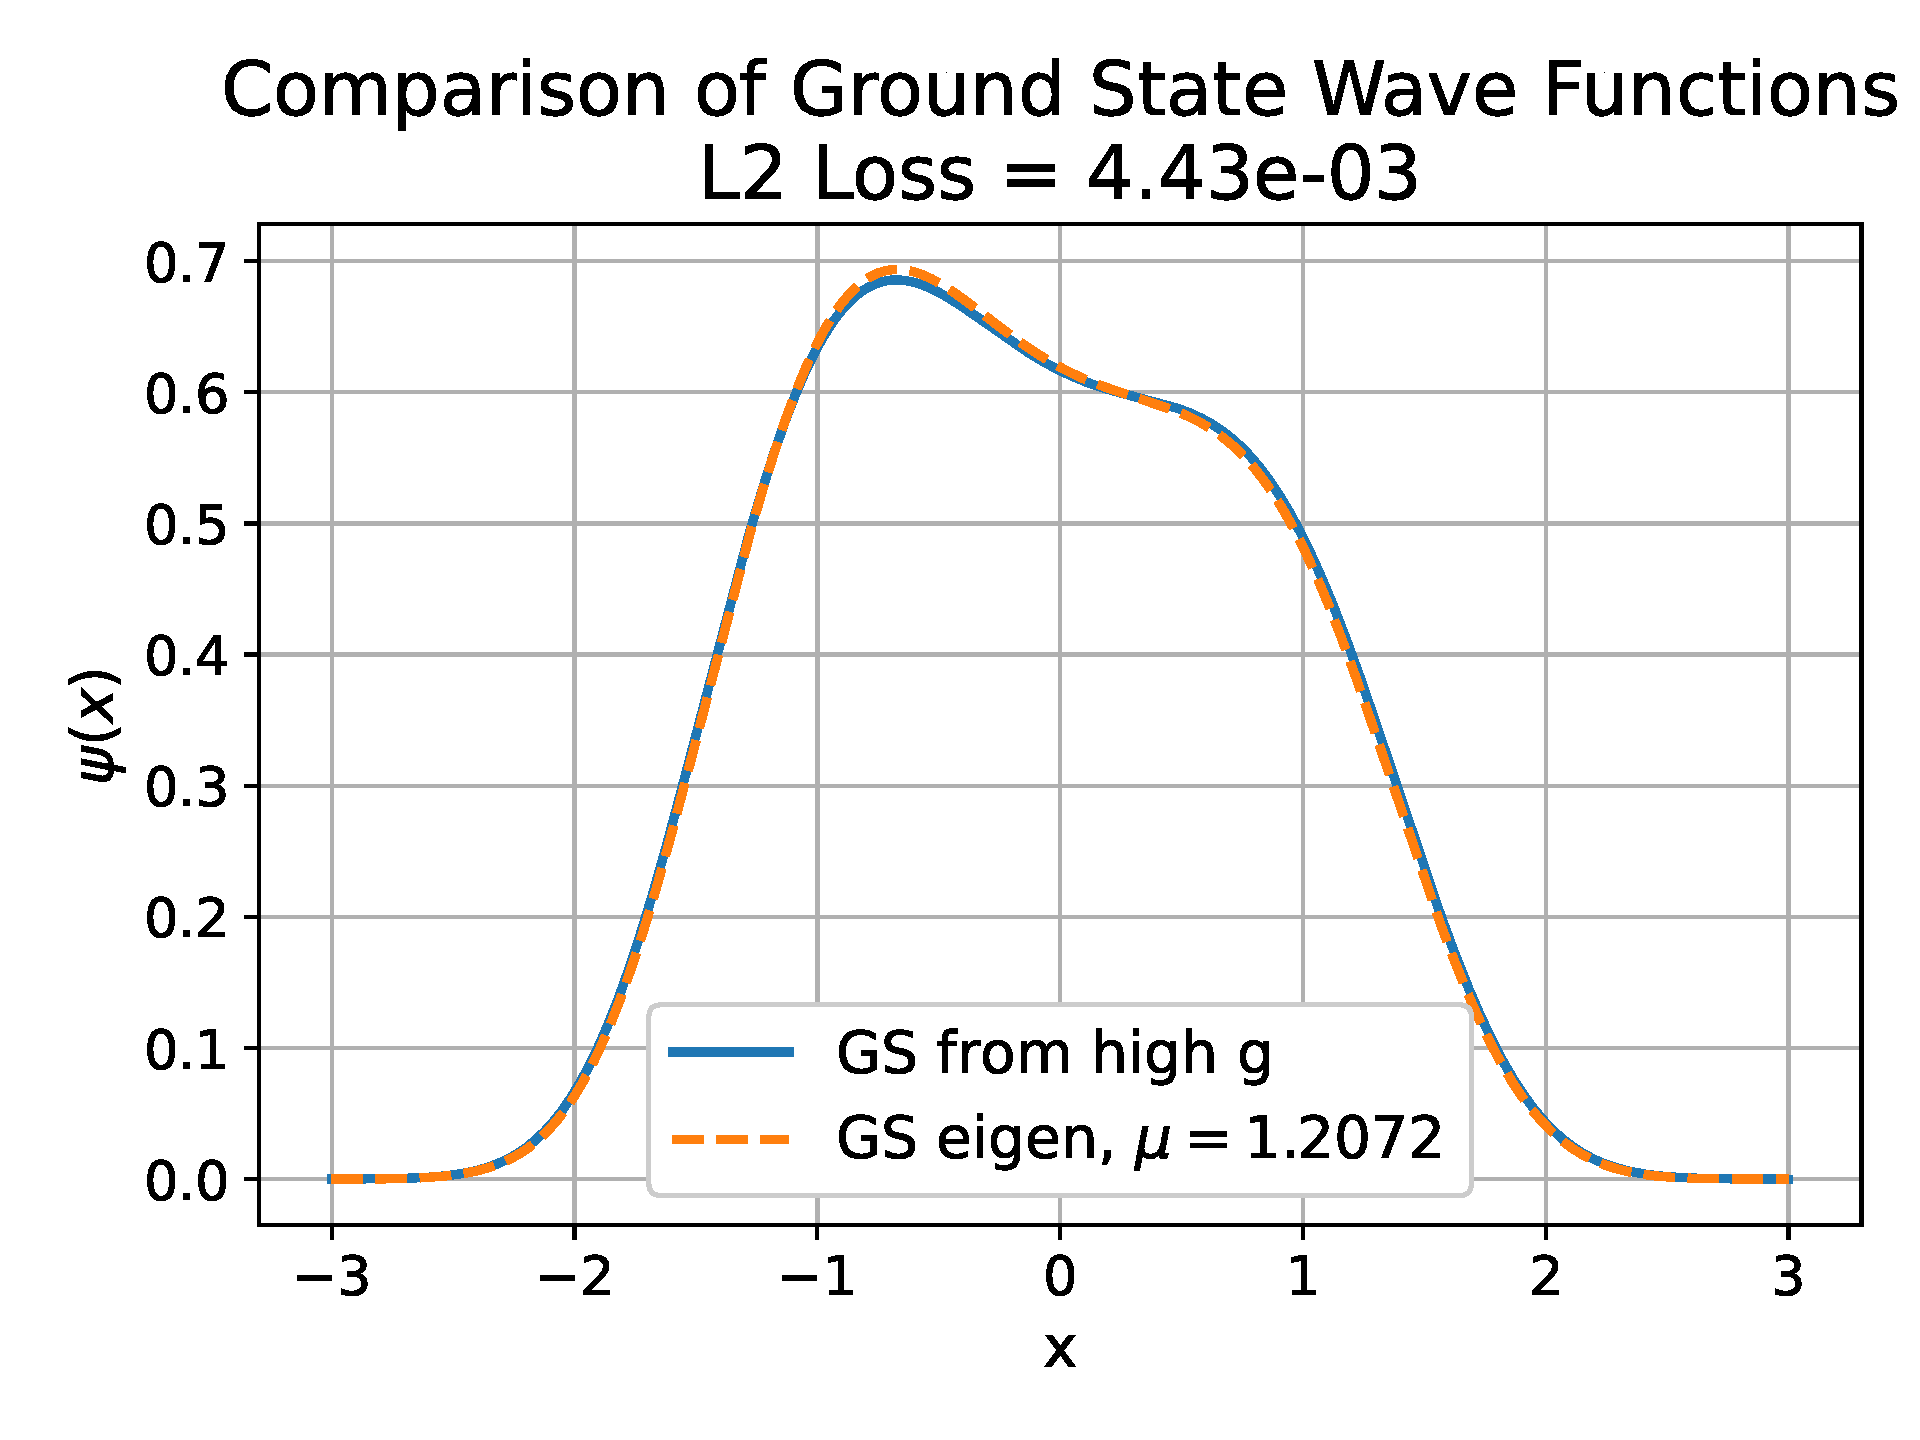
\includegraphics[width=\textwidth]{Figures/ex3.5_1D_dw1_as6_high_g_comparison.png}
    \caption{Comparison of the results obtained for the non-symmetric double well
    potential with $a = 1$, $b = 6$ and $g = 1$ with the method of section
    \ref{sec:1d_double_well} (solid blue line) and the method of Appendix
    \ref{app:eigenvalue} (orange dotted line).}
    \label{fig:ex3.5_dw1_as6_check}
\end{minipage}
\end{figure}


Extending this method to 2D for a harmonic potential we correctly recover 
the ground states and the excited eigenstates with non-zero angular momentum,
as shown in Figure \ref{fig:ex3.5_2D_harmonic_eigen}.
\begin{figure}[h!!!]
    \centering
    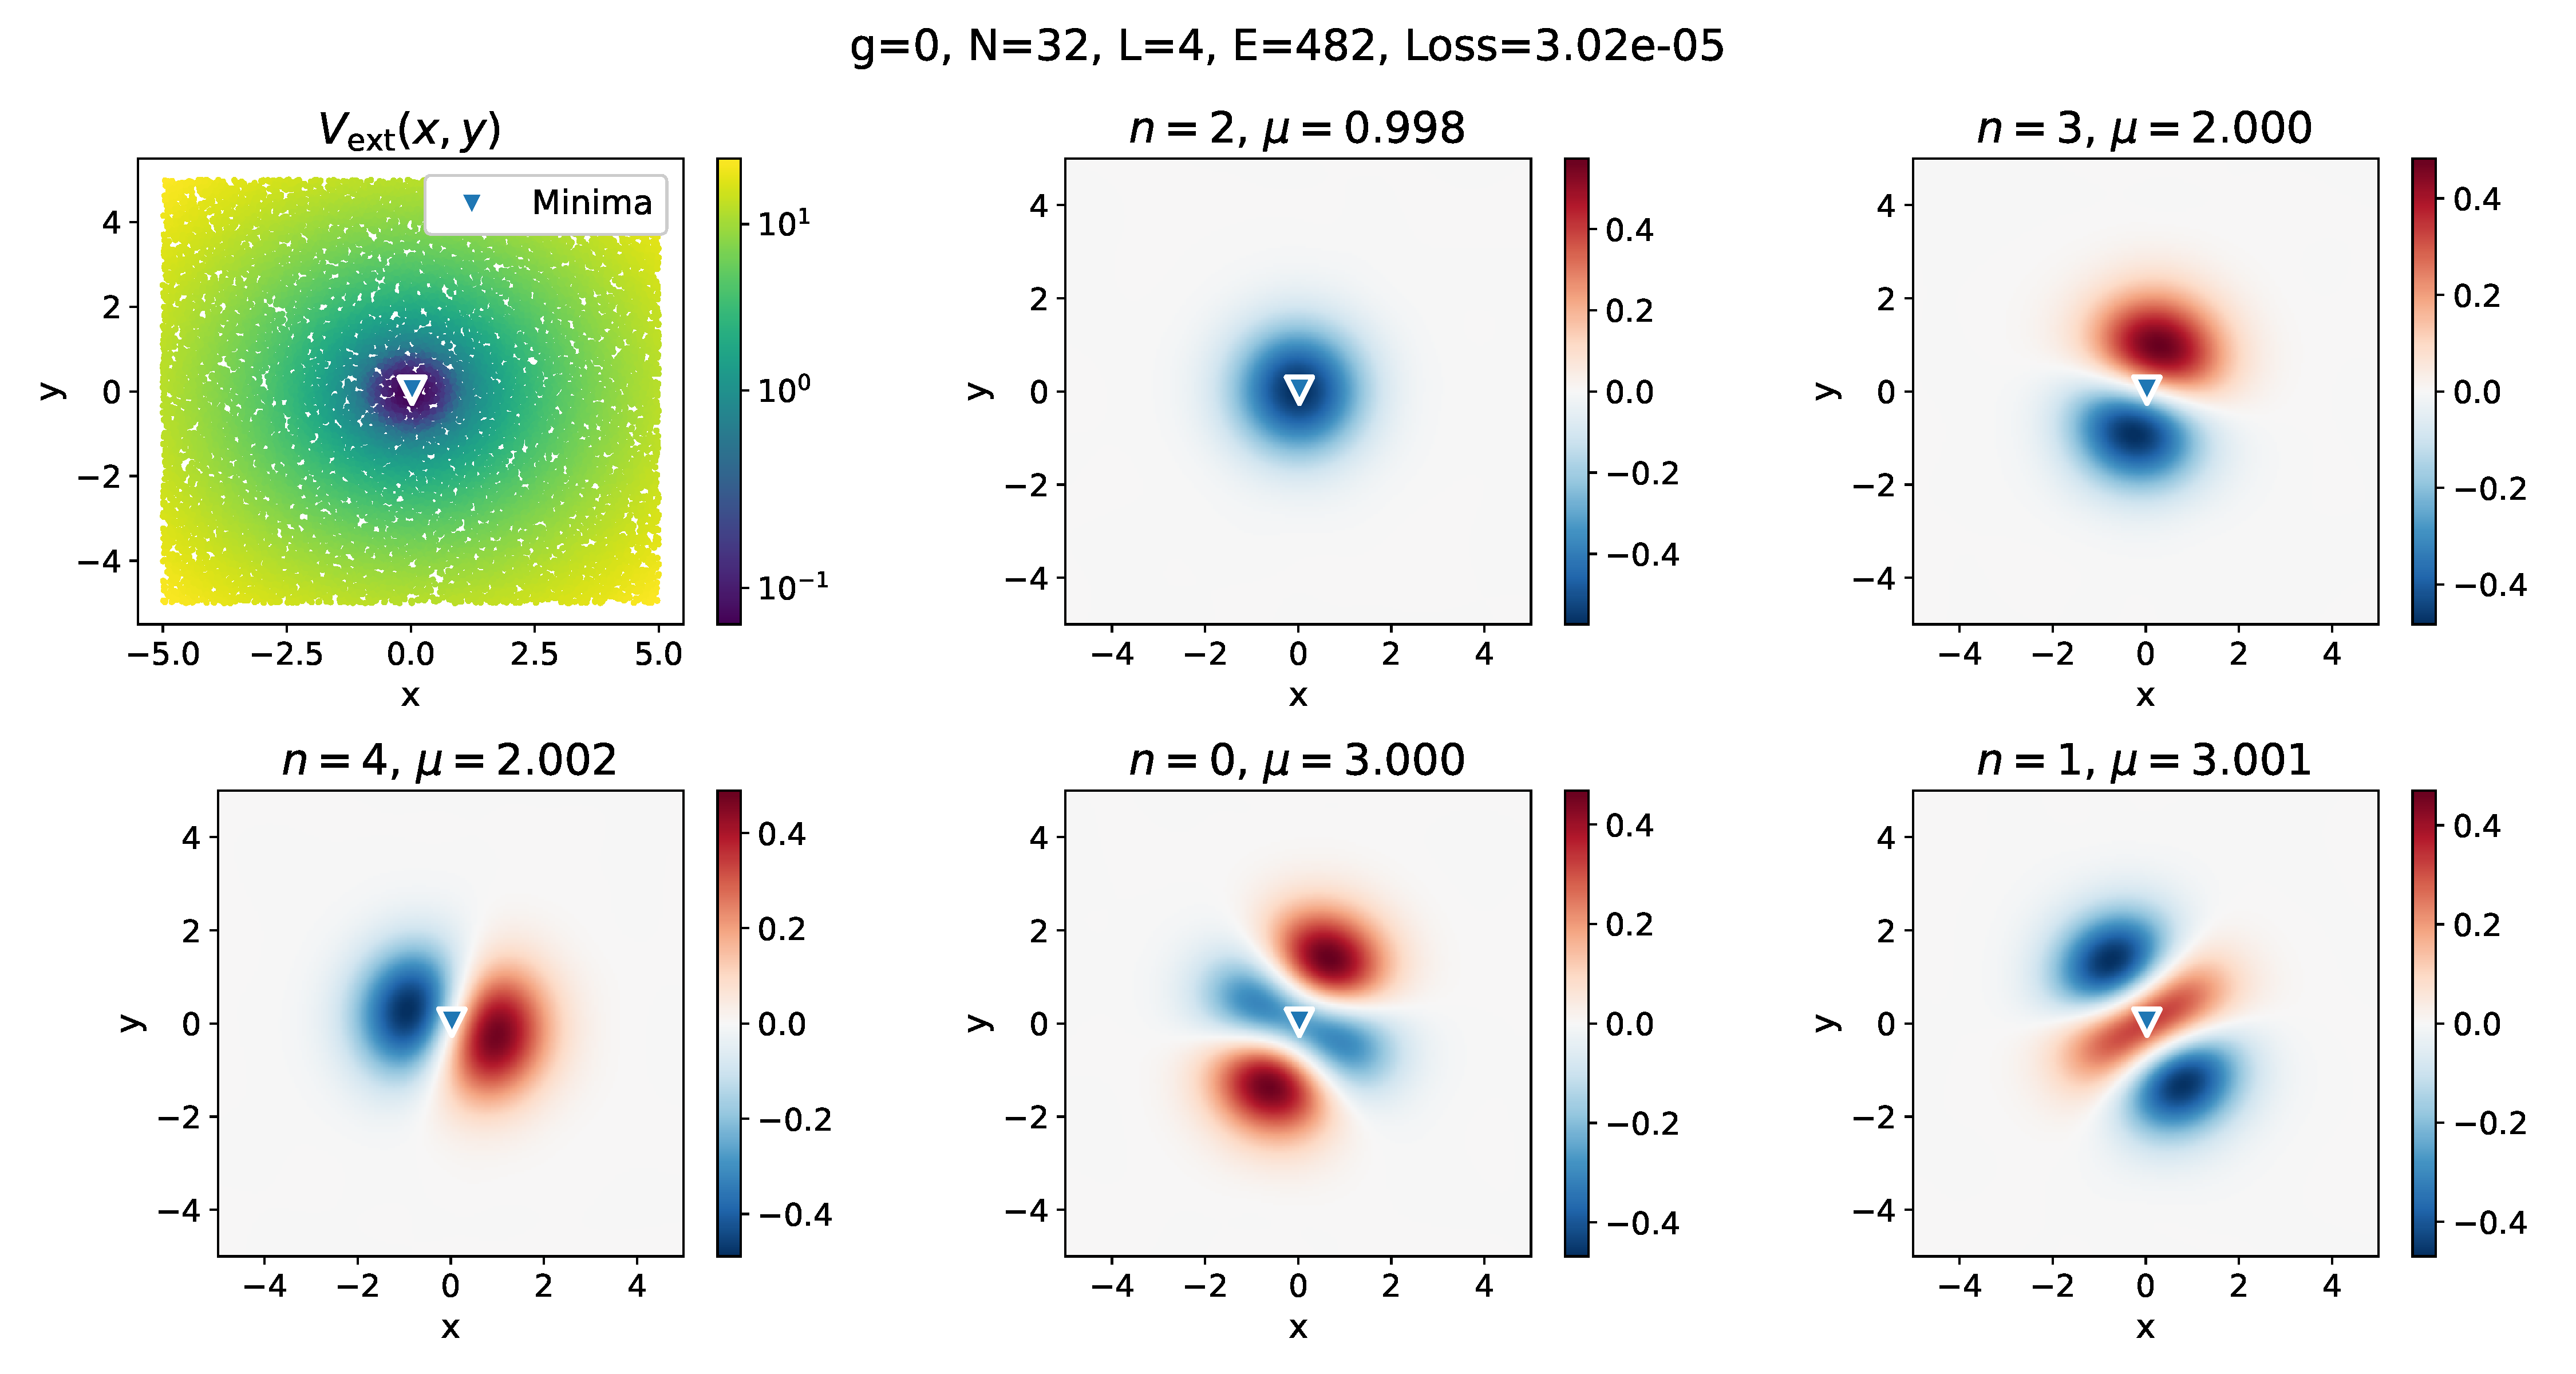
\includegraphics[width=\textwidth]
    {Figures/ex3.5_N32L4_PINN_Na0.0_x-5.00_-5.00-5.00_5.00_harmonic_eigen.png}
    \caption{Five eigenstates of the 2D GPE with $g = 1$ and a harmonic
    potential, computed with a N32L4 NN.
    The ground state ($n = 3$) and two pairs of degenerate excited states are
    found, with the degeneracy consistent with the rotational symmetry of the
    harmonic potential.}
    \label{fig:ex3.5_2D_harmonic_eigen}
\end{figure}

For a double well however, the method fails, as the NN consistently converges
to an excited state with the probability localized in a single well and never
to the ground one.




\newpage
\section{Spread-Out Potential} \label{app:spread_out_potential}

In the section \ref{sec:1d_double_well}, we developed a strategy to force the
wave function to spread over the entire domain by increasing the interaction
strength $g$. 
Later we observed that this method worked well in 2D (Section 
\ref{sec:2d_double_well}) and with a more complex potential (Section 
\ref{sec:complex_2d_traps}).

As a further test, we present here an even more complex potential to test the
ability of the PINN to spread the wave function over multiple wells distributed 
across the domain.
\begin{equation}
    V_{\rm ext}(x,y) = \frac{1}{2}\,\omega (x^2 + y^2)
    + V_0 \sum_{k=0}^4 \cos\left(2\pi\left(x\cos\theta_k + y\sin\theta_k\right)\right),
    \qquad
    \theta_k = \frac{2\pi k}{5}\,,
    \label{eq:spread_out_potential}
\end{equation}
is a superposition of a harmonic trap and a five-fold angular modulation
that creates a pattern of small potential wells, a representation of which is
shown in the left panel of Figure \ref{fig:ex3_quasicrystal_g1000}.

We use $\omega = 0.1$ and $V_0 = 1$, so that the potential is not dominated by
the harmonic term and the wave function is expected to spread more over the
entire domain (while still being confident by the harmonic trap).
For this reason, we also drop the boundary condition requiring the wave
function to vanish at the boundary. The loss therefore consists only of the PDE
term $\mathcal{L}_{\rm PDE}$ and the normalization term
$\mathcal{L}_{\rm norm}$.

Figure~\ref{fig:ex3_quasicrystal_g1000} shows the potential alongside the
solution obtained with an N32L3 neural network for $g = 1000$. We use 40,000
sample points to compute $\mathcal{L}_{\rm PDE}$ and
$\mathcal{L}_{\rm norm}$. Inspecting the potential (left panel of
Figure~\ref{fig:ex3_quasicrystal_g1000}) we observe an inner ring with a
minimum of $-1.94$, a ring of small wells with a common minimum of $-3.11$,
and an outer ring of even smaller wells with a common minimum of $-1.56$.

We then proceed by reducing $g$ by $10\%$ at each step and retraining the
network down to $g = 1$, each time reaching \texttt{L-BFGS} convergence with a
loss below $10^{-4}$.
Two intermediate solutions are shown in Figure
\ref{fig:ex3_quasicrystal_intermediate} to appreciate how the wave function 
becomes progressively more localized, but still keeping the pattern of the
potential in the outer ring of wells.
Finally, the solution for $g = 1$ is shown in Figure
\ref{fig:ex3_quasicrystal_g1}, where we can see that the wave function is
mostly localized in the inner ring and in the middle ring, even though the wells 
in the middle ring are deeper. On the right panel of Figure 
\ref{fig:ex3_quasicrystal_g1} we stretch the color scale to better visualize 
that the effect of the outer ring is still somewhat visible, even though the 
wave function is very small in that region.

\begin{figure}[ht]
    \centering
    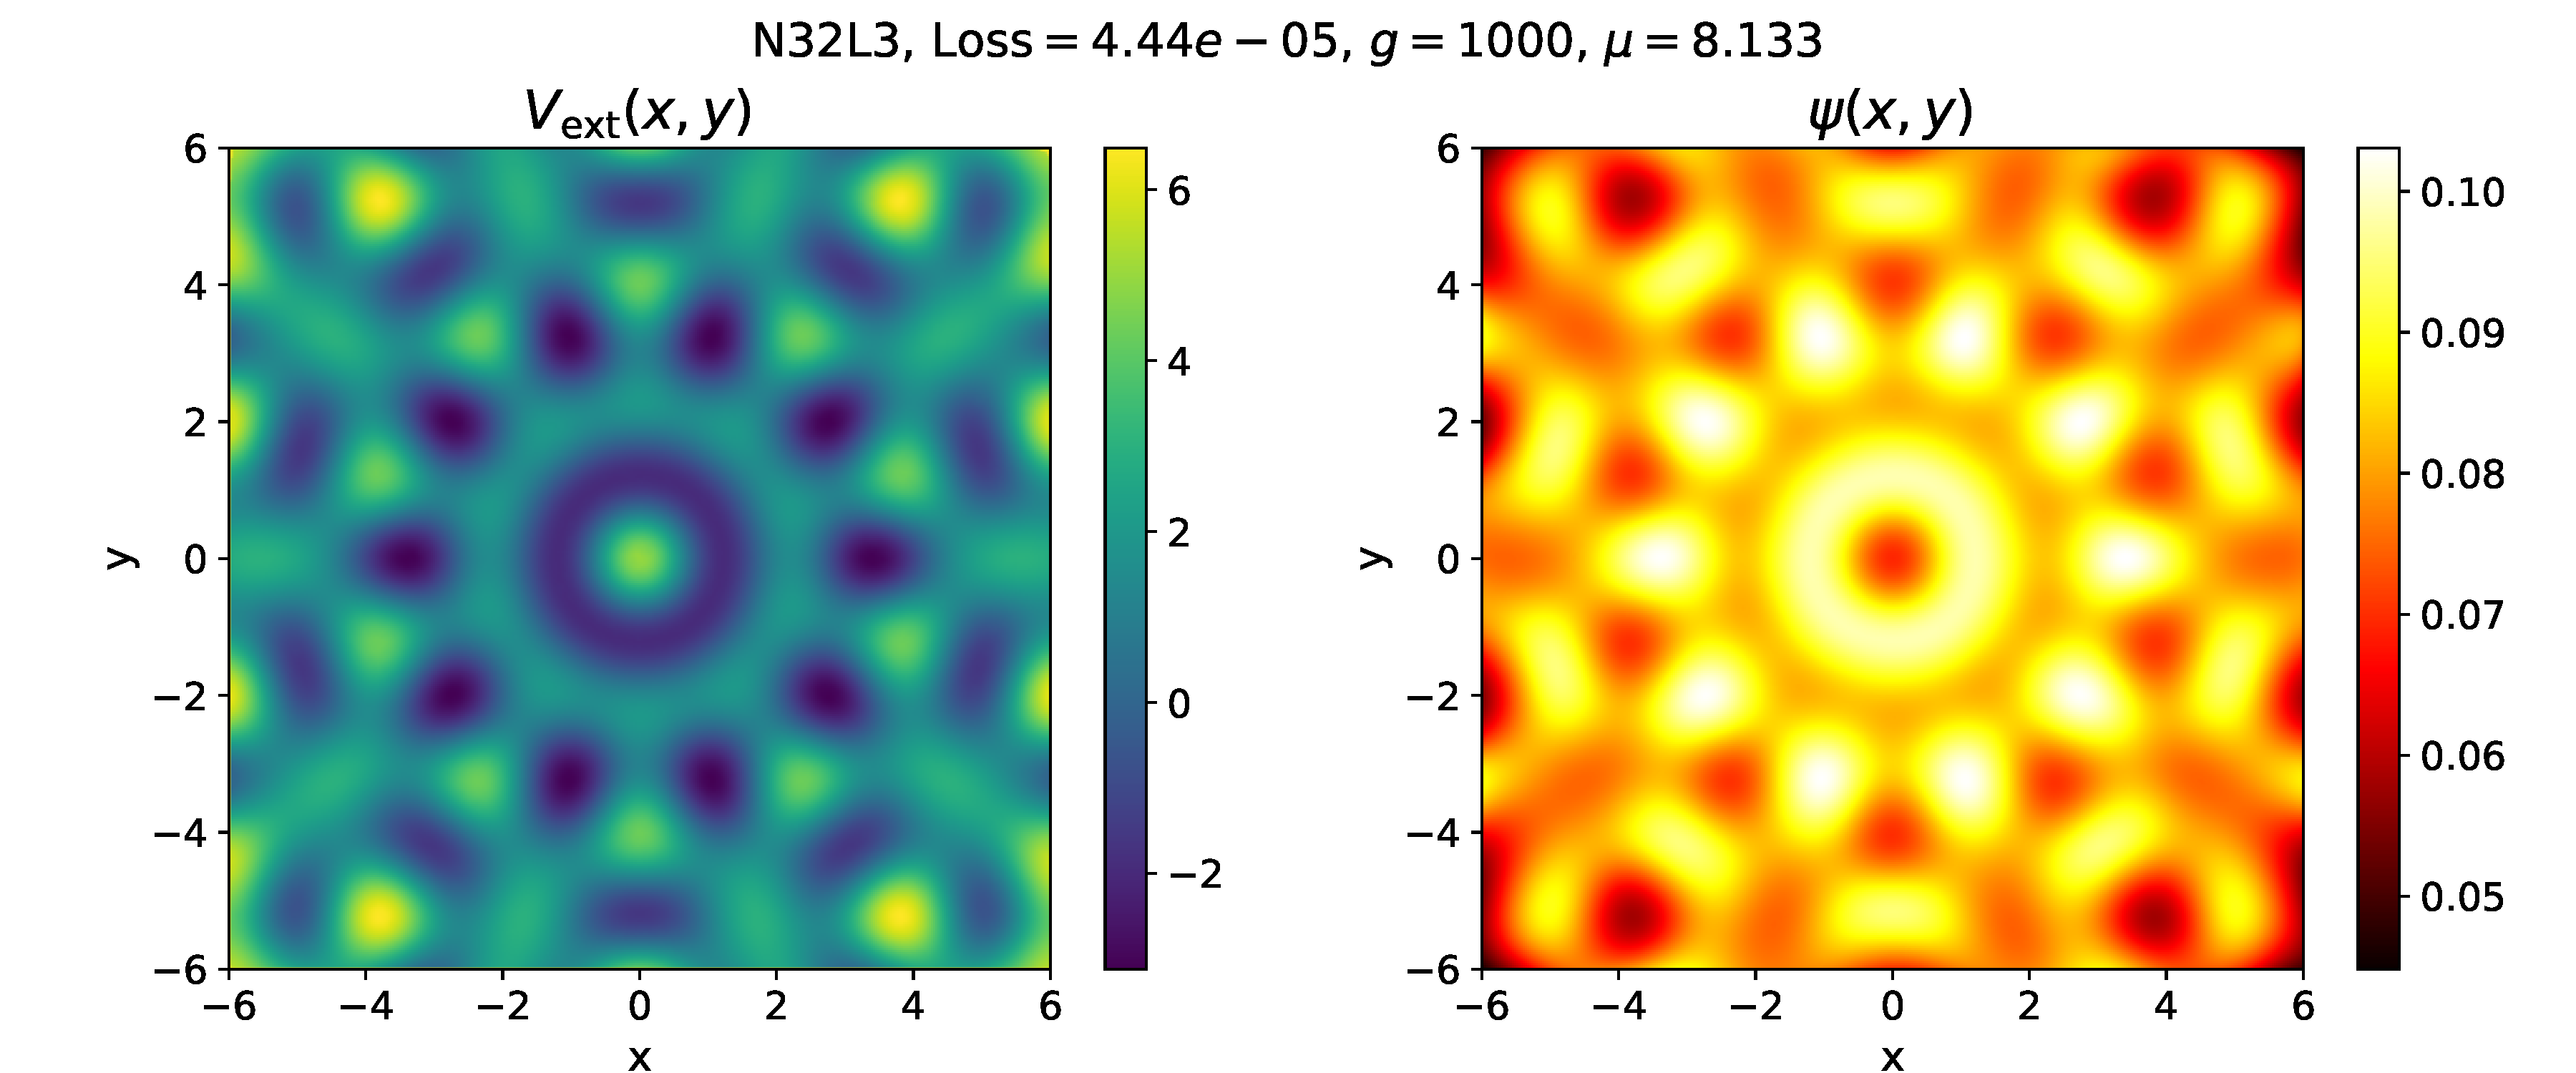
\includegraphics[width=\textwidth]{Figures/ex3_2D_N32L3_g1000_quasicrystal_V01.0_d2.0_omega0.1.png}
    \caption{External potential $V_{\rm ext}(x,y)$ defined in
    \eqref{eq:spread_out_potential} (left) and corresponding ground-state
    solution $\psi(x,y)$ (right) obtained with an N32L3 network for
    $g=1000$. The strong interaction leads to a wave function that spreads
    over multiple rings of local minima.}
    \label{fig:ex3_quasicrystal_g1000}
\end{figure}

\begin{figure}[h]
    \centering
    \begin{minipage}{0.48\textwidth}
        \centering
        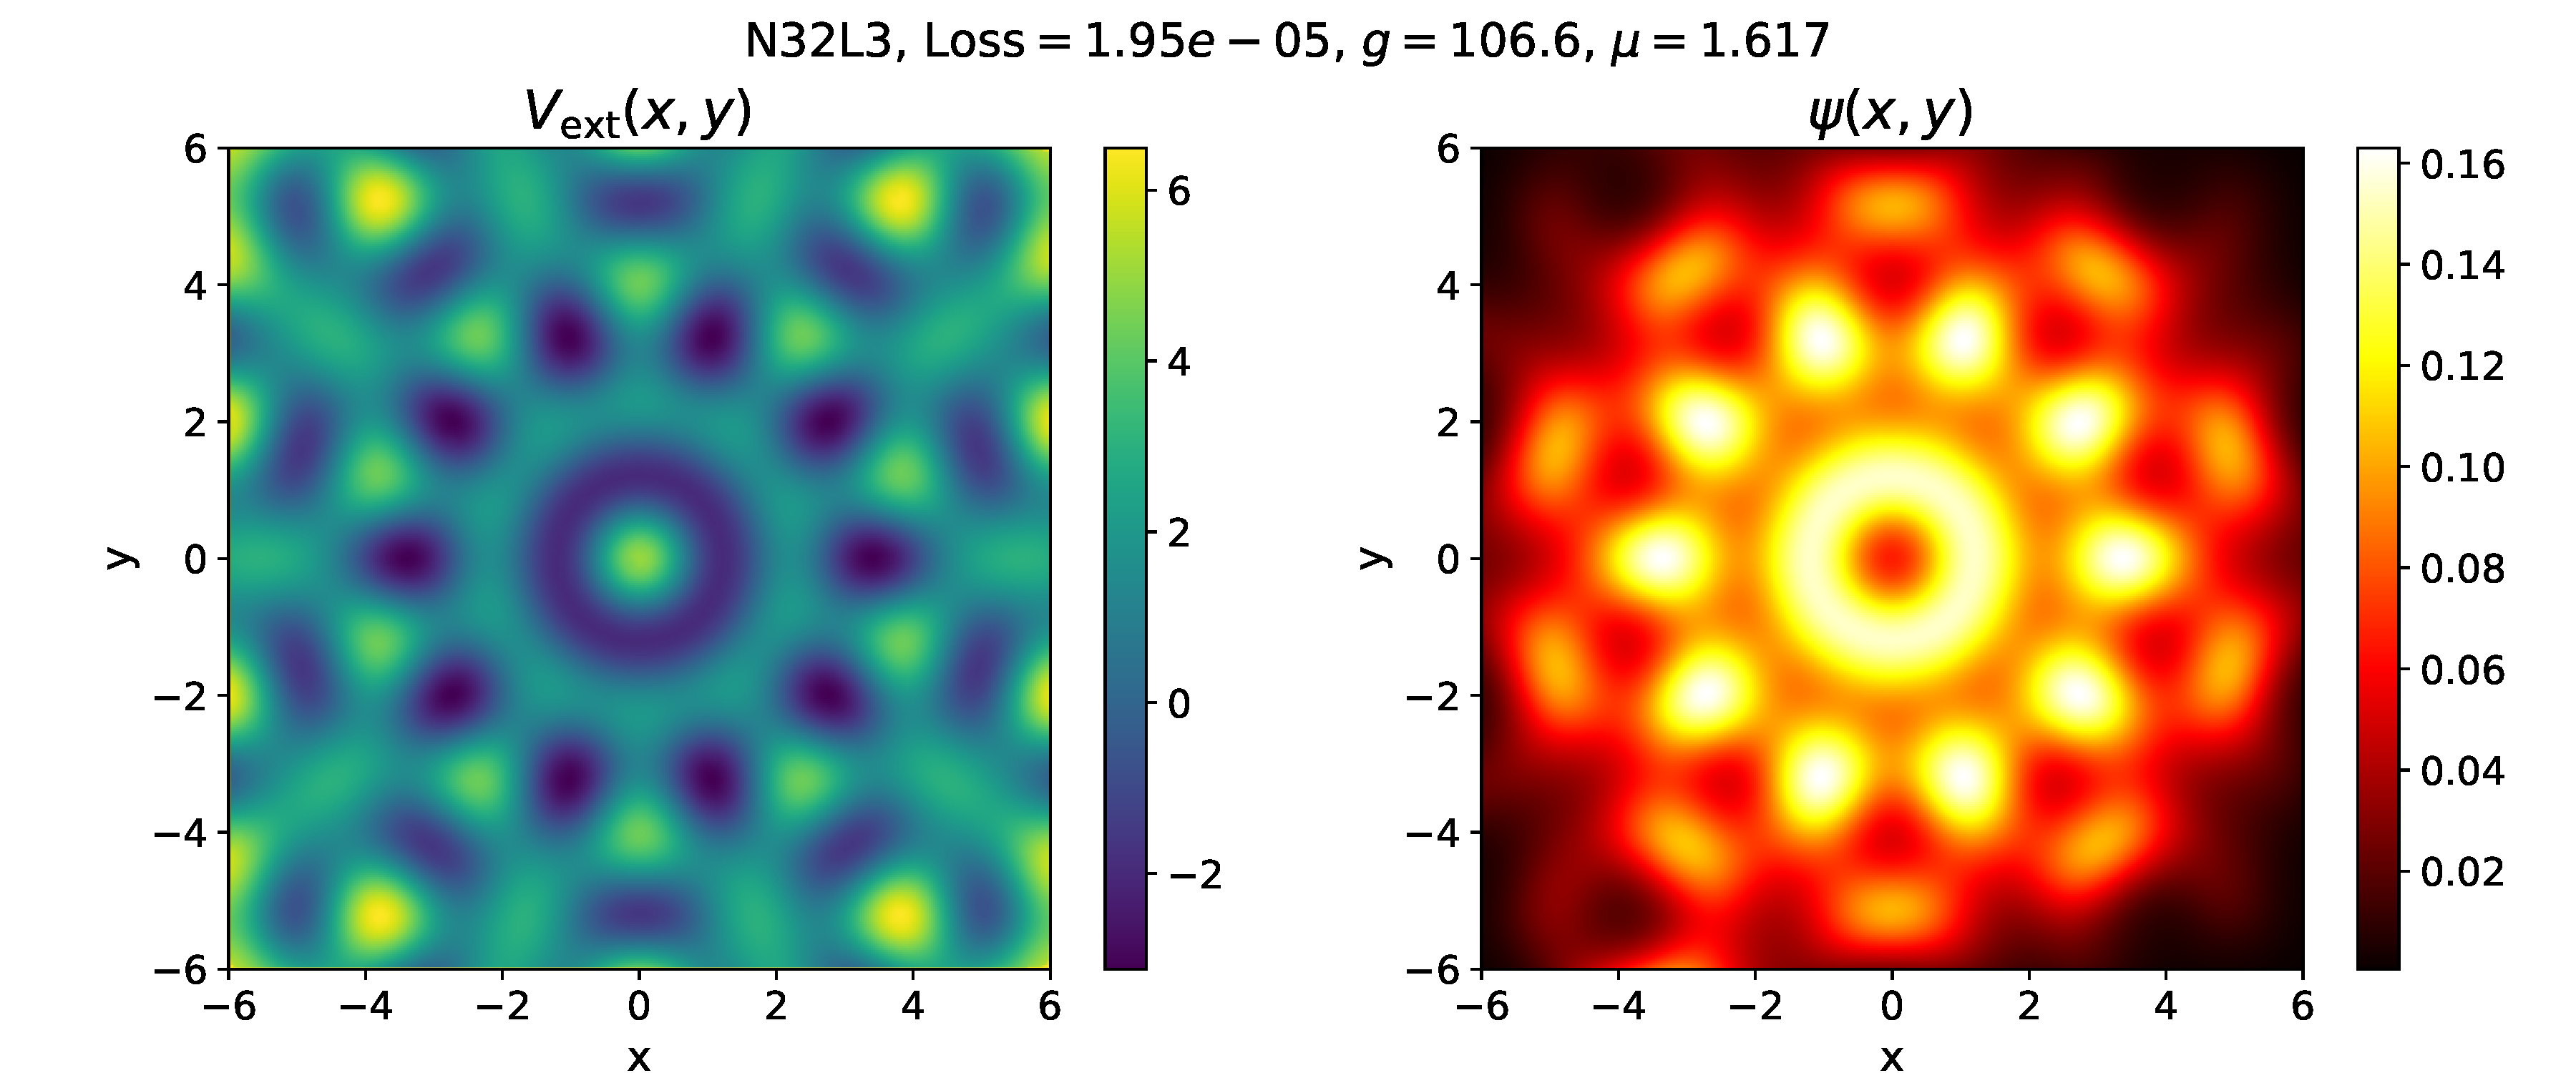
\includegraphics[trim=450 0 0 25, clip, width=\textwidth]
        {Figures/ex3_2D_N32L3_g106.6_quasicrystal_V01.0_d2.0_omega0.1.png}
    \end{minipage}
    \begin{minipage}{0.48\textwidth}
        \centering
        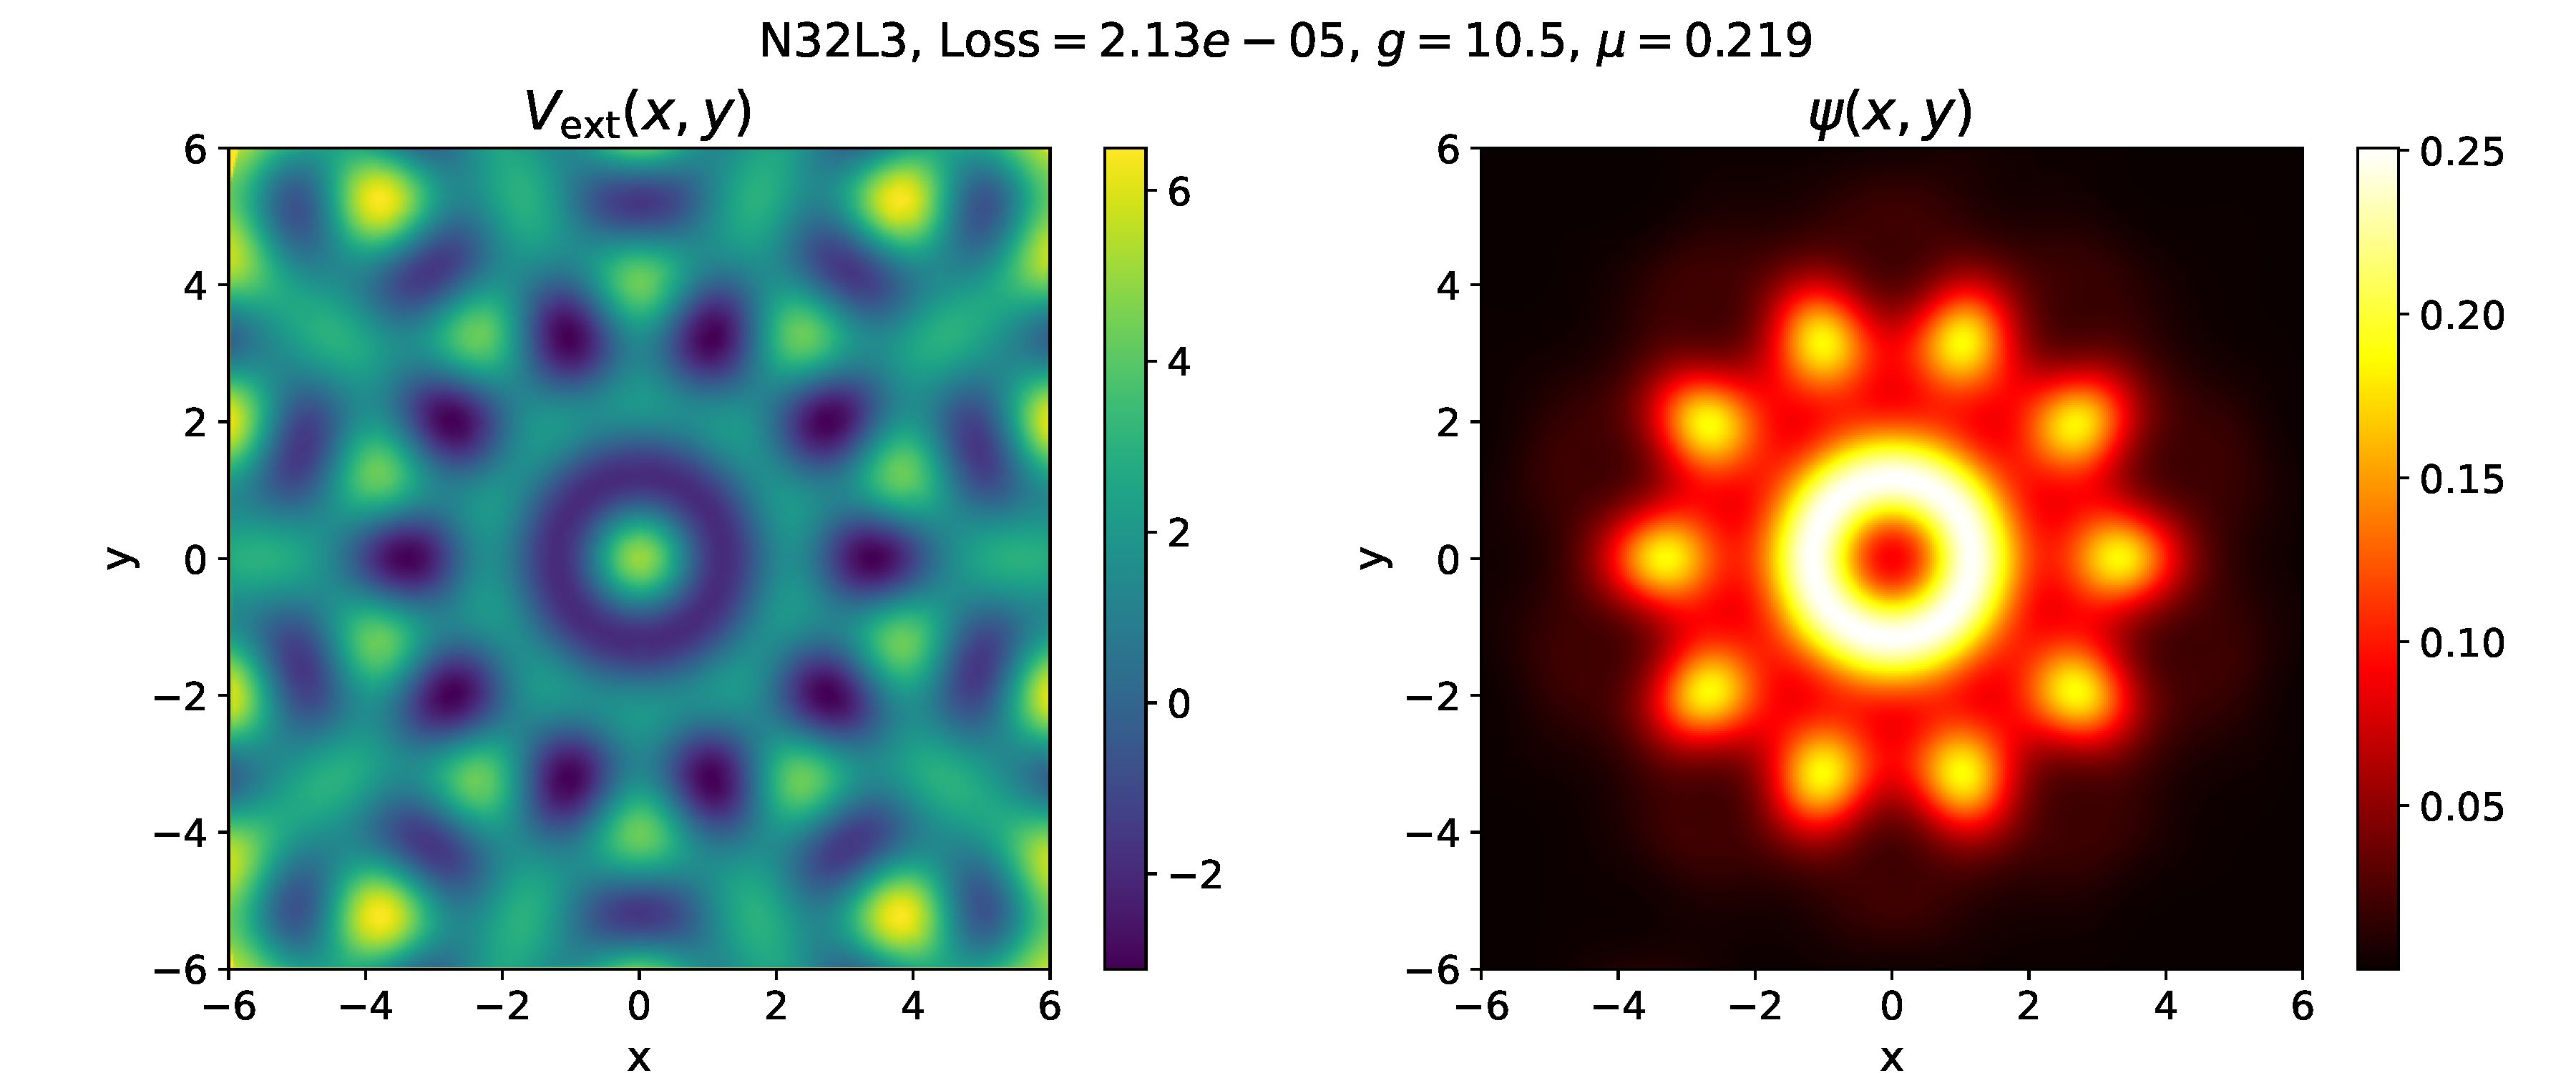
\includegraphics[trim=450 0 0 25, clip, width=\textwidth]
        {Figures/ex3_2D_N32L3_g10.5_quasicrystal_V01.0_d2.0_omega0.1.png}
    \end{minipage}
    \caption{Ground-state solutions $\psi(x,y)$ obtained during the
    continuation procedure as $g$ is reduced.
    Left: $g=106.6$. Right: $g=10.5$.
    As the interaction strength decreases, the solution becomes progressively
    more localized around the energetically favorable rings.}
    \label{fig:ex3_quasicrystal_intermediate}
\end{figure}

\begin{figure}[ht]
    \centering
    \begin{minipage}{0.48\textwidth}
        \centering
        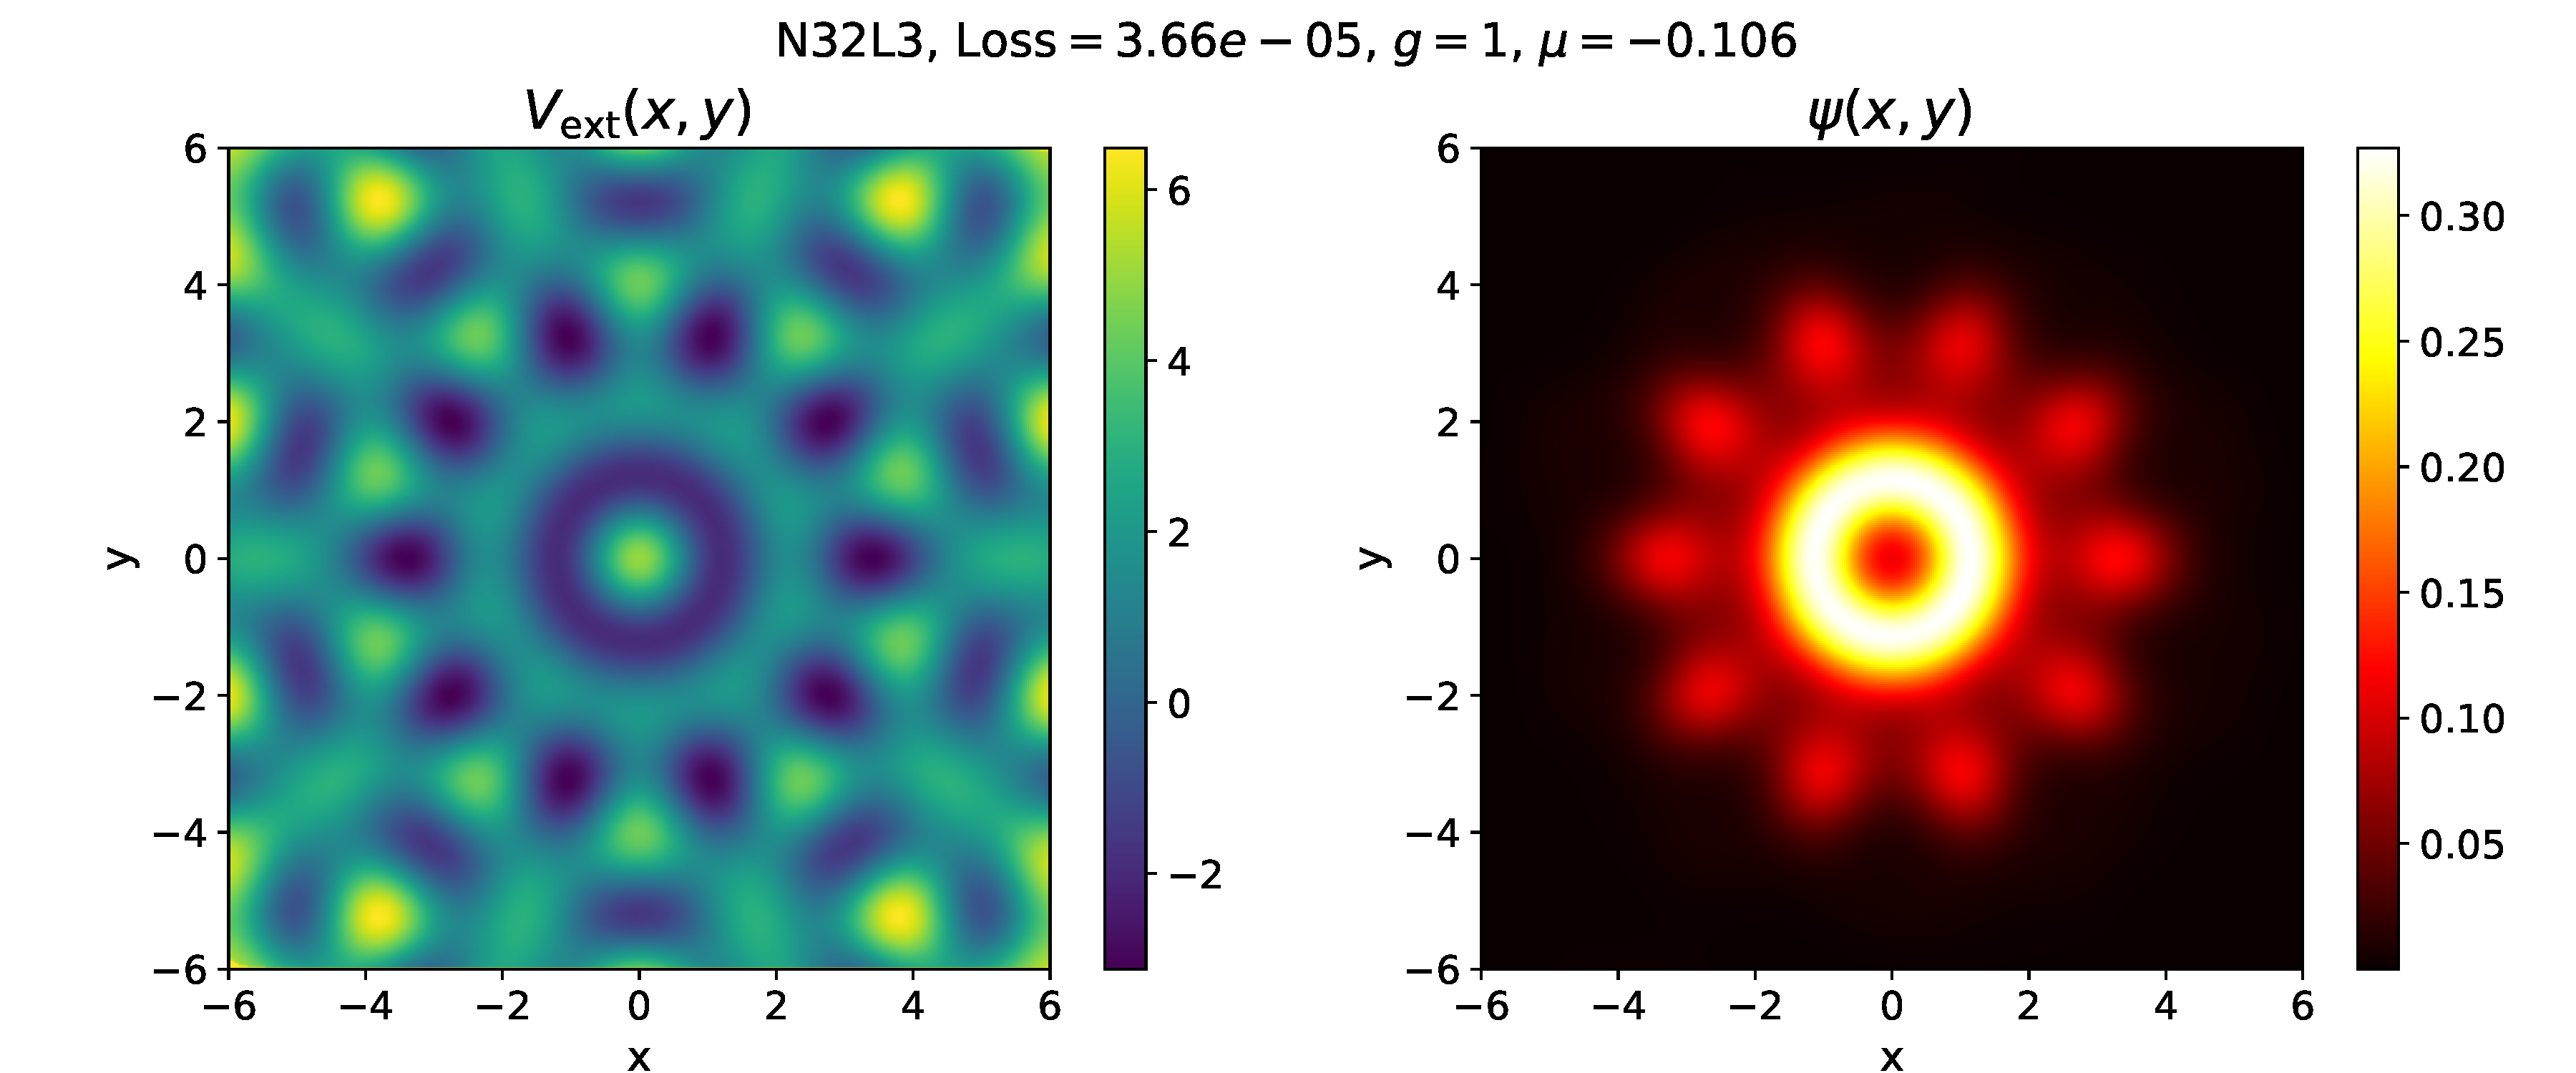
\includegraphics[trim=450 0 0 25, clip, width=\textwidth]
        {Figures/ex3_2D_N32L3_g1_quasicrystal_V01.0_d2.0_omega0.1_more_points.png}
    \end{minipage}
    \begin{minipage}{0.48\textwidth}
        \centering
        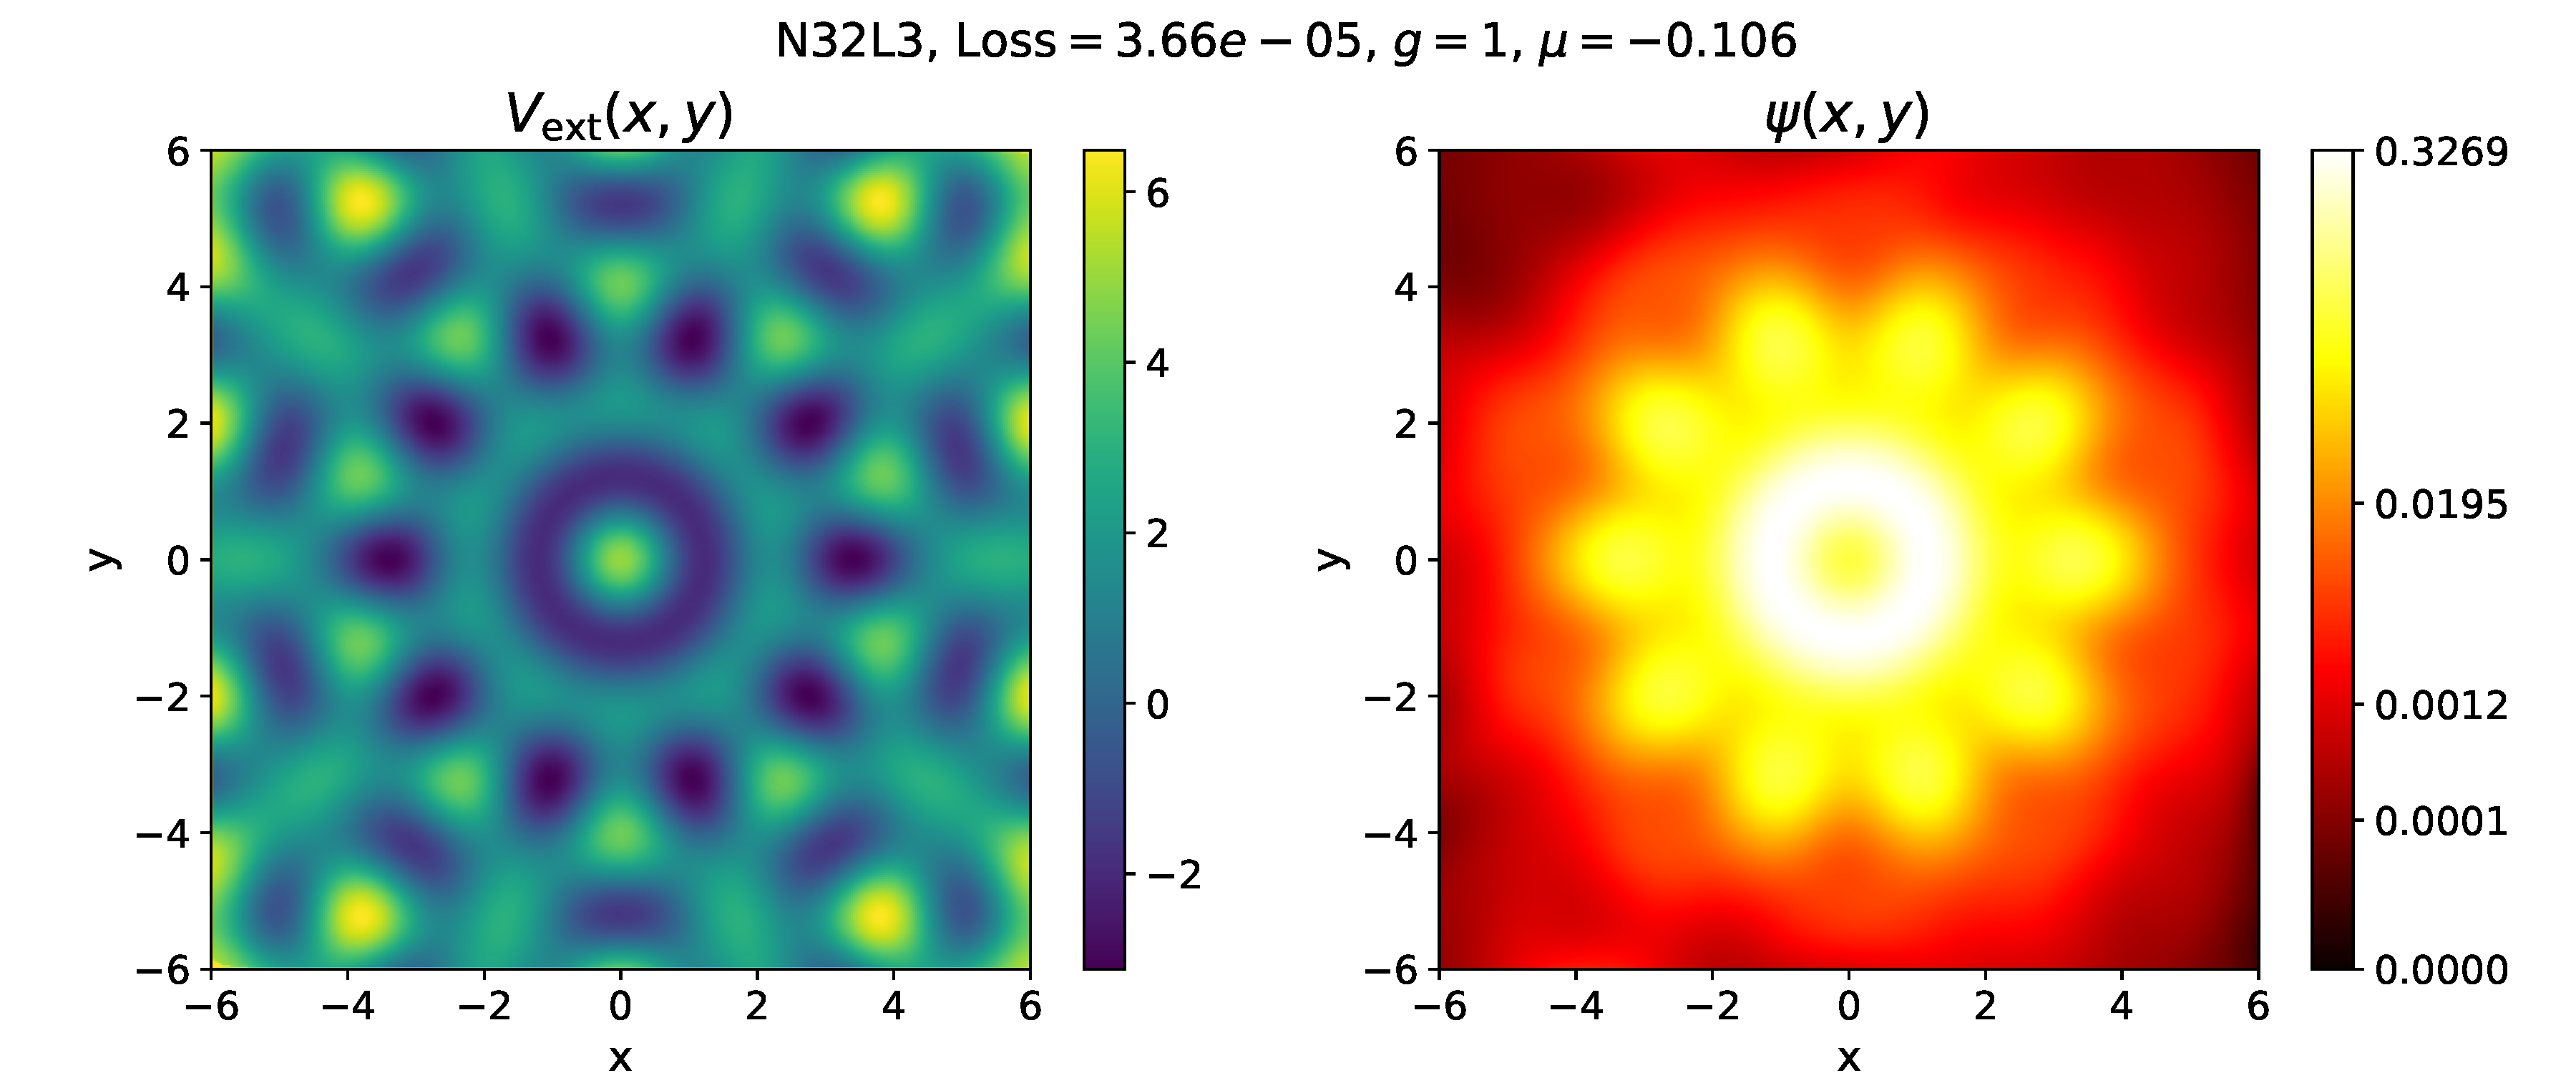
\includegraphics[trim=450 0 0 25, clip, width=\textwidth]
        {Figures/ex3_2D_N32L3_g1_quasicrystal_V01.0_d2.0_omega0.1_more_points_zoom.png}
    \end{minipage}
    \caption{Ground-state solution for $g=1$ computed with additional
    sampling points to improve resolution.
    On the right we stretch the color scale to better visualize the value of the
    wave function close to 0 and observe that the solution still conserves the
    shape of the potential in the outer ring of wells.
    For weak interactions, the wave function concentrates primarily in the
    innermost ring, even though the middle wells are deeper.}
    \label{fig:ex3_quasicrystal_g1}
\end{figure}


\newpage
\printbibliography
\end{document}
